% Options for packages loaded elsewhere
\PassOptionsToPackage{unicode}{hyperref}
\PassOptionsToPackage{hyphens}{url}
\PassOptionsToPackage{dvipsnames,svgnames,x11names}{xcolor}
%
\documentclass[
  10pt,
]{article}
\usepackage{amsmath,amssymb}
\usepackage{iftex}
\ifPDFTeX
  \usepackage[T1]{fontenc}
  \usepackage[utf8]{inputenc}
  \usepackage{textcomp} % provide euro and other symbols
\else % if luatex or xetex
  \usepackage{unicode-math} % this also loads fontspec
  \defaultfontfeatures{Scale=MatchLowercase}
  \defaultfontfeatures[\rmfamily]{Ligatures=TeX,Scale=1}
\fi
\usepackage{lmodern}
\ifPDFTeX\else
  % xetex/luatex font selection
  \setmainfont[]{DejaVu Serif}
  \setsansfont[]{DejaVu Sans}
  \setmonofont[]{DejaVu Sans Mono}
  \setmathfont[]{Latin Modern Math}
\fi
% Use upquote if available, for straight quotes in verbatim environments
\IfFileExists{upquote.sty}{\usepackage{upquote}}{}
\IfFileExists{microtype.sty}{% use microtype if available
  \usepackage[]{microtype}
  \UseMicrotypeSet[protrusion]{basicmath} % disable protrusion for tt fonts
}{}
\makeatletter
\@ifundefined{KOMAClassName}{% if non-KOMA class
  \IfFileExists{parskip.sty}{%
    \usepackage{parskip}
  }{% else
    \setlength{\parindent}{0pt}
    \setlength{\parskip}{6pt plus 2pt minus 1pt}}
}{% if KOMA class
  \KOMAoptions{parskip=half}}
\makeatother
\usepackage{xcolor}
\usepackage[margin=2.0cm]{geometry}
\usepackage{color}
\usepackage{fancyvrb}
\newcommand{\VerbBar}{|}
\newcommand{\VERB}{\Verb[commandchars=\\\{\}]}
\DefineVerbatimEnvironment{Highlighting}{Verbatim}{commandchars=\\\{\}}
% Add ',fontsize=\small' for more characters per line
\newenvironment{Shaded}{}{}
\newcommand{\AlertTok}[1]{\textcolor[rgb]{1.00,0.00,0.00}{\textbf{#1}}}
\newcommand{\AnnotationTok}[1]{\textcolor[rgb]{0.38,0.63,0.69}{\textbf{\textit{#1}}}}
\newcommand{\AttributeTok}[1]{\textcolor[rgb]{0.49,0.56,0.16}{#1}}
\newcommand{\BaseNTok}[1]{\textcolor[rgb]{0.25,0.63,0.44}{#1}}
\newcommand{\BuiltInTok}[1]{\textcolor[rgb]{0.00,0.50,0.00}{#1}}
\newcommand{\CharTok}[1]{\textcolor[rgb]{0.25,0.44,0.63}{#1}}
\newcommand{\CommentTok}[1]{\textcolor[rgb]{0.38,0.63,0.69}{\textit{#1}}}
\newcommand{\CommentVarTok}[1]{\textcolor[rgb]{0.38,0.63,0.69}{\textbf{\textit{#1}}}}
\newcommand{\ConstantTok}[1]{\textcolor[rgb]{0.53,0.00,0.00}{#1}}
\newcommand{\ControlFlowTok}[1]{\textcolor[rgb]{0.00,0.44,0.13}{\textbf{#1}}}
\newcommand{\DataTypeTok}[1]{\textcolor[rgb]{0.56,0.13,0.00}{#1}}
\newcommand{\DecValTok}[1]{\textcolor[rgb]{0.25,0.63,0.44}{#1}}
\newcommand{\DocumentationTok}[1]{\textcolor[rgb]{0.73,0.13,0.13}{\textit{#1}}}
\newcommand{\ErrorTok}[1]{\textcolor[rgb]{1.00,0.00,0.00}{\textbf{#1}}}
\newcommand{\ExtensionTok}[1]{#1}
\newcommand{\FloatTok}[1]{\textcolor[rgb]{0.25,0.63,0.44}{#1}}
\newcommand{\FunctionTok}[1]{\textcolor[rgb]{0.02,0.16,0.49}{#1}}
\newcommand{\ImportTok}[1]{\textcolor[rgb]{0.00,0.50,0.00}{\textbf{#1}}}
\newcommand{\InformationTok}[1]{\textcolor[rgb]{0.38,0.63,0.69}{\textbf{\textit{#1}}}}
\newcommand{\KeywordTok}[1]{\textcolor[rgb]{0.00,0.44,0.13}{\textbf{#1}}}
\newcommand{\NormalTok}[1]{#1}
\newcommand{\OperatorTok}[1]{\textcolor[rgb]{0.40,0.40,0.40}{#1}}
\newcommand{\OtherTok}[1]{\textcolor[rgb]{0.00,0.44,0.13}{#1}}
\newcommand{\PreprocessorTok}[1]{\textcolor[rgb]{0.74,0.48,0.00}{#1}}
\newcommand{\RegionMarkerTok}[1]{#1}
\newcommand{\SpecialCharTok}[1]{\textcolor[rgb]{0.25,0.44,0.63}{#1}}
\newcommand{\SpecialStringTok}[1]{\textcolor[rgb]{0.73,0.40,0.53}{#1}}
\newcommand{\StringTok}[1]{\textcolor[rgb]{0.25,0.44,0.63}{#1}}
\newcommand{\VariableTok}[1]{\textcolor[rgb]{0.10,0.09,0.49}{#1}}
\newcommand{\VerbatimStringTok}[1]{\textcolor[rgb]{0.25,0.44,0.63}{#1}}
\newcommand{\WarningTok}[1]{\textcolor[rgb]{0.38,0.63,0.69}{\textbf{\textit{#1}}}}
\usepackage{longtable,booktabs,array}
\usepackage{calc} % for calculating minipage widths
% Correct order of tables after \paragraph or \subparagraph
\usepackage{etoolbox}
\makeatletter
\patchcmd\longtable{\par}{\if@noskipsec\mbox{}\fi\par}{}{}
\makeatother
% Allow footnotes in longtable head/foot
\IfFileExists{footnotehyper.sty}{\usepackage{footnotehyper}}{\usepackage{footnote}}
\makesavenoteenv{longtable}
\usepackage{graphicx}
\makeatletter
\def\maxwidth{\ifdim\Gin@nat@width>\linewidth\linewidth\else\Gin@nat@width\fi}
\def\maxheight{\ifdim\Gin@nat@height>\textheight\textheight\else\Gin@nat@height\fi}
\makeatother
% Scale images if necessary, so that they will not overflow the page
% margins by default, and it is still possible to overwrite the defaults
% using explicit options in \includegraphics[width, height, ...]{}
\setkeys{Gin}{width=\maxwidth,height=\maxheight,keepaspectratio}
% Set default figure placement to htbp
\makeatletter
\def\fps@figure{htbp}
\makeatother
\setlength{\emergencystretch}{3em} % prevent overfull lines
\providecommand{\tightlist}{%
  \setlength{\itemsep}{0pt}\setlength{\parskip}{0pt}}
\setcounter{secnumdepth}{-\maxdimen} % remove section numbering
% doc_header.tex -- LaTeX preamble additions used by build_docs.sh for every
% Markdown -> LaTeX -> PDF conversion (supplements, README, submission files).
\usepackage{etoolbox}
% longtable may not be loaded by pandoc when a document has no table
\usepackage{longtable}
% bold vectors: \bm -> \symbf under unicode-math (XeLaTeX), bm package otherwise
\makeatletter
\@ifpackageloaded{unicode-math}{\providecommand{\bm}[1]{\symbf{#1}}}{\usepackage{bm}}
\makeatother
% smaller type in long tables so that wide audit tables fit the text width;
% inside a table a line break is allowed after an underscore of plain text
% (pandoc writes it as \_), so that long identifiers wrap inside their column
% rows are set a little apart, so that symbols with indices do not touch
\AtBeginEnvironment{longtable}{\footnotesize\renewcommand{\arraystretch}{1.45}%
  \let\sptunderscore\_\def\_{\sptunderscore\allowbreak}}
\setlength{\LTcapwidth}{\textwidth}
% allow line breaks after slashes and hyphens inside table cells
\usepackage{xurl}
% code blocks: break over-long lines instead of running into the margin.
% Plain ``` blocks are typeset by pandoc as {verbatim}, highlighted ones
% (```bash) as {Highlighting}; both are re-declared as breakable fancyvrb
% environments.  The continuation line is marked with a small hooked arrow.
\usepackage{fvextra}
\RecustomVerbatimEnvironment{verbatim}{Verbatim}{breaklines,breakanywhere,fontsize=\small}
\makeatletter
\@ifundefined{Highlighting}{}{%
  \RecustomVerbatimEnvironment{Highlighting}{Verbatim}{breaklines,breakanywhere,fontsize=\small,commandchars=\\\{\}}}
\makeatother
% inline code (pandoc writes it as \texttt{...}): never hyphenate -- an inserted
% hyphen could be read as part of a file name -- but allow a line break after
% an underscore, slash, comma, colon or equals sign, so that long paths and
% column lists wrap inside the text width and inside table columns.
% Inside a formula (e.g. the name of a notebook symbol in an equation) the same
% command must first leave math mode, which \text of amsmath does.
\ExplSyntaxOn
\tl_new:N \l__spt_code_tl
\cs_new_protected:Npn \__spt_texttt:n #1
  {
    \tl_set:Nn \l__spt_code_tl {#1}
    \regex_replace_all:nnN { ([\/\,\:\=]) } { \1 \c{allowbreak} } \l__spt_code_tl
    \regex_replace_all:nnN { \c{_} } { \c{_} \c{allowbreak} } \l__spt_code_tl
    \group_begin: \ttfamily \hyphenchar \font = -1 \scan_stop: \l__spt_code_tl \group_end:
  }
\RenewDocumentCommand \texttt { m }
  {
    \mode_if_math:TF { \text { \__spt_texttt:n {#1} } } { \__spt_texttt:n {#1} }
  }
\ExplSyntaxOff
% A figure is written in the Markdown source as an image paragraph followed by
% a caption paragraph ("**Figure S1.** ..."), so that the caption is also
% visible on GitHub.  An image that starts a paragraph is centered.
\usepackage{graphicx}% pandoc loads it only for documents that contain an image
\NewCommandCopy\sptincludegraphics\includegraphics
\RenewDocumentCommand\includegraphics{O{} m}{%
  \ifvmode\begin{center}\sptincludegraphics[#1]{#2}\end{center}%
  \else\sptincludegraphics[#1]{#2}\fi}
% keep figures where they are referenced
\usepackage{float}
\floatplacement{figure}{H}
% running header with the document title
\usepackage{fancyhdr}
\pagestyle{fancy}
\fancyhf{}
\fancyhead[L]{\small PROJECT spacetimes, Revision\_Deflation --- documentation and provenance}
\fancyhead[R]{\small\thepage}
\renewcommand{\headrulewidth}{0.4pt}
% 16x16 matrices: tighter columns so that a full matrix fits the text width
\setlength{\arraycolsep}{3.2pt}
% The documents of this project contain long tagged symbols, file paths and
% identifiers that cannot be hyphenated.  A paragraph is therefore allowed to
% have looser lines before TeX gives up and lets a line stick out of the margin.
\AtBeginDocument{\tolerance=2000 \emergencystretch=5em \hbadness=2000}
\ifLuaTeX
  \usepackage{selnolig}  % disable illegal ligatures
\fi
\IfFileExists{bookmark.sty}{\usepackage{bookmark}}{\usepackage{hyperref}}
\IfFileExists{xurl.sty}{\usepackage{xurl}}{} % add URL line breaks if available
\urlstyle{same}
\hypersetup{
  pdftitle={dirac matrices deflating --- geometry, Dirac matrices, spin connection, Dirac equations and their solutions on the 4+4 and 7+1 spacetimes whose coordinates x5, x6, x7 deflate exponentially},
  pdfauthor={Prepared for Patrick Lee Nash, Ph.D.},
  colorlinks=true,
  linkcolor={blue},
  filecolor={Maroon},
  citecolor={blue},
  urlcolor={blue},
  pdfcreator={LaTeX via pandoc}}

\title{dirac matrices deflating --- geometry, Dirac matrices, spin
connection, Dirac equations and their solutions on the 4+4 and 7+1
spacetimes whose coordinates x5, x6, x7 deflate exponentially}
\usepackage{etoolbox}
\makeatletter
\providecommand{\subtitle}[1]{% add subtitle to \maketitle
  \apptocmd{\@title}{\par {\large #1 \par}}{}{}
}
\makeatother
\subtitle{PROJECT spacetimes, Revision\_Deflation. Provenance:
definitions, derivations, machine checks, and how to reproduce them}
\author{Prepared for Patrick Lee Nash, Ph.D.}
\date{November 12, 2026}

\begin{document}
\maketitle

\hypertarget{what-this-document-proves-and-for-whom}{%
\section{0. What this document proves, and for
whom}\label{what-this-document-proves-and-for-whom}}

The main project studies a 16-component Dirac field on two flat
eight-dimensional spacetimes: one of signature \textbf{4+4} (four
space-like and four time-like coordinates) and one of signature
\textbf{7+1} (seven space-like coordinates and one time-like
coordinate). Its document \texttt{dirac\ matrices} (in the folder above
this one) displays the eight real 16×16 Dirac matrices of each
spacetime, proves their properties and writes down the Dirac equations
of the fields \textbf{dirac1644} and \textbf{dirac1671}.

The revision replaces the two flat spacetimes by two curved ones, in
which three of the eight coordinates shrink as the ordinary time
advances. This document repeats, for the curved spacetimes, everything
that \texttt{dirac\ matrices} does for the flat ones. It is written for
a reader who has worked through \texttt{dirac\ matrices} and who knows
general relativity at the level of a first course: metric, Christoffel
symbols, curvature, geodesics. What such a course usually omits --- how
a spinor is differentiated on a curved spacetime --- is derived here
from the beginning (Part 2).

\begin{itemize}
\tightlist
\item
  \textbf{Part 1} is geometry: the metric, its Christoffel symbols, its
  curvature, its Einstein tensor, its symmetries and its geodesics.
\item
  \textbf{Part 2} constructs the Dirac matrices of the curved spacetimes
  and the spin connection, which is the object that tells a spinor how
  to follow the curvature.
\item
  \textbf{Part 3} writes down the Dirac equations of the two fields of
  the revision, \textbf{dirac1644d} and \textbf{dirac1671d}, and brings
  them to the form in which they are solved.
\item
  \textbf{Part 4} solves them, mode by mode, in closed form where that
  is possible and numerically where it is not. Two results stand out. On
  the 7+1 spacetime the deflation \emph{creates particles}, with a
  thermal spectrum whose temperature is the rate of deflation divided by
  \(2\pi\). On the 4+4 spacetime the deflation \emph{extinguishes} every
  dependence of the field on the three deflating times.
\item
  \textbf{Part 5} states which symmetries of the flat spacetimes
  survive.
\item
  \textbf{Part 6} separates what has been established from what has not.
\end{itemize}

\textbf{How the statements are verified.} Each statement of Parts 1 to 3
is an identity between rational functions of the rates and of the scale
factors. The Rust program \texttt{deflation} (folder
\texttt{code/deflation-rs}) verifies each identity in exact rational
arithmetic at five sets of rational values of the parameters; each
verification has an identifier such as \texttt{44d-C4} (the prefix
\texttt{44d-} refers to the deflating 4+4 spacetime, \texttt{71d-} to
the deflating 7+1 spacetime, \texttt{def-} to both). An independent
Python script verifies the same identities \emph{symbolically}, for
arbitrary values of the parameters, by computer algebra; its identifiers
begin with the letter \texttt{I}. The statements of Part 4 are verified
numerically by two different integration methods in two languages. The
complete output of all programs is reproduced verbatim in Appendix A.

\hypertarget{the-hypotheses}{%
\subsection{0.1 The hypotheses}\label{the-hypotheses}}

The hypotheses are the author's. In his words, the coordinates \(x5\),
\(x6\) and \(x7\) \emph{deflate exponentially}, on the 4+4 spacetime and
on the 7+1 spacetime alike, and Minkowski space is replaced by a
pseudo-Riemannian space with a diagonal metric. For the 4+4 spacetime he
specified the three components of the metric that change:
\[g_{55}=-\,\mathrm{const5}^2\,e^{-2\,\mathrm{g55}\,x4},\qquad
g_{66}=-\,\mathrm{const6}^2\,e^{-2\,\mathrm{g66}\,x4},\qquad
g_{77}=-\,\mathrm{const7}^2\,e^{-2\,\mathrm{g77}\,x4},\tag{0.1}\] with
three positive rates \(\mathrm{g55}\), \(\mathrm{g66}\),
\(\mathrm{g77}\) and three positive constants, which may differ from one
another. (The author writes one word, const, for the three constants;
because they may differ they are given three names here.) The other five
components of the metric keep their flat values.

\emph{The names.} \(\mathrm{g55}\), \(\mathrm{g66}\) and
\(\mathrm{g77}\) are the author's names for the three \textbf{rates}.
They are written upright and without a subscript throughout the
revision. The three \textbf{components of the metric} are written with
subscripts, \(g_{55}\), \(g_{66}\), \(g_{77}\). Equation (0.1) shows the
two side by side: the rate \(\mathrm{g55}\) is the number in the
exponent of the component \(g_{55}\) of the metric.

\emph{The 7+1 spacetime.} For the 7+1 spacetime the author wrote the
same three exponentials with a positive sign, which is their form in a
convention that gives space-like components of the metric the positive
sign. The main project writes the 7+1 metric with the opposite
convention, \(\eta_{1671}=\mathrm{diag}(-1,-1,-1,-1,+1,-1,-1,-1)\), in
which the time-like component is positive. In that convention the three
components of the metric are again those of Eq. (0.1), with the minus
signs. The geometry is the same in either convention: the proper length
of a coordinate interval along \(x5\) is
\(\mathrm{const5}\,e^{-\mathrm{g55}\,x4}\) times the coordinate
interval. Equation (0.1) therefore holds on both spacetimes in the
conventions of this project; what differs is the meaning of the sign. On
the 7+1 spacetime \(x5\), \(x6\), \(x7\) are three of the seven
space-like coordinates, and what deflates is a \emph{length}. On the 4+4
spacetime they are three of the four time-like coordinates, and what
deflates is a \emph{duration} measured along an additional time.

\emph{What ``deflates'' means.} The coordinate \(x4\) is the ordinary
time. As \(x4\) increases by \(1/\mathrm{g55}\), every proper interval
along \(x5\) shrinks by the factor \(e\). The word is the opposite of
inflation, in which lengths grow exponentially.

\emph{Tags.} The flat spacetimes and their objects carry the tags 1644
and 1671 in the main project. The deflating spacetimes and their objects
carry the tags \textbf{1644d} and \textbf{1671d}. A general coordinate
among the three deflating ones is written \(xt\) with \(t\in\{5,6,7\}\),
and its rate is written \(\mathrm{rate}_t\), so that
\(\mathrm{rate}_5=\mathrm{g55}\), \(\mathrm{rate}_6=\mathrm{g66}\),
\(\mathrm{rate}_7=\mathrm{g77}\). A general coordinate among
\(x0,x1,x2,x3\) is written \(xa\).

\hypertarget{the-unique-symbols-of-this-document}{%
\subsection{0.2 The unique symbols of this
document}\label{the-unique-symbols-of-this-document}}

The main project keeps a MASTER registry of symbols in which every
symbol has one meaning. The revision adds the symbols below to it; the
provenance RP1 proves by machine that none of them collides with a
symbol of the main registry or with a symbol of the author's notebooks.
The column ``in programs and data files'' gives the spelling of the same
object in the Rust program and in the data files.

\begin{longtable}[]{@{}
  >{\raggedright\arraybackslash}p{(\columnwidth - 8\tabcolsep) * \real{0.1379}}
  >{\raggedright\arraybackslash}p{(\columnwidth - 8\tabcolsep) * \real{0.1379}}
  >{\raggedright\arraybackslash}p{(\columnwidth - 8\tabcolsep) * \real{0.4483}}
  >{\raggedright\arraybackslash}p{(\columnwidth - 8\tabcolsep) * \real{0.1379}}
  >{\raggedright\arraybackslash}p{(\columnwidth - 8\tabcolsep) * \real{0.1379}}@{}}
\toprule\noalign{}
\begin{minipage}[b]{\linewidth}\raggedright
symbol
\end{minipage} & \begin{minipage}[b]{\linewidth}\raggedright
in programs and data files
\end{minipage} & \begin{minipage}[b]{\linewidth}\raggedright
meaning
\end{minipage} & \begin{minipage}[b]{\linewidth}\raggedright
defined in
\end{minipage} & \begin{minipage}[b]{\linewidth}\raggedright
origin
\end{minipage} \\
\midrule\noalign{}
\endhead
\bottomrule\noalign{}
\endlastfoot
\(\mathrm{g55}\), \(\mathrm{g66}\), \(\mathrm{g77}\) & \texttt{g55},
\texttt{g66}, \texttt{g77} & the three rates of deflation of \(x5\),
\(x6\), \(x7\) (positive constants, dimension 1/length). These are the
author's names; they are written upright and never with a subscript.
They are \emph{not} components of the metric: the components are
\(g_{55}\), \(g_{66}\), \(g_{77}\) & RP0 1; DMD 0.1; M II & author \\
\(\mathrm{rate}_t\) & \texttt{rate\_t}, \texttt{rate} & the rate of the
coordinate \(xt\) in a statement that holds for \(t=5,6,7\) alike:
\(\mathrm{rate}_5=\mathrm{g55}\), \(\mathrm{rate}_6=\mathrm{g66}\),
\(\mathrm{rate}_7=\mathrm{g77}\) & DMD 0.1 & new \\
\(\mathrm{gsum}\) & \texttt{gsum}, \texttt{gam} &
\(\mathrm{g55}+\mathrm{g66}+\mathrm{g77}\), the total rate: the proper
volume of the three deflating coordinates falls as
\(e^{-\mathrm{gsum}\,x4}\) (\texttt{gam}: gsum in units of 100 km/s/Mpc)
& DMD 1.1; M II & new \\
\(\mathrm{gsq}\), \(\mathrm{gprod}\) & \texttt{gsq}, \texttt{gprod} &
\(\mathrm{g55}^2+\mathrm{g66}^2+\mathrm{g77}^2\) and
\(\mathrm{g55}\,\mathrm{g66}+\mathrm{g55}\,\mathrm{g77}+\mathrm{g66}\,\mathrm{g77}\);
\(\mathrm{gsum}^2=\mathrm{gsq}+2\,\mathrm{gprod}\) & DMD 1.3 & new \\
\(\mathrm{const5}\), \(\mathrm{const6}\), \(\mathrm{const7}\);
\(\mathrm{const}_t\) & \texttt{const5}, \texttt{const6},
\texttt{const7}, \texttt{const\_t}, \texttt{cst} & the three positive
constants of the author's metric (his word: const): the values of the
scale factors at \(x4=0\) & RP0 1; DMD 0.1 & author \\
\(b_5\), \(b_6\), \(b_7\); \(b_t\) & \texttt{b\_5}, \texttt{b\_6},
\texttt{b\_7}, \texttt{b\_t} & the scale factors of the deflating
coordinates, \(b_t(x4)=\mathrm{const}_t\,e^{-\mathrm{rate}_t\,x4}\): a
coordinate distance \(dxt\) is the proper length
\(b_t\,\lvert dxt\rvert\). Always written with the index 5, 6, 7 or
\(t\) (the letter \(b\) without index is a Ginzburg-Landau coefficient
of the main registry) & DMD 1.1; M II & new \\
\(V_d\) & \texttt{Vd} & \(b_5b_6b_7=\sqrt{\lvert\det g\rvert}\), the
proper volume of a unit coordinate cell of the deflating coordinates;
\(V_d\propto e^{-\mathrm{gsum}\,x4}\) & DMD 1.1; RS1 1 & new \\
\(g_{1644d}\), \(g_{1671d}\); \(g_{\mu\nu}\) & \texttt{g\_1644d},
\texttt{g\_1671d} & the metrics of the deflating 4+4 and 7+1 spacetimes,
\(\mathrm{diag}(\eta_{00},\dots,\eta_{44},\eta_{55}b_5^2,\eta_{66}b_6^2,\eta_{77}b_7^2)\)
with \(\eta=\eta_{1644}\) or \(\eta_{1671}\); in both,
\(g_{tt}=-\mathrm{const}_t^2e^{-2\,\mathrm{rate}_t\,x4}\) & DMD 1.1 &
author \\
\(\mu,\nu,\rho,\sigma\) (indices) & \texttt{mu}, \texttt{nu},
\texttt{rho}, \texttt{sigma}, \texttt{lam} & coordinate indices with the
values \(0,\dots,7\) on the deflating spacetimes (only as sub- or
superscripts; as stand-alone letters \(\mu\), \(\nu\), \(\lambda\) keep
the meanings of the main registry). The capital indices \(A,B\) label
the orthonormal frame: the frame vector \(A\) points along the
coordinate \(xA\) & DMD 1.1 & new \\
\(e_A{}^\mu\), \(e^A{}_\mu\) & \texttt{e\_A\^{}mu} & the orthonormal
frame and its inverse:
\(e^A{}_\mu=\mathrm{diag}(1,1,1,1,1,b_5,b_6,b_7)\) & DMD 1.1 & new \\
\(\Gamma^\rho{}_{\mu\nu}\) & \texttt{Gamma}, \texttt{christoffel} & the
Christoffel symbols of the deflating metric (three indices; the letter
\(\Gamma\) with square brackets is the effective action of the main
registry) & DMD 1.2 & new \\
\(R^\rho{}_{\sigma\mu\nu}\), \(R^\mu{}_\nu\), \(R\) & \texttt{riemann},
\texttt{ricci}, \texttt{Ric44}, \texttt{Ric55}, \texttt{Ric66},
\texttt{Ric77}, \texttt{Rscalar} & Riemann tensor, Ricci tensor and
curvature scalar of the deflating metric & DMD 1.3 & new \\
\(\mathcal G^\mu{}_\nu\) & \texttt{Ein00}, \texttt{Ein44},
\texttt{Ein55}, \texttt{Ein66}, \texttt{Ein77}, \texttt{einstein\_mixed}
& the Einstein tensor \(R^\mu{}_\nu-\tfrac12R\,\delta^\mu_\nu\) (script
letter, so that it cannot be taken for Newton's constant or for a
constant of the Fermi type) & DMD 1.4 & new \\
\(\mathcal X\); \(\mathcal X_{\rm scale}\), \(\mathcal X_{(s)}\) &
\texttt{killing\_vectors}, \texttt{killing\_count} & a Killing vector
field of the deflating metric (script letter; the plain letter \(X\) is
the set of coordinates of the main registry); the scaling vector
\(\partial_4+\sum_t\mathrm{rate}_t\,xt\,\partial_t\); the three special
Killing vectors of the case of equal rates, \(s=5,6,7\) & DMD 1.5, 1.6 &
new \\
\(\bar x4\); \(\bar x5\), \(\bar x6\), \(\bar x7\) & --- & coordinates
of the case of equal rates in which the line element of \(x4,\dots,x7\)
is a multiple of a flat one:
\(\bar x4=e^{\mathrm{g55}\,x4}/\mathrm{g55}\),
\(\bar xt=\mathrm{const}_t\,xt\) & DMD 1.6 & new \\
\(\varsigma\) & \texttt{affine} & affine parameter along a geodesic; for
a massive particle on the 7+1 spacetime, the proper time divided by the
mass & DMD 1.7 & new \\
\(P_\mu\) & \texttt{P\_1}, \texttt{P\_5} & the conserved covariant
momenta of a geodesic (with an index; \(P\) without index is the
generator of the main registry) & DMD 1.7 & new \\
\(x4_{\rm turn}\) & \texttt{x4\_turn} & the value of the ordinary time
at which a classical particle with momentum along a deflating time turns
back, and beyond which a mode that depends on a deflating time is
extinguished (4+4): there \(k_d=E_\perp\) & DMD 1.7, 4.3 & new \\
\end{longtable}

\begin{longtable}[]{@{}
  >{\raggedright\arraybackslash}p{(\columnwidth - 8\tabcolsep) * \real{0.1379}}
  >{\raggedright\arraybackslash}p{(\columnwidth - 8\tabcolsep) * \real{0.1379}}
  >{\raggedright\arraybackslash}p{(\columnwidth - 8\tabcolsep) * \real{0.4483}}
  >{\raggedright\arraybackslash}p{(\columnwidth - 8\tabcolsep) * \real{0.1379}}
  >{\raggedright\arraybackslash}p{(\columnwidth - 8\tabcolsep) * \real{0.1379}}@{}}
\toprule\noalign{}
\begin{minipage}[b]{\linewidth}\raggedright
symbol
\end{minipage} & \begin{minipage}[b]{\linewidth}\raggedright
in programs and data files
\end{minipage} & \begin{minipage}[b]{\linewidth}\raggedright
meaning
\end{minipage} & \begin{minipage}[b]{\linewidth}\raggedright
defined in
\end{minipage} & \begin{minipage}[b]{\linewidth}\raggedright
origin
\end{minipage} \\
\midrule\noalign{}
\endhead
\bottomrule\noalign{}
\endlastfoot
\(\gamma_{1644d}^\mu\), \(\gamma_{1671d}^\mu\) & \texttt{gamma\_1644d},
\texttt{gamma\_1671d} & the Dirac matrices of the deflating spacetimes
in coordinate components, \(\gamma^\mu=e_A{}^\mu\gamma^A\):
\(\gamma^t=\gamma^{A=t}/b_t\) for \(t=5,6,7\), the other five are the
constant matrices \(\gamma_{1644}^A\), \(\gamma_{1671}^A\) of the main
project & DMD 2.2 & new \\
\(\omega_{\mu AB}\) & \texttt{omega\_(mu}, \texttt{A}, \texttt{B)} & the
coefficients of the spin connection (three indices; \(\omega_{1644}\),
\(\omega_{1671}\) with a tag are the volume elements of the main
registry) & DMD 2.3 & new \\
\(\Omega_\mu\) & \texttt{Omega\_mu}, \texttt{omega} & the spin
connection as a matrix, \(\tfrac14\omega_{\mu AB}\gamma^A\gamma^B\); the
covariant derivative of a spinor is
\(\nabla_\mu\psi=(\partial_\mu+\Omega_\mu)\psi\) & DMD 2.3 & new \\
\(\psi_{1644d}\), \(\psi_{1671d}\) & \texttt{dirac1644d},
\texttt{dirac1671d} & the fields dirac1644d and dirac1671d: the
16-component fields of the main project on the deflating spacetimes;
\((\gamma^\mu\nabla_\mu-m)\psi_{1644d}=0\) and
\((i\gamma^\mu\nabla_\mu-m)\psi_{1671d}=0\) & DMD 3.1, 3.2; M III &
new \\
\(\hat\psi\) & \texttt{psihat} & the weighted field
\(\sqrt{V_d}\,\psi\), which obeys the equation without spin connection &
DMD 3.3; M III & new \\
\(K(x4)\), \(\mathsf h(x4)\) & \texttt{K}, \texttt{h} & the generator
\(K_{1644}\) and the Hamiltonian matrix \(\mathsf h_{1671}\) of the main
registry with the wavenumbers along the deflating coordinates divided by
the scale factors: \(\partial_4\hat\psi=K\hat\psi\) (4+4),
\(i\partial_4\hat\psi=\mathsf h\hat\psi\) (7+1) & DMD 3.4 & main \\
\end{longtable}

\begin{longtable}[]{@{}
  >{\raggedright\arraybackslash}p{(\columnwidth - 8\tabcolsep) * \real{0.1379}}
  >{\raggedright\arraybackslash}p{(\columnwidth - 8\tabcolsep) * \real{0.1379}}
  >{\raggedright\arraybackslash}p{(\columnwidth - 8\tabcolsep) * \real{0.4483}}
  >{\raggedright\arraybackslash}p{(\columnwidth - 8\tabcolsep) * \real{0.1379}}
  >{\raggedright\arraybackslash}p{(\columnwidth - 8\tabcolsep) * \real{0.1379}}@{}}
\toprule\noalign{}
\begin{minipage}[b]{\linewidth}\raggedright
symbol
\end{minipage} & \begin{minipage}[b]{\linewidth}\raggedright
in programs and data files
\end{minipage} & \begin{minipage}[b]{\linewidth}\raggedright
meaning
\end{minipage} & \begin{minipage}[b]{\linewidth}\raggedright
defined in
\end{minipage} & \begin{minipage}[b]{\linewidth}\raggedright
origin
\end{minipage} \\
\midrule\noalign{}
\endhead
\bottomrule\noalign{}
\endlastfoot
\(k_5\), \(k_6\), \(k_7\); \(k_t\) & \texttt{k\_5}, \texttt{k\_6},
\texttt{k\_7}, \texttt{k\_t} & the conserved wavenumbers of a mode along
the deflating coordinates (covariant components of the wave vector
\(k_A\) of the main project) & DMD 3.4; M IV & new \\
\(E_\perp\) & \texttt{E\_perp} & the energy of a mode, or of a classical
particle, without its motion along the deflating coordinates:
\(\sqrt{m^2+k_0^2+k_1^2+k_2^2+k_3^2}\) (with the wavenumbers or momenta
along \(x0,\dots,x3\)) & DMD 1.7, 3.4; M IV & new \\
\(k_d\) & \texttt{k\_d} & the physical wavenumber along the deflating
coordinates, \(k_d(x4)=\big[\sum_tk_t^2/b_t(x4)^2\big]^{1/2}\); it grows
as the coordinates deflate & DMD 3.4; M IV & new \\
\(\mathsf h_\perp\), \(K_\perp\) & \texttt{h\_perp}, \texttt{K\_perp} &
the parts of \(\mathsf h\) and of \(K\) that do not contain the scale
factors: the operators of the modes that do not depend on the deflating
coordinates, \(\mathsf h_\perp=m\beta+\sum_ap_a\alpha^a\) with
\(\mathsf h_\perp^2=E_\perp^2\), and
\(K_\perp=-m\gamma^4+i\sum_ak_a\gamma^4\gamma^a\) with
\(K_\perp^2=-E_\perp^2\) & DMD 4.1 & new \\
\(\gamma^d\), \(\alpha^d\) & --- & the frame matrix along the direction
of the wave vector in the deflating coordinates,
\(\gamma^d=k_d^{-1}\sum_t(k_t/b_t)\gamma^t\), and
\(\alpha^d=\gamma^4\gamma^d\); constant in time when one rate governs &
DMD 4.1 & new \\
\(w\); \(f_+\), \(f_-\); \(Z_+\), \(Z_-\) & --- & auxiliary objects of
the exact solutions, used only in DMD 4.2 and 4.3: a constant
eigenvector of \(\mathsf h_\perp\) or of \(K_\perp\); the two
coefficient functions of the ansatz; two cylinder functions whose orders
differ by one & DMD 4.2, 4.3 & new \\
\(u_d\) & \texttt{u\_d} & \(k_d/\mathrm{rate}_t\) for a mode that
depends on one deflating coordinate: the argument of the Bessel
functions of the exact solutions & DMD 4.1 & new \\
\(n_{\rm cr}\) & \texttt{n\_cr}, \texttt{n\_min}, \texttt{n\_mean},
\texttt{n\_max}, \texttt{n\_exact}, \texttt{fd5}, \texttt{fd6} & the
number of particles per internal state that the deflation creates in a
mode that starts empty (7+1) & DMD 4.2; M IV & new \\
\(T_{\rm defl}\) & --- & the temperature of the thermal spectrum of the
created quanta, \(\mathrm{rate}_t/2\pi\) in units with \(\hbar=k_B=1\)
(7+1) & DMD 4.2; M IV & new \\
\(S_{\rm WKB}\) & \texttt{S\_wkb} & \(\int\sqrt{k_d^2-E_\perp^2}\,dx4\)
from the turning value on: exponent of the extinction of a bounded
solution (4+4) & DMD 4.3; M IV & new \\
\(\varphi_{\rm bos}\), \(\hat\varphi_{\rm bos}\), \(m_{\rm bos}\) &
\texttt{phi\_bos}, \texttt{Shat}, \texttt{Shat2}, \texttt{m\_bos} & a
mode of the Vorton-Scalar (the radial mode, \(m_{\rm bos}=m_s\), or the
phase mode, \(m_{\rm bos}=0\)), its weighted form
\(\sqrt{V_d}\,\varphi_{\rm bos}\), and its mass & RS1 2 & new \\
\(\varpi_b\) & \texttt{varpi\_b} &
\(\sqrt{k^2+m_{\rm bos}^2-\mathrm{gsum}^2/4}\): the frequency of the
weighted boson mode that does not depend on the deflating coordinates &
RS1 2 & new \\
\end{longtable}

Symbols that this document takes over unchanged from the main project
--- the matrices \(\gamma_{1644}^A\) and \(\gamma_{1671}^A\), the flat
metrics \(\eta_{1644}\) and \(\eta_{1671}\), the matrices \(C^-\)
(\texttt{Cm1644}), \(\omega_{1671}\), \(\beta\), \(\alpha^A\),
\(\tau^A\), \(\bar\tau^A\) and the masses --- are defined in
\texttt{dirac\ matrices} and in the provenance P1 of the main project.

\hypertarget{how-to-reproduce-everything-in-this-document}{%
\subsection{0.3 How to reproduce everything in this
document}\label{how-to-reproduce-everything-in-this-document}}

\begin{Shaded}
\begin{Highlighting}[]
\BuiltInTok{cd} \StringTok{"/Users/nsh/Developer/github/spacetimes/Revision\_Deflation"}
\CommentTok{\# 1. build the Rust program of the revision and run its unit tests}
\ExtensionTok{cargo}\NormalTok{ build }\AttributeTok{{-}{-}release} \AttributeTok{{-}{-}manifest{-}path}\NormalTok{ code/deflation{-}rs/Cargo.toml}
\ExtensionTok{cargo}\NormalTok{ test  }\AttributeTok{{-}{-}release} \AttributeTok{{-}{-}manifest{-}path}\NormalTok{ code/deflation{-}rs/Cargo.toml}
\CommentTok{\# 2. geometry, matrices, spin connection, Dirac operators; solutions; symmetries}
\ExtensionTok{./code/deflation{-}rs/target/release/deflation}\NormalTok{ matrices}
\ExtensionTok{./code/deflation{-}rs/target/release/deflation}\NormalTok{ modes}
\ExtensionTok{./code/deflation{-}rs/target/release/deflation}\NormalTok{ symmetry}
\CommentTok{\# 3. independent verification (computer algebra and general{-}purpose integrators)}
\ExtensionTok{python3}\NormalTok{ code/scripts/verify\_deflating\_independent.py}
\CommentTok{\# 4. the four figures of this document}
\ExtensionTok{python3}\NormalTok{ code/scripts/make\_figures.py geodesics isometries creation extinction}
\CommentTok{\# 5. rebuild this document (Markdown, LaTeX, PDF)}
\ExtensionTok{python3}\NormalTok{ code/scripts/assemble\_docs.py }\StringTok{"docs\_src/dirac matrices deflating.src.md"}
\FunctionTok{bash}\NormalTok{ code/scripts/build\_docs.sh }\StringTok{"dirac matrices deflating.md"}
\end{Highlighting}
\end{Shaded}

Step 2 writes the files listed in Appendix B. Each command prints its
checks and ends with a line of the form ``45 of 45 checks passed''; it
returns a non-zero exit status if a check fails. The provenance RP8
explains every step for a reader who has not used a terminal before.

\begin{center}\rule{0.5\linewidth}{0.5pt}\end{center}

\hypertarget{part-1.-geometry-of-the-deflating-spacetimes}{%
\section{Part 1. Geometry of the deflating
spacetimes}\label{part-1.-geometry-of-the-deflating-spacetimes}}

\hypertarget{metric-orthonormal-frame-volume}{%
\subsection{1.1 Metric, orthonormal frame,
volume}\label{metric-orthonormal-frame-volume}}

Let \(\eta\) stand for
\(\eta_{1644}=\mathrm{diag}(+1,+1,+1,+1,-1,-1,-1,-1)\) or for
\(\eta_{1671}=\mathrm{diag}(-1,-1,-1,-1,+1,-1,-1,-1)\), the flat metrics
of the main project, with the coordinates in the order \(x0,\dots,x7\).
Define the three \textbf{scale factors}
\[b_5(x4)=\mathrm{const5}\,e^{-\mathrm{g55}\,x4},\qquad
b_6(x4)=\mathrm{const6}\,e^{-\mathrm{g66}\,x4},\qquad
b_7(x4)=\mathrm{const7}\,e^{-\mathrm{g77}\,x4}.\tag{1.1}\] The metric of
the deflating spacetime is
\[g_{\mu\nu}=\mathrm{diag}\big(\eta_{00},\,\eta_{11},\,\eta_{22},\,\eta_{33},\,\eta_{44},\,
\eta_{55}\,b_5^2,\,\eta_{66}\,b_6^2,\,\eta_{77}\,b_7^2\big),\tag{1.2}\]
called \(g_{1644d}\) when \(\eta=\eta_{1644}\) and \(g_{1671d}\) when
\(\eta=\eta_{1671}\). Because \(\eta_{55}=\eta_{66}=\eta_{77}=-1\) in
both cases, the three components \(g_{tt}=-b_t^2\) of the metric are
those of Eq. (0.1). They obey
\(\partial_4g_{tt}=-2\,\mathrm{rate}_t\,g_{tt}\) (checks
\texttt{44d-G1}, \texttt{71d-G1}).

Greek indices \(\mu,\nu,\rho,\sigma\) label the coordinates and take the
values \(0,\dots,7\). Capital indices \(A,B\) label an
\textbf{orthonormal frame}: eight vector fields
\(e_A=e_A{}^\mu\partial_\mu\) that are orthogonal and of unit length at
every point, \(g_{\mu\nu}e_A{}^\mu e_B{}^\nu=\eta_{AB}\). For a diagonal
metric the simplest frame points along the coordinates:
\[e_A{}^\mu=\mathrm{diag}\Big(1,1,1,1,1,\frac1{b_5},\frac1{b_6},\frac1{b_7}\Big),\qquad
e^A{}_\mu=\mathrm{diag}\big(1,1,1,1,1,b_5,b_6,b_7\big).\tag{1.3}\] The
second matrix is the inverse of the first; its rows are the eight
one-forms
\(e^A=e^A{}_\mu dx^\mu=(dx0,\dots,dx4,\,b_5\,dx5,\,b_6\,dx6,\,b_7\,dx7)\).
The frame vector \(e_t\) is \(b_t^{-1}\partial_t\): one unit of proper
length (or of proper duration) along \(xt\) is the coordinate interval
\(1/b_t\), which \emph{grows} as the coordinate deflates.

The volume element is \(\sqrt{\lvert\det g\rvert}\;d^8x=V_d\,d^8x\) with
\[V_d(x4)=b_5\,b_6\,b_7=\mathrm{const5}\,\mathrm{const6}\,\mathrm{const7}\;e^{-\mathrm{gsum}\,x4},
\qquad\mathrm{gsum}=\mathrm{g55}+\mathrm{g66}+\mathrm{g77}.\tag{1.4}\]
\(V_d\) is the proper volume of a unit coordinate cell of the three
deflating coordinates. The total rate \(\mathrm{gsum}\) is the rate at
which this volume shrinks; it is the single combination of the three
rates that enters most results of the revision.

\hypertarget{christoffel-symbols}{%
\subsection{1.2 Christoffel symbols}\label{christoffel-symbols}}

The Christoffel symbols are
\(\Gamma^\rho{}_{\mu\nu}=\tfrac12g^{\rho\sigma}(\partial_\mu g_{\sigma\nu}+\partial_\nu g_{\sigma\mu}-\partial_\sigma g_{\mu\nu})\).
The only components of the metric that depend on a coordinate are the
three \(g_{tt}\), and they depend on \(x4\) alone. A Christoffel symbol
can therefore be different from zero only if its three indices are
\(t,t,4\) in some order, with the same \(t\). Two cases remain. First,
\(\rho=t\):
\[\Gamma^t{}_{4t}=\Gamma^t{}_{t4}=\tfrac12g^{tt}\partial_4g_{tt}=-\mathrm{rate}_t .\tag{1.5}\]
Second, \(\rho=4\), where only the last term of the definition
contributes:
\[\Gamma^4{}_{tt}=-\tfrac12g^{44}\partial_4g_{tt}=\eta_{44}\,\mathrm{rate}_t\,g_{tt}
=\eta_{44}\eta_{tt}\,\mathrm{rate}_t\,b_t^2 .\tag{1.6}\] There is no sum
over \(t\) in these formulas. The product \(\eta_{44}\eta_{tt}\) is
\(-1\) on the 7+1 spacetime and \(+1\) on the 4+4 spacetime; this sign
is the origin of every difference between the two spacetimes in what
follows. All other Christoffel symbols vanish (checks \texttt{44d-G2},
\texttt{71d-G2}; symbolically \texttt{I44d-G1}, \texttt{I71d-G1}).

\hypertarget{curvature}{%
\subsection{1.3 Curvature}\label{curvature}}

\emph{Method.} The curvature is obtained most quickly from the frame, by
Cartan's structure equations. The connection one-forms \(\omega^A{}_B\)
are defined by the two conditions \(de^A+\omega^A{}_B\wedge e^B=0\) (no
torsion) and \(\omega_{AB}=-\omega_{BA}\) (the frame stays orthonormal),
where \(\omega_{AB}=\eta_{AC}\,\omega^C{}_B\). From Eq. (1.3),
\(de^t=d(b_t)\wedge dxt=-\mathrm{rate}_t\,e^4\wedge e^t\), and
\(de^A=0\) for the other five one-forms. The two conditions are met by
\[\omega^t{}_4=-\mathrm{rate}_t\,e^t,\qquad
\omega^4{}_t=\eta_{44}\eta_{tt}\,\mathrm{rate}_t\,e^t\qquad(t=5,6,7),\tag{1.7}\]
with all other connection one-forms zero. Indeed
\(de^t+\omega^t{}_4\wedge e^4=-\mathrm{rate}_t\,e^4\wedge e^t-\mathrm{rate}_t\,e^t\wedge e^4=0\),
and \(de^4+\sum_t\omega^4{}_t\wedge e^t=0\) because \(e^t\wedge e^t=0\).
The curvature two-forms are
\(R^A{}_B=d\omega^A{}_B+\omega^A{}_C\wedge\omega^C{}_B=\tfrac12R^A{}_{BCD}\,e^C\wedge e^D\).
Two kinds are different from zero. For \(t\neq s\),
\[R^t{}_4=-\mathrm{rate}_t\,de^t=\mathrm{rate}_t^2\;e^4\wedge e^t,\qquad
R^t{}_s=\omega^t{}_4\wedge\omega^4{}_s=-\eta_{44}\eta_{ss}\,\mathrm{rate}_t\,\mathrm{rate}_s\;e^t\wedge e^s .\]
Reading off the components in the orthonormal frame:
\[R^t{}_{4t4}=-\mathrm{rate}_t^2,\qquad R^4{}_{t4t}=-\eta_{44}\eta_{tt}\,\mathrm{rate}_t^2,\qquad
R^t{}_{sts}=-\eta_{44}\eta_{ss}\,\mathrm{rate}_t\,\mathrm{rate}_s\quad(t\neq s),\tag{1.8}\]
together with the components that follow from the antisymmetry in the
last two indices. No component carries an index \(0\), \(1\), \(2\) or
\(3\): the four coordinates \(x0,x1,x2,x3\) span a flat space, and the
curvature lives entirely in the four coordinates \(x4,x5,x6,x7\).

The program computes the Riemann tensor twice, once from the Christoffel
symbols and once from Eq. (1.7), and verifies that the two results agree
(checks \texttt{44d-G3}, \texttt{71d-G3}) and that both equal Eq. (1.8)
(checks \texttt{44d-G4}, \texttt{71d-G4}; symbolically \texttt{I44d-G3},
\texttt{I71d-G3}).

\emph{Ricci tensor and curvature scalar.} Two more combinations of the
rates are needed:
\[\mathrm{gsq}=\mathrm{g55}^2+\mathrm{g66}^2+\mathrm{g77}^2,\qquad
\mathrm{gprod}=\mathrm{g55}\,\mathrm{g66}+\mathrm{g55}\,\mathrm{g77}+\mathrm{g66}\,\mathrm{g77},\]
which are related to the total rate by
\(\mathrm{gsum}^2=\mathrm{gsq}+2\,\mathrm{gprod}\). Contracting Eq.
(1.8), \(R_{BD}=R^A{}_{BAD}\), and raising one index with \(\eta\):
\[\begin{aligned}R^4{}_4&=-\eta_{44}\,\mathrm{gsq},\qquad R^t{}_t=-\eta_{44}\,\mathrm{rate}_t\,\mathrm{gsum},\qquad
R^a{}_a=0\ \ (a=0,1,2,3),\\ R&=-\eta_{44}\big(\mathrm{gsq}+\mathrm{gsum}^2\big).\end{aligned}\tag{1.9}\]
Because the frame points along the coordinates, the mixed components
\(R^\mu{}_\nu\) in the coordinate basis are the same numbers. The
curvature scalar is constant: it depends neither on the place nor on the
time.

\hypertarget{the-einstein-tensor-the-deflating-spacetimes-are-not-vacuum-solutions}{%
\subsection{1.4 The Einstein tensor: the deflating spacetimes are not
vacuum
solutions}\label{the-einstein-tensor-the-deflating-spacetimes-are-not-vacuum-solutions}}

The Einstein tensor is
\(\mathcal G^\mu{}_\nu=R^\mu{}_\nu-\tfrac12R\,\delta^\mu_\nu\). From Eq.
(1.9), \[\mathcal G^4{}_4=\eta_{44}\,\mathrm{gprod},\qquad
\mathcal G^t{}_t=\eta_{44}\Big[\tfrac12\big(\mathrm{gsq}+\mathrm{gsum}^2\big)-\mathrm{rate}_t\,\mathrm{gsum}\Big],\qquad
\mathcal G^a{}_a=\tfrac12\,\eta_{44}\big(\mathrm{gsq}+\mathrm{gsum}^2\big),\tag{1.10}\]
and its covariant divergence vanishes, as the Bianchi identity requires
(checks \texttt{44d-G5}, \texttt{71d-G5}; symbolically \texttt{I44d-G2},
\texttt{I71d-G2}). For three equal rates,
\(\mathrm{g55}=\mathrm{g66}=\mathrm{g77}\), the three expressions are
\(3\,\mathrm{g55}^2\), \(3\,\mathrm{g55}^2\) and \(6\,\mathrm{g55}^2\)
times \(\eta_{44}\).

Two conclusions follow.

\begin{enumerate}
\def\labelenumi{\arabic{enumi}.}
\tightlist
\item
  \emph{The Einstein tensor does not vanish.} The deflating spacetime is
  not a solution of Einstein's equations in vacuum.
\item
  \emph{A cosmological constant does not help.} A cosmological constant
  alone would require \(\mathcal G^\mu{}_\nu\) to be a multiple of
  \(\delta^\mu_\nu\). Equating \(\mathcal G^4{}_4\) with
  \(\mathcal G^a{}_a\) gives
  \(2\,\mathrm{gprod}=\mathrm{gsq}+\mathrm{gsum}^2\), that is
  \(\mathrm{gsq}=0\): all three rates would vanish.
\end{enumerate}

If gravity in eight dimensions obeys Einstein's equations, the deflation
therefore requires a source with the stress tensor
\(\mathcal G^\mu{}_\nu/(8\pi G_8)\), where \(G_8\) is the
eight-dimensional constant of gravitation: a positive energy density
proportional to \(\mathrm{gprod}\) on the 7+1 spacetime, and a stress
along the flat coordinates \(x0,\dots,x3\) that is larger than the
energy density. The hypotheses prescribe the metric and say nothing
about its source. This document follows them: the metric (1.2) is a
\emph{given background}, on which the fields of the project move without
acting back on it. What sustains the deflation is an open question (Part
6).

\hypertarget{symmetries-of-the-metric}{%
\subsection{1.5 Symmetries of the
metric}\label{symmetries-of-the-metric}}

A Killing vector is a vector field
\(\mathcal X=\mathcal X^\rho\partial_\rho\) along which the metric does
not change:
\(\mathcal X^\rho\partial_\rho g_{\mu\nu}+g_{\rho\nu}\partial_\mu\mathcal X^\rho+g_{\mu\rho}\partial_\nu\mathcal X^\rho=0\).
Flat eight-dimensional spacetime has 36 of them (8 translations and 28
rotations and boosts). The deflating spacetime has fewer.

\textbf{For any rates there are 14 Killing vectors.}

\begin{itemize}
\tightlist
\item
  \emph{Seven translations}, along every coordinate except \(x4\): the
  metric does not depend on these coordinates.
\item
  \emph{Six rotations} of the four flat coordinates,
  \(xa\,\partial_b-xb\,\partial_a\) with \(a<b\) in \(\{0,1,2,3\}\).
\item
  \emph{One scaling},
  \[\mathcal X_{\rm scale}=\partial_4+\mathrm{g55}\,x5\,\partial_5+\mathrm{g66}\,x6\,\partial_6+\mathrm{g77}\,x7\,\partial_7 .\tag{1.11}\]
  It generates the transformation that shifts the ordinary time \(x4\)
  by an arbitrary constant and multiplies each deflating coordinate
  \(xt\) by the exponential of \(\mathrm{rate}_t\) times that constant.
  The shift of the time shrinks every proper interval along \(xt\), and
  the stretching of the coordinate \(xt\) undoes it.
\end{itemize}

\textbf{Equal rates add more.} If two rates are equal,
\(\mathrm{rate}_t=\mathrm{rate}_s\), the rotation of the two coordinates
that share the rate,
\((\mathrm{const}_t/\mathrm{const}_s)\,xt\,\partial_s-(\mathrm{const}_s/\mathrm{const}_t)\,xs\,\partial_t\),
is a fifteenth Killing vector. If all three rates are equal there are
20: the 14, the three rotations of \(x5,x6,x7\), and three further
vectors that Sec. 1.6 constructs (checks \texttt{44d-G6},
\texttt{71d-G6}; symbolically \texttt{I44d-G4}, \texttt{I71d-G4}).

\textbf{The lists are complete.} A Killing vector is determined by its
value and its first derivatives at a single point. The values span at
most 8 dimensions. A Killing vector that vanishes at the point is
determined by its first derivatives there, which form a matrix of the
Lorentz algebra of the tangent space; and this matrix must leave the
Riemann tensor at the point unchanged. With one index raised, the
Riemann tensor (1.8) acts on antisymmetric pairs of frame vectors as a
diagonal matrix: \(e_t\wedge e_4\) has the eigenvalue
\(-\eta_{44}\,\mathrm{rate}_t^2\), \(e_t\wedge e_s\) has the eigenvalue
\(-\eta_{44}\,\mathrm{rate}_t\,\mathrm{rate}_s\), and every pair that
contains a flat direction \(e_a\) has the eigenvalue zero. The matrix
must map each eigenspace to itself. The eigenspace of the eigenvalue
zero singles out the flat directions, so the matrix is the sum of a
rotation of \((e_0,\dots,e_3)\) --- six parameters, always allowed ---
and a transformation of \((e_4,\dots,e_7)\). The latter moves
\(e_4\wedge e_t\) into combinations of \(e_s\wedge e_t\) and
\(e_4\wedge e_s\), whose eigenvalues differ from that of
\(e_4\wedge e_t\) unless rates coincide. For three different positive
rates no such transformation is allowed; for exactly two equal rates
only the rotation of the two equal directions is; for three equal rates
all six are. The number of Killing vectors is therefore at most
\(8+6=14\), \(8+7=15\) and \(8+12=20\), which are the numbers exhibited
(checks \texttt{I44d-G5}, \texttt{I71d-G5}, by exact computation of
ranks).

\textbf{Three consequences.}

\begin{enumerate}
\def\labelenumi{\arabic{enumi}.}
\tightlist
\item
  \emph{The deflating spacetime is homogeneous.} The seven translations
  and the scaling carry any point to any other point. No place and no
  moment is distinguished; in particular, the curvature is the same
  everywhere.
\item
  \emph{The constants are not observable by themselves.} A change of
  \(\mathrm{const}_t\) is undone by a rescaling of the coordinate
  \(xt\), and so is a shift of \(x4\). The deflation becomes observable
  only through an object that fixes a coordinate scale along \(xt\): a
  wave with a given coordinate wavelength (Part 4), or a coordinate
  period if \(xt\) is periodic.
\item
  \emph{There is no conserved energy.} A time translation \(\partial_4\)
  alone is not a symmetry. What is conserved along the scaling (1.11) is
  the combination \(P_4+\sum_t\mathrm{rate}_t\,xt\,P_t\) of the momenta
  of Sec. 1.7. Particle numbers and energies can and do change with time
  (Part 4).
\end{enumerate}

\begin{figure}
\centering
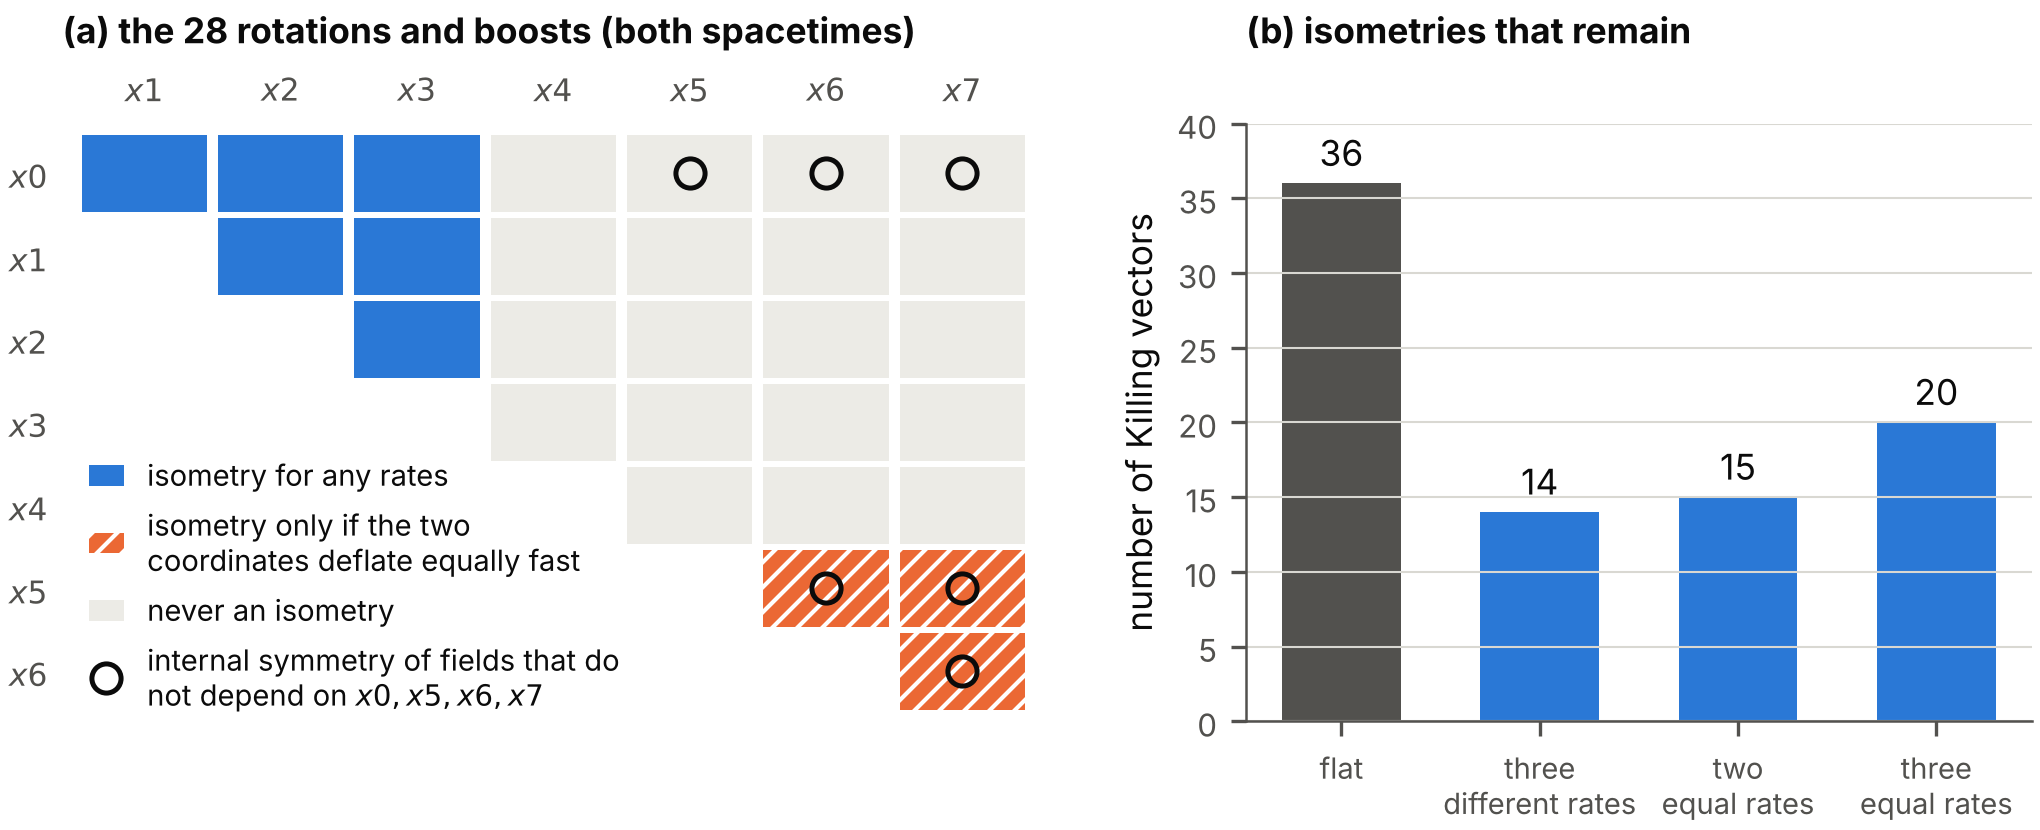
\includegraphics[width=1\textwidth,height=\textheight]{figures/fig_isometries.png}
\caption{The symmetries of the flat and of the deflating spacetimes. (a)
The 28 rotations and boosts of the flat spacetime, one square for each
pair of coordinates: those that remain isometries for any rates (the six
rotations of \(x0,x1,x2,x3\)), those that remain isometries only if the
two coordinates deflate equally fast, and those that are never
isometries of the deflating spacetime. A circle marks the six pairs
whose rotations act as internal symmetries on fields that do not depend
on \(x0,x5,x6,x7\) (Part 5). The diagram is the same for 4+4 and for
7+1. (b) Number of Killing vectors: 36 on the flat spacetime; 14, 15 and
20 on the deflating spacetime with three different, two equal and three
equal rates. Data: \texttt{data/isometries.csv}; program:
\texttt{deflation\ symmetry}.}
\end{figure}

\hypertarget{equal-rates-spaces-of-constant-curvature}{%
\subsection{1.6 Equal rates: spaces of constant
curvature}\label{equal-rates-spaces-of-constant-curvature}}

Let \(\mathrm{g55}=\mathrm{g66}=\mathrm{g77}\). Introduce four new
coordinates in place of \(x4,x5,x6,x7\):
\[\bar x4=\frac{e^{\mathrm{g55}\,x4}}{\mathrm{g55}},\qquad\bar xt=\mathrm{const}_t\,xt\quad(t=5,6,7),\]
so that \(dx4=d\bar x4/(\mathrm{g55}\,\bar x4)\). The part of the line
element that contains \(x4,\dots,x7\) becomes
\[\eta_{44}\,dx4^2-e^{-2\,\mathrm{g55}\,x4}\sum_t d\bar xt^2
=\frac{\eta_{44}\,d\bar x4^2-\sum_t d\bar xt^2}{(\mathrm{g55}\,\bar x4)^2} .\tag{1.12}\]

\begin{itemize}
\tightlist
\item
  \textbf{7+1} (\(\eta_{44}=+1\)): the line element (1.12) is that of de
  Sitter space of radius \(1/\mathrm{g55}\), in the half of its flat
  slicing in which space \emph{contracts}. De Sitter space is familiar
  as the geometry of inflation, where the same line element is used with
  the opposite direction of time. The deflating 7+1 spacetime with equal
  rates is the product of flat four-dimensional space \((x0,x1,x2,x3)\)
  with a contracting four-dimensional de Sitter space.
\item
  \textbf{4+4} (\(\eta_{44}=-1\)): the line element (1.12) is
  \emph{minus} that of four-dimensional hyperbolic space \(H^4\) of
  radius \(1/\mathrm{g55}\), in the upper-half-space form. The four
  time-like coordinates span a negative-definite space of constant
  curvature.
\end{itemize}

In both cases the Riemann tensor of the four coordinates has the form of
a space of constant curvature,
\(R_{\rho\sigma\mu\nu}=-\eta_{44}\,\mathrm{g55}^2\,(g_{\rho\mu}g_{\sigma\nu}-g_{\rho\nu}g_{\sigma\mu})\)
(checks \texttt{44d-G7}, \texttt{71d-G7}).

\emph{The three special Killing vectors.} The line element (1.12) is a
multiple of the flat one, \(\eta_{44}\,d\bar x4^2-\sum_td\bar xt^2\).
The special conformal transformations of that flat metric along the
three axes \(\bar x5,\bar x6,\bar x7\) leave the factor \(1/\bar x4^2\)
unchanged, and are therefore isometries. Their generators are, for
\(s=5,6,7\),
\[\mathcal X_{(s)}=2\,\bar xs\,\Big[\bar x4\,\frac{\partial}{\partial\bar x4}+\sum_t\bar xt\,\frac{\partial}{\partial\bar xt}\Big]
-\Big(\sum_t\bar xt^2+\eta_{44}\eta_{tt}\,\bar x4^2\Big)\frac{\partial}{\partial\bar xs},\qquad
\bar x4\,\frac{\partial}{\partial\bar x4}=\frac1{\mathrm{g55}}\,\partial_4 .\tag{1.13}\]
The sign \(\eta_{44}\eta_{tt}\) is \(+1\) for 4+4 and \(-1\) for 7+1.

\hypertarget{geodesics-what-a-classical-particle-does}{%
\subsection{1.7 Geodesics: what a classical particle
does}\label{geodesics-what-a-classical-particle-does}}

The translations give seven conserved momenta
\(P_\mu=g_{\mu\nu}\,dx^\nu/d\varsigma\), \(\mu\neq4\), where
\(\varsigma\) is an affine parameter along the path (for a massive
particle on the 7+1 spacetime, the proper time divided by the mass). The
norm of the momentum is also conserved, and gives the velocity along
\(x4\). Write \(E_\perp=\sqrt{m^2+\sum_aP_a^2}\) for the energy that the
particle would have without momentum along the deflating coordinates
(the same quantity appears for waves in Part 3). Then
\[\Big(\frac{dx4}{d\varsigma}\Big)^2=E_\perp^2\;\pm\;\sum_t\frac{P_t^2}{b_t(x4)^2},\qquad
+\ \text{for 7+1},\quad -\ \text{for 4+4}.\tag{1.14}\] The term
\(P_t^2/b_t^2\) grows as \(e^{2\,\mathrm{rate}_t\,x4}\): the conserved
momentum \(P_t\) belongs to a fixed \emph{coordinate} wavelength, and
the proper wavelength shrinks. The two spacetimes now behave in opposite
ways.

\textbf{7+1: unbounded blueshift.} The energy \(dx4/d\varsigma\) of a
particle that moves along a deflating coordinate grows without bound.
For motion along \(x5\) alone, Eq. (1.14) integrates in closed form: the
affine parameter that elapses between \(x4\) and \(x4=\infty\) is
\[\varsigma(\infty)-\varsigma(x4)=\frac{1}{\mathrm{g55}\,E_\perp}\,
\mathrm{arsinh}\Big(\frac{E_\perp\,\mathrm{const5}\,e^{-\mathrm{g55}\,x4}}{\lvert P_5\rvert}\Big),\tag{1.15}\]
which is finite. A particle with momentum along a deflating coordinate
reaches \(x4=\infty\) after a \emph{finite proper time}. The coordinates
of Eq. (1.2) do not cover its whole future: the deflating 7+1 spacetime
is geodesically incomplete. For equal rates this is the well-known fact
that the flat slicing covers only half of de Sitter space. In the
example of check \texttt{71d-G8} (\(m=1\), \(P_1=0.5\), \(P_5=0.3\),
\(\mathrm{g55}=1\), \(\mathrm{const5}=0.8\), start at \(x4=-2\)) the
proper time to \(x4=\infty\) is 3.386358.

\textbf{4+4: a turning value.} With the minus sign, the right-hand side
of Eq. (1.14) vanishes where \(\sum_tP_t^2/b_t^2=E_\perp^2\). For motion
along \(x5\) alone this happens at
\[x4_{\rm turn}=\frac{1}{\mathrm{g55}}\ln\frac{E_\perp\,\mathrm{const5}}{\lvert P_5\rvert},\tag{1.16}\]
and the affine parameter needed to reach it from \(x4\) is
\(\mathrm{arcosh}\big(E_\perp\,\mathrm{const5}\,e^{-\mathrm{g55}\,x4}/\lvert P_5\rvert\big)/(\mathrm{g55}\,E_\perp)\).
The path reaches \(x4_{\rm turn}\) and returns to smaller \(x4\). A
classical particle with momentum along a deflating \emph{time} cannot
pass the turning value of the ordinary time. In the example of check
\texttt{44d-G9} (same numbers) the turning value is 1.09240103, reached
after the affine parameter 3.38543615; the numerical integration
reproduces both.

The wave equation of Part 4 shows the same two behaviours in quantum
form: creation of particles of ever larger energy on 7+1, and total
reflection --- the extinction of the dependence on the deflating times
--- on 4+4.

\begin{figure}
\centering
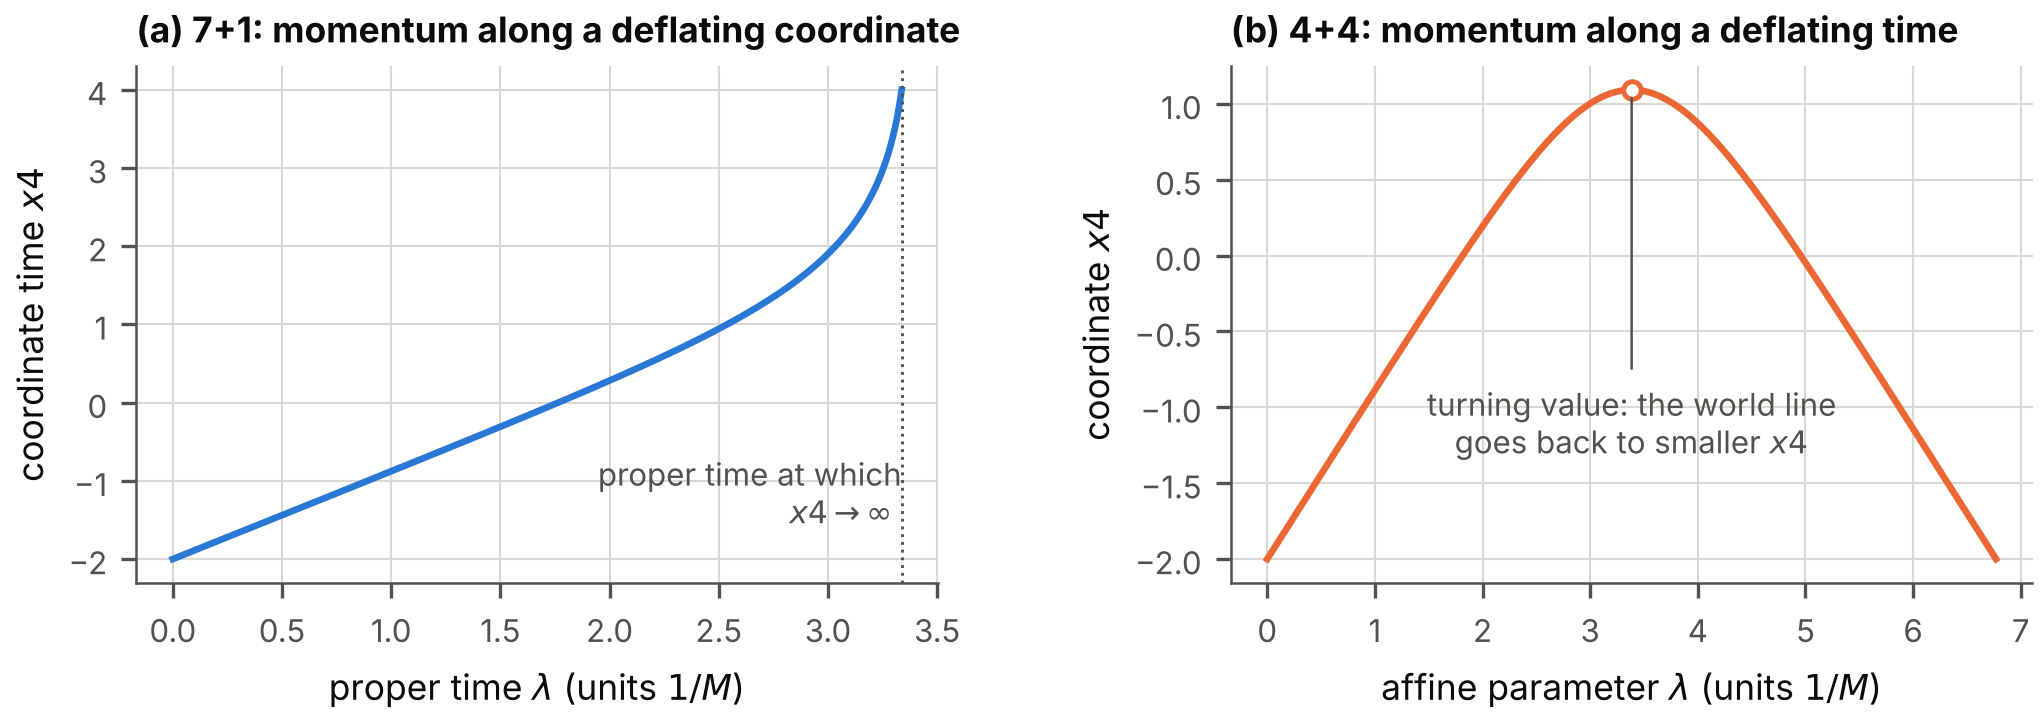
\includegraphics[width=1\textwidth,height=\textheight]{figures/fig_geodesics.png}
\caption{Geodesics with momentum along the deflating coordinate \(x5\)
(the examples of checks \texttt{71d-G8} and \texttt{44d-G9}). (a) 7+1:
the ordinary time \(x4\) against the proper time; the path runs to
\(x4=\infty\) within the finite proper time given by Eq. (1.15). (b)
4+4: \(x4\) against the affine parameter; the path turns at the value of
Eq. (1.16). Data: \texttt{data/geodesic\_1671d.csv},
\texttt{data/geodesic\_1644d.csv}; program:
\texttt{deflation\ matrices}.}
\end{figure}

\begin{center}\rule{0.5\linewidth}{0.5pt}\end{center}

\hypertarget{part-2.-dirac-matrices-and-spin-connection}{%
\section{Part 2. Dirac matrices and spin
connection}\label{part-2.-dirac-matrices-and-spin-connection}}

\hypertarget{the-matrices-of-the-frame-are-the-matrices-of-the-main-project}{%
\subsection{2.1 The matrices of the frame are the matrices of the main
project}\label{the-matrices-of-the-frame-are-the-matrices-of-the-main-project}}

At each point of a curved spacetime the tangent space is a flat space
with the metric \(\eta_{AB}\). The Dirac matrices of the orthonormal
frame are therefore the constant matrices of the flat spacetime: the
eight real 16×16 matrices \(\gamma_{1644}^A\) on the deflating 4+4
spacetime and \(\gamma_{1671}^A\) on the deflating 7+1 spacetime, with
\[\gamma^A\gamma^B+\gamma^B\gamma^A=2\,\eta^{AB}\,1 .\] Nothing about
them changes. The program of the revision nevertheless executes all 106
checks of the main project on them again, so that the revision does not
rest on a result that it has not itself verified (first part of the
command \texttt{deflation\ matrices}; Appendix A.4).

\hypertarget{the-matrices-in-coordinate-components}{%
\subsection{2.2 The matrices in coordinate
components}\label{the-matrices-in-coordinate-components}}

The Dirac matrices with a coordinate index are
\[\gamma^\mu=e_A{}^\mu\,\gamma^A:\qquad
\gamma^\mu=\gamma^{A=\mu}\ \ (\mu=0,\dots,4),\qquad
\gamma^t=\frac{1}{b_t(x4)}\,\gamma^{A=t}\ \ (t=5,6,7).\tag{2.1}\] They
are called \(\gamma_{1644d}^\mu\) and \(\gamma_{1671d}^\mu\). Five of
them are the constant matrices of the main project; the three along the
deflating coordinates are the constant matrices divided by the scale
factors, and so \emph{grow} with \(x4\). They are real, and they satisfy
the Clifford relations with the inverse of the curved metric,
\[\gamma^\mu\gamma^\nu+\gamma^\nu\gamma^\mu=2\,g^{\mu\nu}\,1,\qquad g^{tt}=\frac{\eta_{tt}}{b_t^2},\tag{2.2}\]
for all 64 pairs of indices (checks \texttt{44d-C1}, \texttt{71d-C1};
symbolically \texttt{I44d-C1}, \texttt{I71d-C1}). To avoid ambiguity, in
every formula below in which a scale factor appears explicitly the
matrices \(\gamma^4\), \(\gamma^a\), \(\gamma^t\) are the
\emph{constant} matrices of the frame.

\hypertarget{the-spin-connection}{%
\subsection{2.3 The spin connection}\label{the-spin-connection}}

\emph{Why it is needed.} A spinor is defined relative to a frame. On a
curved spacetime the frame at one point cannot be compared with the
frame at a neighbouring point without a rule, and the derivative of a
spinor must contain a term that accounts for the turning of the frame
from point to point. That term is the spin connection.

\emph{Its coefficients.} The components of the connection one-forms of
Sec. 1.3, \(\omega^A{}_B=\omega_\mu{}^A{}_B\,dx^\mu\), are given in
terms of the Christoffel symbols by the ``tetrad postulate''
\[\omega_\mu{}^A{}_B=e^A{}_\nu\big(\partial_\mu e_B{}^\nu+\Gamma^\nu{}_{\mu\lambda}\,e_B{}^\lambda\big).\tag{2.3}\]
With Eqs. (1.3), (1.5) and (1.6), and with the first index lowered,
\(\omega_{\mu AB}=\eta_{AA}\,\omega_\mu{}^A{}_B\), the only coefficients
different from zero are
\[\omega_{t\,t4}=-\omega_{t\,4t}=-\eta_{tt}\,\mathrm{rate}_t\,b_t\qquad(t=5,6,7),\tag{2.4}\]
where the first index is the coordinate index and the other two are
frame indices. For example,
\(\omega_t{}^t{}_4=e^t{}_t\,\Gamma^t{}_{t4}\,e_4{}^4=-\mathrm{rate}_t\,b_t\).
The coefficient with \(\mu=4\) vanishes because the two terms of Eq.
(2.3) cancel: \(\partial_4(1/b_t)=+\mathrm{rate}_t/b_t\) and
\(\Gamma^t{}_{4t}/b_t=-\mathrm{rate}_t/b_t\) (checks \texttt{44d-C2},
\texttt{71d-C2}; Eq. (2.4) agrees with Eq. (1.7)).

\emph{As matrices.} The spin connection acts on spinors through the
matrices \[\Omega_\mu=\tfrac14\,\omega_{\mu AB}\,\gamma^A\gamma^B:\qquad
\Omega_t=-\tfrac12\,\eta_{tt}\,\mathrm{rate}_t\,b_t\;\gamma^t\gamma^4\quad(t=5,6,7),\qquad
\Omega_0=\dots=\Omega_4=0,\tag{2.5}\] (checks \texttt{44d-C3},
\texttt{71d-C3}; symbolically \texttt{I44d-C2}, \texttt{I71d-C2}). The
covariant derivative of a spinor is
\[\nabla_\mu\psi=(\partial_\mu+\Omega_\mu)\,\psi .\] Each \(\Omega_t\)
is a multiple of the generator \(\gamma^t\gamma^4\) of the Lorentz
transformation in the plane of \(xt\) and \(x4\). On 7+1 this is a
boost, on 4+4 a rotation of two time-like directions.

\emph{The test of correctness.} The spin connection is right if and only
if the Dirac matrices are covariantly constant, that is, if
differentiating the vector index with the Christoffel symbols and the
two spinor indices with \(\Omega_\mu\) gives zero:
\[\partial_\mu\gamma^\nu+\Gamma^\nu{}_{\mu\lambda}\,\gamma^\lambda+[\Omega_\mu,\gamma^\nu]=0
\qquad\text{for all 64 pairs }(\mu,\nu),\tag{2.6}\] with the matrices
\(\gamma^\nu\) of Eq. (2.1). This is verified (checks \texttt{44d-C4},
\texttt{71d-C4}; symbolically \texttt{I44d-C3}, \texttt{I71d-C3}).
Property (2.6) is what makes the current of the Dirac field conserved
and the Dirac equation covariant.

\emph{The one combination that enters the Dirac equation.} Contracting
(2.5) with the matrices (2.1) and using \((\gamma^t)^2=\eta_{tt}\) for
the frame matrices,
\[\sum_\mu\gamma^\mu\,\Omega_\mu=-\tfrac12\sum_t\eta_{tt}\,\mathrm{rate}_t\,(\gamma^t)^2\gamma^4
=-\tfrac12\,\mathrm{gsum}\;\gamma^4 \tag{2.7}\] (checks \texttt{44d-C5},
\texttt{71d-C5}; symbolically \texttt{I44d-C4}, \texttt{I71d-C4}). The
three scale factors have cancelled, and only the total rate remains.

\hypertarget{the-curvature-of-the-spinor-derivative}{%
\subsection{2.4 The curvature of the spinor
derivative}\label{the-curvature-of-the-spinor-derivative}}

Two covariant derivatives of a spinor do not commute; their commutator
is the Riemann tensor acting on the spinor:
\[[\nabla_\mu,\nabla_\nu]\,\psi=\big(\partial_\mu\Omega_\nu-\partial_\nu\Omega_\mu+[\Omega_\mu,\Omega_\nu]\big)\psi
=\tfrac14\,R_{AB\mu\nu}\,\gamma^A\gamma^B\,\psi .\tag{2.8}\] The program
verifies this for all 64 pairs with the Riemann tensor that it computed
from the metric (checks \texttt{44d-C6}, \texttt{71d-C6}). This is a
third, independent route to the curvature, through the spinors.
Contracting once more,
\[\tfrac12\,\gamma^\mu\gamma^\nu\,[\nabla_\mu,\nabla_\nu]=-\frac R4\,1,\qquad
R=-\eta_{44}\big(\mathrm{gsq}+\mathrm{gsum}^2\big)\tag{2.9}\] (checks
\texttt{44d-C7}, \texttt{71d-C7}; symbolically \texttt{I44d-C5},
\texttt{I71d-C5}). Consequently the square of the Dirac operator
\(\gamma^\mu\nabla_\mu\) is the wave operator of the spinor derivative
minus \(R/4\): the curvature acts on a spinor like a constant addition
to the square of the mass, of magnitude
\((\mathrm{gsq}+\mathrm{gsum}^2)/4\).

\begin{center}\rule{0.5\linewidth}{0.5pt}\end{center}

\hypertarget{part-3.-the-dirac-equations-of-the-fields-dirac1671d-and-dirac1644d}{%
\section{Part 3. The Dirac equations of the fields dirac1671d and
dirac1644d}\label{part-3.-the-dirac-equations-of-the-fields-dirac1671d-and-dirac1644d}}

The Dirac equations of the main project contain the operator
\(\gamma^A\partial_A\). On a curved spacetime the partial derivative of
a spinor is replaced by the covariant derivative, and the constant
matrices by the matrices (2.1). This ``minimal'' replacement is the only
one that keeps the equation covariant and its current conserved without
introducing a new constant; it is adopted here.

\hypertarget{the-equation-of-dirac1671d}{%
\subsection{3.1 The equation of
dirac1671d}\label{the-equation-of-dirac1671d}}

The field \textbf{dirac1671d}, \(\psi_{1671d}(x)\), is a column of
sixteen complex-valued Grassmann operators on the deflating 7+1
spacetime. Its equation is
\[\boxed{\;\big(i\,\gamma_{1671d}^\mu\,\nabla_\mu-m\big)\,\psi_{1671d}=0\;}\tag{3.1}\]
With Eq. (2.7), and written with the constant matrices of the frame,
\[i\,\gamma^4\Big(\partial_4-\frac{\mathrm{gsum}}2\Big)\psi+i\sum_{a=0}^3\gamma^a\partial_a\psi
+i\sum_{t=5}^7\frac{1}{b_t(x4)}\,\gamma^t\partial_t\psi-m\,\psi=0 .\tag{3.2}\]
Compared with the flat equation (2.9) of \texttt{dirac\ matrices}, two
things have changed: the derivative along the ordinary time is shifted
by \(\mathrm{gsum}/2\), and each derivative along a deflating coordinate
is divided by its scale factor.

\hypertarget{the-equation-of-dirac1644d}{%
\subsection{3.2 The equation of
dirac1644d}\label{the-equation-of-dirac1644d}}

The field \textbf{dirac1644d}, \(\psi_{1644d}(x)\), is a column of
sixteen complex-valued Grassmann operators on the deflating 4+4
spacetime. Its equation has no factor \(i\), for the reason given in
Sec. 1.8.1 of \texttt{dirac\ matrices}:
\[\boxed{\;\big(\gamma_{1644d}^\mu\,\nabla_\mu-m\big)\,\psi_{1644d}=0\;}\tag{3.3}\]
that is,
\[\gamma^4\Big(\partial_4-\frac{\mathrm{gsum}}2\Big)\psi+\sum_{a=0}^3\gamma^a\partial_a\psi
+\sum_{t=5}^7\frac{1}{b_t(x4)}\,\gamma^t\partial_t\psi-m\,\psi=0 .\tag{3.4}\]

\hypertarget{the-weighted-field}{%
\subsection{3.3 The weighted field}\label{the-weighted-field}}

The shift of \(\partial_4\) is removed by a change of the normalization
of the field. Define the \textbf{weighted field}
\[\hat\psi=\sqrt{V_d}\;\psi .\tag{3.5}\] Because
\(\partial_4\sqrt{V_d}=-\tfrac12\,\mathrm{gsum}\,\sqrt{V_d}\) by Eq.
(1.4),
\(\sqrt{V_d}\,(\partial_4-\mathrm{gsum}/2)\,\psi=\partial_4\hat\psi\).
The weighted field therefore obeys Eqs. (3.2) and (3.4) \emph{without}
the shift:
\[\text{7+1:}\ \ \Big(i\gamma^4\partial_4+i\sum_a\gamma^a\partial_a+i\sum_t\frac{\gamma^t}{b_t}\partial_t-m\Big)\hat\psi=0,
\qquad
\text{4+4:}\ \ \Big(\gamma^4\partial_4+\sum_a\gamma^a\partial_a+\sum_t\frac{\gamma^t}{b_t}\partial_t-m\Big)\hat\psi=0 .\tag{3.6}\]

\emph{Meaning.} The quantity \(\psi^\dagger\psi\) is a number of
particles per unit of proper volume, and
\(\hat\psi^\dagger\hat\psi=V_d\,\psi^\dagger\psi\) is the number per
unit of \emph{coordinate} volume. When the deflating coordinates shrink,
the same particles occupy less proper volume and \(\psi^\dagger\psi\)
grows as \(e^{\mathrm{gsum}\,x4}\) for that reason alone. The weighted
field removes this trivial growth.

\textbf{The central observation.} \emph{A field that does not depend on
\(x5\), \(x6\), \(x7\) does not feel the deflation at all, apart from
the weight:} for such a field Eqs. (3.6) are exactly the flat equations
of the main project. Every result of the main project for fields of this
kind --- in particular, everything about the pairing of fermions ---
remains true for the weighted field. The deflation enters such results
in one way only, through the dependence of the \emph{couplings} on
\(V_d\), which the supplement RS1 derives. A field that does depend on a
deflating coordinate feels the deflation directly, through the factors
\(1/b_t\); Part 4 treats it.

\hypertarget{modes-and-the-operators-mathsf-h-and-k}{%
\subsection{\texorpdfstring{3.4 Modes, and the operators \(\mathsf h\)
and
\(K\)}{3.4 Modes, and the operators \textbackslash mathsf h and K}}\label{modes-and-the-operators-mathsf-h-and-k}}

The coefficients of Eqs. (3.6) depend on \(x4\) only. A solution can
therefore be taken proportional to
\(\exp\big(i\sum_ap_a\,xa+i\sum_tk_t\,xt\big)\), with seven constant
wavenumbers: four along the flat coordinates and three, \(k_5,k_6,k_7\),
along the deflating coordinates. (The wavenumbers along the flat
coordinates are called \(p_a\) on 7+1 and \(k_a\) on 4+4, as in the main
project. The wavenumbers \(k_t\) are called \(\kappa_t\) in
\texttt{dirac\ matrices}, where they are frequencies along the
additional times of the flat 4+4 spacetime.) A solution of this kind is
a \textbf{mode}. What remains is an ordinary differential equation in
\(x4\) for sixteen functions.

\textbf{7+1.} Multiplying the first of Eqs. (3.6) by \(\gamma^4\), with
\((\gamma^4)^2=1\), \(\beta=\gamma^4\) and
\(\alpha^A=\gamma^4\gamma^A\):
\[i\,\partial_4\hat\psi=\mathsf h(x4)\,\hat\psi,\qquad
\mathsf h(x4)=m\,\beta+\sum_{a=0}^3p_a\,\alpha^a+\sum_{t=5}^7\frac{k_t}{b_t(x4)}\,\alpha^t .\tag{3.7}\]
The matrix \(\mathsf h\) is real and symmetric for every \(x4\), and
\[\mathsf h^2=\big(E_\perp^2+k_d^2\big)\,1,\qquad
E_\perp=\sqrt{m^2+\textstyle\sum_ap_a^2},\qquad
k_d(x4)=\sqrt{\sum_t\frac{k_t^2}{b_t(x4)^2}}\tag{3.8}\] (checks
\texttt{71d-D1}, \texttt{71d-D2}; symbolically \texttt{I71d-D1}).
\(E_\perp\) is the energy that the mode would have without the deflating
coordinates. \(k_d\) is the \emph{physical} wavenumber along the
deflating coordinates; it grows with \(x4\), like
\(e^{\mathrm{rate}_t x4}\), because the coordinate wavelength
\(2\pi/k_t\) is fixed while the proper length shrinks. The evolution in
\(x4\) is unitary, and \(\hat\psi^\dagger\hat\psi\) is conserved; but
the Hamiltonian depends on the time, and its derivative
\(d\mathsf h/dx4=\sum_t\mathrm{rate}_t\,(k_t/b_t)\,\alpha^t\)
anticommutes with \(\beta\) (check \texttt{71d-D3}). A time-dependent
Hamiltonian that is not diagonal in the states of definite energy
creates pairs.

\textbf{4+4.} Multiplying the second of Eqs. (3.6) by \(\gamma^4\), with
\((\gamma^4)^2=-1\): \[\partial_4\hat\psi=K(x4)\,\hat\psi,\qquad
K(x4)=-m\,\gamma^4+i\sum_{a=0}^3k_a\,\gamma^4\gamma^a+i\sum_{t=5}^7\frac{k_t}{b_t(x4)}\,\gamma^4\gamma^t,\tag{3.9}\]
\[K^2=\big(k_d^2-E_\perp^2\big)\,1,\qquad E_\perp=\sqrt{m^2+\textstyle\sum_ak_a^2}\tag{3.10}\]
(checks \texttt{44d-D1}, \texttt{44d-D2}; symbolically
\texttt{I44d-D1}). The sign in Eq. (3.10) is the opposite of that in Eq.
(3.8), and with it the behaviour changes. While \(k_d<E_\perp\) the
square of \(K\) is negative and the mode oscillates. Once the physical
wavenumber has grown beyond \(E_\perp\) the square of \(K\) is positive,
and the solutions grow or decay exponentially (the worked example of
check \texttt{44d-D7}). The first two terms of \(K\) are anti-Hermitian
and the third is Hermitian; \(K\) is anti-Hermitian, and the evolution
unitary, if and only if \(k_5=k_6=k_7=0\) (check \texttt{44d-D5}).

The weighted field also obeys a second-order equation,
\(\partial_4^2\hat\psi=(K^2+dK/dx4)\,\hat\psi\), in which \(dK/dx4\) is
a Hermitian matrix with the square
\(\sum_t(\mathrm{rate}_t\,k_t/b_t)^2\): a Klein--Gordon equation with
one additional term that depends on the spin (check \texttt{44d-D3}).

\hypertarget{the-two-coupled-8-component-equations}{%
\subsection{3.5 The two coupled 8-component
equations}\label{the-two-coupled-8-component-equations}}

The chiral decompositions of the main project survive, because they are
properties of the frame matrices.

\textbf{4+4.} With
\(\gamma_{1644}^A=\begin{pmatrix}0&\bar\tau^A\\\tau^A&0\end{pmatrix}\)
and \(\hat\psi=(\hat\psi^L,\hat\psi^R)\), the equation of the weighted
field is the pair of real 8-component equations
\[\bar\tau^A\,e_A{}^\mu\partial_\mu\,\hat\psi^R=m\,\hat\psi^L,\qquad
\tau^A\,e_A{}^\mu\partial_\mu\,\hat\psi^L=m\,\hat\psi^R,\qquad
e_A{}^\mu\partial_\mu=\Big(\partial_0,\dots,\partial_4,\frac{\partial_5}{b_5},\frac{\partial_6}{b_6},\frac{\partial_7}{b_7}\Big)\tag{3.11}\]
(check \texttt{44d-D6}).

\textbf{7+1.} With the complex 16×8 matrices \(E^L\), \(E^R\) of the
main project and \(\hat\varphi^{L,R}=(E^{L,R})^\dagger\hat\psi\),
\[\big(i\,\partial_4+\tau^j\,e_j{}^\mu\partial_\mu\big)\hat\varphi^L=m\,\hat\varphi^R,\qquad
\big(i\,\partial_4-\tau^j\,e_j{}^\mu\partial_\mu\big)\hat\varphi^R=m\,\hat\varphi^L,\tag{3.12}\]
where \(j\) runs over the seven space-like directions \(0,1,2,3,5,6,7\)
and \(\tau^j=\tau_{1671}^j\) (check \texttt{71d-D6}).

\hypertarget{conserved-quantities-and-charge-conjugation}{%
\subsection{3.6 Conserved quantities and charge
conjugation}\label{conserved-quantities-and-charge-conjugation}}

\emph{Current.} With the adjoint \(\bar\psi=\psi^\dagger\gamma^4\) on
7+1 and \(\tilde\psi=\psi^\dagger C^-\) on 4+4, the spin connection
satisfies \(\Omega_\mu^{T}\gamma^4+\gamma^4\Omega_\mu=0\) and
\(\Omega_\mu^{T}C^-+C^-\Omega_\mu=0\) respectively (checks
\texttt{71d-C8}, \texttt{44d-C8}). Together with Eq. (2.6) this makes
the currents \(j^\mu=\bar\psi\gamma^\mu\psi\) and
\(j^\mu=\tilde\psi\gamma^\mu\psi\) of the main project conserved on the
deflating spacetimes, \(\nabla_\mu j^\mu=0\), which is the same as
\(\partial_\mu(V_d\,j^\mu)=0\): the charge is the integral of
\(V_d\,j^4\) over the seven coordinates other than \(x4\).

\emph{7+1.} \(V_d\,j^4=\hat\psi^\dagger\hat\psi\): the conserved charge
is positive, and it is the number of particles minus the number of
antiparticles after quantization, as on the flat spacetime. If \(\psi\)
is a solution then so is the charge-conjugate field
\(\omega_{1671}\psi^*\) (check \texttt{71d-D5}).

\emph{4+4.} \(V_d\,j^4=\hat\psi^\dagger W_{1644}\hat\psi\) with the
matrix \(W_{1644}=i\,C^-\gamma^4\) of the main project, which is
Hermitian, has the square one and the trace zero;
\(W_{1644}K+K^\dagger W_{1644}=0\) for all wavenumbers (check
\texttt{44d-D4}). The conserved charge of the 4+4 field is not positive,
on the deflating spacetime as on the flat one.

\begin{center}\rule{0.5\linewidth}{0.5pt}\end{center}

\hypertarget{part-4.-solutions-mode-by-mode}{%
\section{Part 4. Solutions, mode by
mode}\label{part-4.-solutions-mode-by-mode}}

\hypertarget{three-kinds-of-modes}{%
\subsection{4.1 Three kinds of modes}\label{three-kinds-of-modes}}

\begin{enumerate}
\def\labelenumi{\arabic{enumi}.}
\tightlist
\item
  \textbf{Modes that do not depend on the deflating coordinates}
  (\(k_5=k_6=k_7=0\)). By Sec. 3.3 the weighted field obeys the flat
  equation. The solutions are the plane waves of
  \texttt{dirac\ matrices}, with energies \(\pm E_\perp\), eight of each
  sign. Nothing is created and nothing is extinguished.
\item
  \textbf{Modes that depend on a deflating coordinate, early}
  (\(k_d\ll E_\perp\)). The physical wavenumber is negligible, and the
  mode behaves as in case 1.
\item
  \textbf{The same modes, late} (\(k_d\gg E_\perp\)). The physical
  wavenumber dominates. This always happens: \(k_d\) grows without
  bound, and every mode with \(k_t\neq0\) crosses from case 2 to case 3
  at the moment at which \(k_d=E_\perp\).
\end{enumerate}

The crossing is where the deflation acts. The rest of this part solves
the two equations (3.7) and (3.9) across it. Write the part of
\(\mathsf h\) and of \(K\) that contains the scale factors with the help
of one matrix,
\[\gamma^d=\frac1{k_d}\sum_{t=5}^7\frac{k_t}{b_t(x4)}\,\gamma^t,\qquad\alpha^d=\gamma^4\gamma^d:\qquad
\mathsf h=\mathsf h_\perp+k_d\,\alpha^d,\qquad K=K_\perp+i\,k_d\,\gamma^4\gamma^d,\tag{4.1}\]
where \(\mathsf h_\perp=m\beta+\sum_ap_a\alpha^a\) and
\(K_\perp=-m\gamma^4+i\sum_ak_a\gamma^4\gamma^a\) are the operators of
the modes that do not depend on the deflating coordinates. \(\gamma^d\)
is the frame matrix along the direction of the wave vector in the
deflating coordinates; \((\gamma^d)^2=-1\). The solution is exact when
\emph{one rate governs}, that is, when only one \(k_t\) differs from
zero or when the three rates are equal. In those cases \(\gamma^d\) does
not depend on \(x4\) and \(k_d(x4)\) is proportional to
\(e^{\mathrm{rate}_t\,x4}\). The natural variable is then
\[u_d=\frac{k_d(x4)}{\mathrm{rate}_t},\qquad\frac{d}{dx4}=\mathrm{rate}_t\,u_d\,\frac{d}{du_d},\tag{4.1a}\]
the physical wavenumber in units of the rate. The crossing is at
\(u_d=E_\perp/\mathrm{rate}_t\); this ratio of the energy to the rate is
the one parameter on which the results below depend.

\hypertarget{the-deflation-creates-particles}{%
\subsection{4.2 7+1: the deflation creates
particles}\label{the-deflation-creates-particles}}

\textbf{Exact solution.} Let one rate govern. In
\(\mathsf h=\mathsf h_\perp+k_d(x4)\,\alpha^d\) the two constant
matrices satisfy \(\mathsf h_\perp^2=E_\perp^2\), \((\alpha^d)^2=1\) and
\(\mathsf h_\perp\alpha^d+\alpha^d\mathsf h_\perp=0\). Let \(w\) be one
of the eight eigenvectors of \(\mathsf h_\perp\) with the eigenvalue
\(+E_\perp\); then \(\alpha^dw\) is an eigenvector with the eigenvalue
\(-E_\perp\). The ansatz \(\hat\psi=f_+(x4)\,w+i\,f_-(x4)\,\alpha^dw\)
turns Eq. (3.7) into two equations for two functions,
\[f_+'=-iE_\perp f_++k_d\,f_-,\qquad f_-'=-k_d\,f_++iE_\perp f_- .\] In
the variable \(u_d\) these are solved by Bessel functions whose orders
are \(\pm\tfrac12+iE_\perp/\mathrm{rate}_t\). Let \(Z_+\) and \(Z_-\)
denote two cylinder functions of the same kind (Bessel functions of the
first kind, of the second kind, or Hankel functions) of the orders
\(\tfrac12+iE_\perp/\mathrm{rate}_t\) and
\(-\tfrac12+iE_\perp/\mathrm{rate}_t\). The recurrence relations of the
cylinder functions connect two functions whose orders differ by one; for
this pair they read, with a prime for the derivative with respect to
\(u_d\),
\[u_d\,Z_+'=u_d\,Z_--\Big(\frac12+\frac{iE_\perp}{\mathrm{rate}_t}\Big)Z_+,\qquad
u_d\,Z_-'=-u_d\,Z_++\Big(-\frac12+\frac{iE_\perp}{\mathrm{rate}_t}\Big)Z_- .\]
With them, substitution shows that
\[\boxed{\;\hat\psi=\sqrt{u_d}\,\Big[Z_+(u_d)\;w+i\,Z_-(u_d)\;\alpha^dw\Big],\qquad
\text{orders of }Z_\pm:\ \ \pm\frac12+\frac{iE_\perp}{\mathrm{rate}_t}\;}\tag{4.2}\]
is a solution for each of the eight \(w\); two independent kinds of
cylinder function give all sixteen solutions. Check \texttt{I71d-M1}
verifies Eq. (4.2) with the Bessel functions of an arbitrary-precision
library to a relative residual of \(10^{-15}\).

\textbf{Number of created particles.} At early times (\(u_d\to0\)) a
Bessel function of the first kind behaves as the power of its argument
that its order gives. The solution that has positive energy at early
times, \(\propto e^{-iE_\perp x4}\,w\), is therefore Eq. (4.2) with the
Bessel functions of the first kind of the \emph{negative} orders:
\(Z_+\) is the function of the order
\(-\tfrac12-iE_\perp/\mathrm{rate}_t\) and \(Z_-\) is minus the function
of the order \(\tfrac12-iE_\perp/\mathrm{rate}_t\), a pair that obeys
the same recurrence relations. At late times (\(u_d\to\infty\)) the
solution of positive energy is Eq. (4.2) with the Hankel functions of
the second kind, which behave as \(e^{-iu_d}\), and the solution of
negative energy is Eq. (4.2) with the Hankel functions of the first
kind. The connection formula of the Bessel functions writes the first
solution as a sum of the other two, with coefficients of the magnitudes
\(\tfrac12e^{+\pi E_\perp/\mathrm{rate}_t}\) (for the Hankel solution of
the second kind) and \(\tfrac12e^{-\pi E_\perp/\mathrm{rate}_t}\) (first
kind). At large argument the squared magnitudes of the two Hankel
solutions themselves are \((2/\pi)\,e^{-\pi E_\perp/\mathrm{rate}_t}\)
(second kind) and \((2/\pi)\,e^{+\pi E_\perp/\mathrm{rate}_t}\) (first
kind). The weight of the negative-energy part, divided by the weight of
the positive-energy part, is therefore
\(e^{-2\pi E_\perp/\mathrm{rate}_t}\). A mode that starts empty ends
with
\[\boxed{\;n_{\rm cr}=\frac{1}{e^{2\pi E_\perp/\mathrm{rate}_t}+1}\;}\tag{4.3}\]
particles in each of its eight internal states, and with as many
antiparticles.

\emph{Meaning.} Equation (4.3) is the Fermi--Dirac distribution in the
energy \(E_\perp\) at the temperature
\[T_{\rm defl}=\frac{\mathrm{rate}_t}{2\pi}\tag{4.3a}\] (in units with
\(\hbar=k_B=1\)). For equal rates this is the Gibbons--Hawking
temperature of de Sitter space. Each mode with \(k_t\neq0\) is populated
once, at its crossing, and its particles then gain energy without bound,
\(\sqrt{E_\perp^2+k_d^2}\), as the classical particle of Sec. 1.7 does.
Modes with \(k_t=0\) stay empty.

\textbf{Numerical verification.} The program integrates Eq. (3.7) for
all sixteen components through the crossing and projects the result on
the states of negative energy.

\begin{itemize}
\tightlist
\item
  \emph{One direction} (check \texttt{71d-M1}): for
  \(E_\perp/\mathrm{g55}=0.25,0.5,\dots,3.0\) the created number agrees
  with Eq. (4.3) to a relative deviation of at most
  \(3.2\times10^{-6}\), while the numbers themselves range from 0.17 to
  \(6.5\times10^{-9}\); the eight internal states are created equally.
\item
  \emph{Equal rates, all three directions} (check \texttt{71d-M2}): for
  a mode with \((k_5,k_6,k_7)=(0.5,-0.8,0.3)\) and three different
  constants the created number is \(5.70627486\times10^{-3}\) in all
  eight states, and Eq. (4.3) gives \(5.70627482\times10^{-3}\). With
  equal rates the result depends neither on the direction of the
  wavenumber nor on the constants.
\item
  \emph{Unequal rates} (check \texttt{71d-M3}): no exact solution is
  known. If the second physical wavenumber is still below
  \(e^{-3}E_\perp\) at the moment at which the first reaches
  \(E_\perp\), the mean created number is Eq. (4.3) with the rate of the
  coordinate that becomes energetic first, to within 1.2 per cent. If
  two directions become energetic together, the eight internal states
  are created \emph{unequally} --- in the cases computed, by up to a
  factor 110 between the most and the least populated state --- and the
  result is known only numerically
  (\texttt{data/creation\_anisotropic.csv}).
\item
  \emph{Independent integration} (checks \texttt{I71d-M2},
  \texttt{I71d-M3}): a Runge--Kutta method of a general-purpose library
  reproduces Eq. (4.3) to \(2\times10^{-5}\).
\end{itemize}

\begin{figure}
\centering
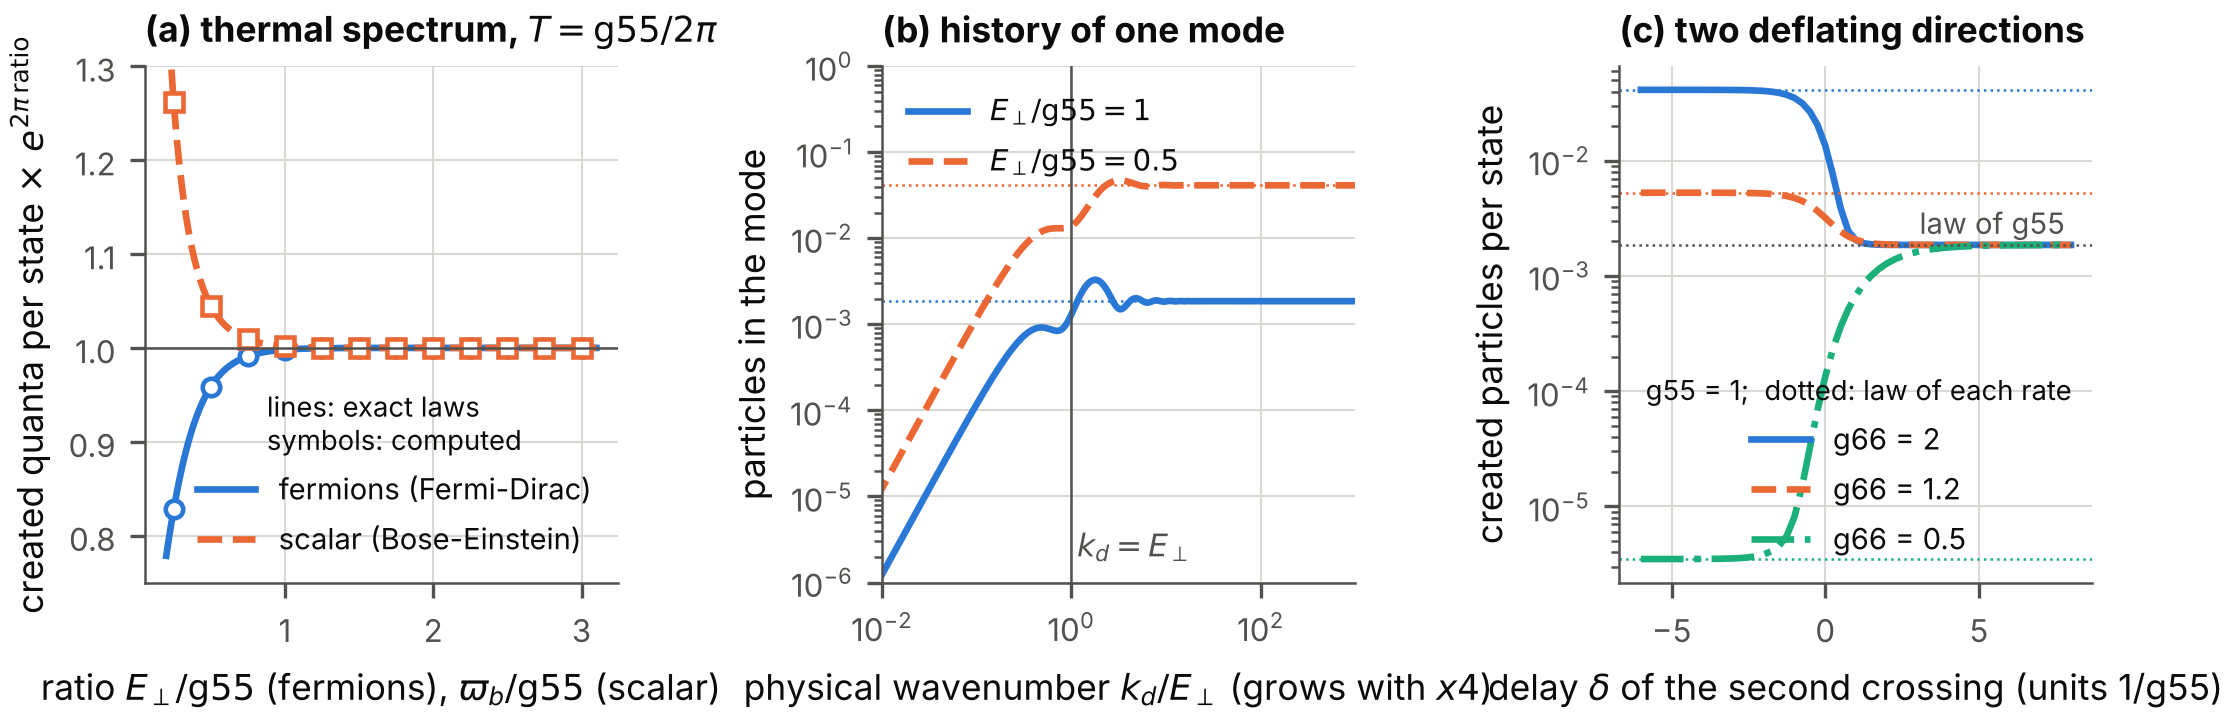
\includegraphics[width=1\textwidth,height=\textheight]{figures/fig_creation.png}
\caption{Creation of particles on the deflating 7+1 spacetime. (a)
Created quanta per state, multiplied by \(e^{2\pi\,\mathrm{ratio}}\),
against the ratio of the energy to the rate: fermions follow the
Fermi--Dirac law (4.3), the scalar modes of the supplement RS1 the
Bose--Einstein law, both at the temperature \(\mathrm{g55}/2\pi\).
Lines: the exact laws; symbols: computed. (b) History of two modes, with
\(E_\perp/\mathrm{g55}=1\) and \(0.5\): the number of particles in the
mode against the physical wavenumber \(k_d/E_\perp\), which grows with
the time; after the crossing at \(k_d=E_\perp\) the number settles at
the value of Eq. (4.3) (dotted). (c) Two deflating directions,
\(\mathrm{g55}=1\) and \(\mathrm{g66}=2\), \(1.2\) or \(0.5\): mean
number of created particles per state against the delay between the two
crossings; the dotted lines are Eq. (4.3) with each of the rates. Data:
\texttt{data/creation\_single.csv}, \texttt{data/boson\_creation.csv},
\texttt{data/creation\_history.csv},
\texttt{data/creation\_anisotropic.csv}; programs:
\texttt{deflation\ modes}, \texttt{deflation\ channels}.}
\end{figure}

\hypertarget{the-deflation-extinguishes-the-dependence-on-the-deflating-times}{%
\subsection{4.3 4+4: the deflation extinguishes the dependence on the
deflating
times}\label{the-deflation-extinguishes-the-dependence-on-the-deflating-times}}

\textbf{Exact solution.} Let one rate govern. In
\(K=K_\perp+i\,k_d(x4)\,\gamma^4\gamma^d\) the first matrix is
anti-Hermitian with \(K_\perp^2=-E_\perp^2\); the matrix
\(i\gamma^4\gamma^d\) is Hermitian with the square one; and the two
anticommute. Let \(w\) be one of the eight eigenvectors of \(K_\perp\)
with the eigenvalue \(+iE_\perp\); then \(i\gamma^4\gamma^dw\) has the
eigenvalue \(-iE_\perp\) and is orthogonal to \(w\). The ansatz
\(\hat\psi=f_+\,w+f_-\,i\gamma^4\gamma^dw\) gives
\[f_+'=iE_\perp f_++k_d\,f_-,\qquad f_-'=k_d\,f_+-iE_\perp f_- .\] These
are solved by the modified Bessel functions that decay at large
argument, of the orders \(\tfrac12\mp iE_\perp/\mathrm{rate}_t\). Such a
function is written with its order as a subscript and with an argument;
the letter \(K\) without subscript and argument is the matrix of Eq.
(3.9). The recurrence relation for this pair of orders is
\[u_d\,K_{1/2-iE_\perp/\mathrm{rate}_t}'=-u_d\,K_{1/2+iE_\perp/\mathrm{rate}_t}
-\Big(\frac12-\frac{iE_\perp}{\mathrm{rate}_t}\Big)K_{1/2-iE_\perp/\mathrm{rate}_t},\]
together with the relation obtained from it by reversing the sign of
\(i\). With them, substitution shows that
\[\boxed{\;\hat\psi=\sqrt{u_d}\,\Big[K_{1/2-iE_\perp/\mathrm{rate}_t}(u_d)\;w
-K_{1/2+iE_\perp/\mathrm{rate}_t}(u_d)\;i\gamma^4\gamma^dw\Big]\;}\tag{4.4}\]
is a solution for each of the eight \(w\) (check \texttt{I44d-M1},
relative residual \(10^{-15}\)). The other eight solutions are built in
the same way from the modified Bessel functions that \emph{grow} as
\(e^{+u_d}\).

\textbf{The bounded solutions.} Since \(u_d\) itself grows exponentially
with \(x4\), a solution of the second kind grows as the exponential of
an exponential. Such a solution is not admissible: it is the analogue of
the growing exponential under a potential barrier. Admissible are the
eight solutions (4.4), which stay bounded. Their properties are exact.

\begin{itemize}
\tightlist
\item
  \emph{Magnitude.} Because \(w\) and \(i\gamma^4\gamma^dw\) are
  orthogonal, and because the two functions in Eq. (4.4) are complex
  conjugates of each other for real argument,
  \[\lvert\hat\psi\rvert^2=2\,u_d\,\big\lvert K_{1/2+iE_\perp/\mathrm{rate}_t}(u_d)\big\rvert^2\,\lvert w\rvert^2 .\tag{4.5}\]
  The numerical integration reproduces Eq. (4.5) over the range
  \(0.02<u_d<12\) to a relative deviation of \(3.6\times10^{-12}\)
  (check \texttt{44d-M4}).
\item
  \emph{Early times} (\(u_d\to0\)):
  \(\lvert\hat\psi\rvert^2\to\pi\,\lvert w\rvert^2/\cosh(\pi E_\perp/\mathrm{rate}_t)\),
  a constant. The solution is then a combination of
  \(e^{+iE_\perp x4}\,w\) and \(e^{-iE_\perp x4}\,i\gamma^4\gamma^dw\)
  with coefficients of \emph{equal} magnitude: the two signs of the
  frequency enter with equal weight. A bounded solution is a
  \textbf{standing wave} in the ordinary time, not a travelling wave
  (check \texttt{44d-M1}: the parts of positive and of negative energy
  have equal weight to \(2\times10^{-14}\)). Its conserved charge
  \(\hat\psi^\dagger W\hat\psi\) vanishes (check \texttt{44d-M2}).
\item
  \emph{Late times} (\(u_d\to\infty\)):
  \(\lvert\hat\psi\rvert^2\to\pi\,\lvert w\rvert^2\,e^{-2u_d}\). The
  mode dies out as the exponential of an exponential of the time.
\end{itemize}

\textbf{The law of the extinction.} In the semiclassical (WKB)
approximation the bounded solution falls beyond the turning value
\(x4_{\rm turn}\), at which \(k_d=E_\perp\), as \(e^{-S_{\rm WKB}}\)
with \[S_{\rm WKB}=\int_{x4_{\rm turn}}^{x4}\sqrt{k_d^2-E_\perp^2}\;dx4'
=\frac{1}{\mathrm{rate}_t}\Big[\sqrt{k_d^2-E_\perp^2}-E_\perp\arccos\frac{E_\perp}{k_d}\Big]
\ \longrightarrow\ \frac{k_d-\tfrac{\pi}{2}E_\perp}{\mathrm{rate}_t}\quad(k_d\gg E_\perp).\]
The exact solution (4.5) fixes the constant that the approximation
leaves open:
\[\ln\frac{\lvert\hat\psi\rvert_{\rm early}}{\lvert\hat\psi\rvert_{\rm late}}-S_{\rm WKB}
\ \longrightarrow\ \tfrac12\ln2-\tfrac12\ln\big(1+e^{-2\pi E_\perp/\mathrm{rate}_t}\big).\tag{4.6}\]
The numerical integration confirms Eq. (4.6) to \(3.6\times10^{-4}\) in
the four cases in which one rate governs; with three unequal rates the
constant depends on the internal state, with a spread of 0.40 at
\(S_{\rm WKB}=30\) (check \texttt{44d-M3}). The independent script
confirms Eq. (4.6) with the Bessel functions of another library (check
\texttt{I44d-M2}).

\emph{Meaning.} On the flat 4+4 spacetime a field that depends on the
additional times evolves non-unitarily in the ordinary time, which is
the principal difficulty of four time-like dimensions (Sec. 1.8.4 of
\texttt{dirac\ matrices}). On the deflating 4+4 spacetime every
admissible mode that depends on a deflating time is a standing wave that
is extinguished after its crossing, with \(S_{\rm WKB}\) growing as
\(e^{\mathrm{rate}_t\,x4}\). What remains at late times is the sector of
fields that do not depend on \(x5\), \(x6\), \(x7\) --- and in that
sector the evolution is unitary and \(\hat\psi^\dagger\hat\psi\) is
conserved (check \texttt{44d-D5}). The deflation of the three additional
times thus removes, dynamically, the sector that causes the difficulty.
The classical counterpart is the turning value of Sec. 1.7. Part 6
states the limits of this conclusion.

\begin{figure}
\centering
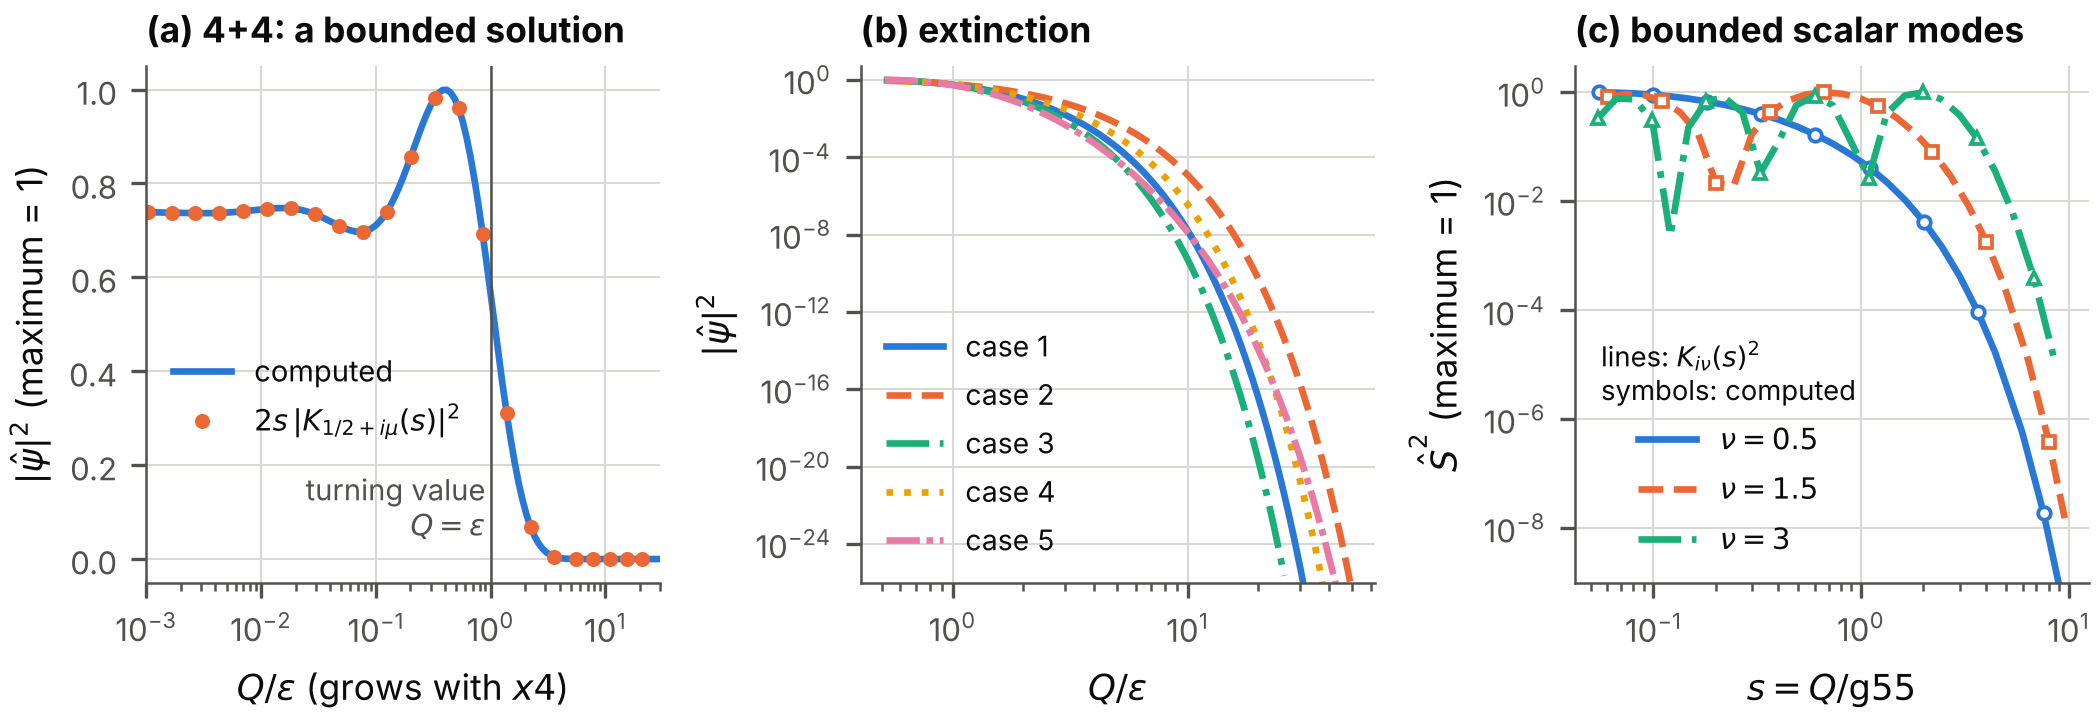
\includegraphics[width=1\textwidth,height=\textheight]{figures/fig_extinction.png}
\caption{Extinction on the deflating 4+4 spacetime. (a) A bounded
solution: \(\lvert\hat\psi\rvert^2\) against the physical wavenumber
\(k_d/E_\perp\), which grows with the time; computed (line) and the
exact form (4.5) (symbols). It is constant long before the crossing at
\(k_d=E_\perp\) and falls after it. (b) The five cases of check
\texttt{44d-M3} on a logarithmic scale. (c) The bounded modes of a
scalar field on the same spacetime (supplement RS1), which are
extinguished in the same way; lines: exact, symbols: computed. Data:
\texttt{data/extinction\_profile.csv},
\texttt{data/extinction\_checks.csv}, \texttt{data/boson\_bounded.csv};
programs: \texttt{deflation\ modes}, \texttt{deflation\ channels}.}
\end{figure}

\hypertarget{the-numerical-method-and-its-tests}{%
\subsection{4.4 The numerical method and its
tests}\label{the-numerical-method-and-its-tests}}

Equations (3.7) and (3.9) are linear equations with coefficients that
grow exponentially, and a general-purpose integrator with a fixed step
fails on them. The program uses a commutator-free Magnus method of order
four: over each step the solution is advanced by the product of two
matrix exponentials of linear combinations of the coefficient matrix at
two Gauss points. Because \(\mathsf h^2\) and \(K^2\) are multiples of
the unit matrix at any one time, each exponential is evaluated in closed
form (a cosine and a sine, or their hyperbolic counterparts), and for
\(\mathsf h\) every step is exactly unitary. The length of each step is
chosen so that neither the phase accumulated in the step nor the
relative change of the coefficients exceeds a fixed bound; the steps
therefore shorten as the coefficients grow.

\emph{Reading off the number of particles.} At a finite time the state
of positive energy of the instantaneous Hamiltonian is not yet the state
of a free particle, because the Hamiltonian still changes. The program
projects instead on the eigenstates of the first ``superadiabatic''
Hamiltonian, which is \(\mathsf h\) corrected by a term of the first
order in the rate at which the direction of \(\mathsf h\) changes (the
formula is in the documentation of the function
\texttt{negative\_projector} of \texttt{modes.rs}). This removes the
leading spurious oscillation of the particle number. The error that
remains decreases as the final value of \(k_d/E_\perp\) is increased,
and is contained in the deviations quoted above.

\emph{Tests.} The unit tests of the modules \texttt{modes} and
\texttt{scalar} (run by \texttt{cargo\ test}) verify the order of
convergence of the method, the unitarity of every step, the agreement
with Eq. (4.3) and with Eq. (4.5), and the modified Bessel function of
complex order, which the program computes from its integral
representation. The independent script uses different tools throughout:
an explicit Runge--Kutta method of order eight and the Bessel functions
of an arbitrary-precision library.

\begin{center}\rule{0.5\linewidth}{0.5pt}\end{center}

\hypertarget{part-5.-which-symmetries-of-the-flat-spacetimes-survive}{%
\section{Part 5. Which symmetries of the flat spacetimes
survive}\label{part-5.-which-symmetries-of-the-flat-spacetimes-survive}}

\textbf{Rotations and boosts.} The flat spacetimes have 28 rotations and
boosts, one for each pair of coordinates. The program tests each of the
28 on the deflating spacetime (checks \texttt{44d-S1}, \texttt{71d-S1}):

\begin{itemize}
\tightlist
\item
  the 6 rotations of \(x0,x1,x2,x3\) survive for any rates;
\item
  the rotation of two deflating coordinates survives if and only if
  their rates are equal (in the form given in Sec. 1.5, which contains
  the two constants);
\item
  nothing that involves \(x4\) survives --- on 7+1 these are the seven
  boosts, among them the three boosts of ordinary special relativity
  along \(x1,x2,x3\);
\item
  nothing that mixes \(x0\), or any flat coordinate, with a deflating
  coordinate survives.
\end{itemize}

That the boosts along \(x1,x2,x3\) are no longer symmetries deserves a
remark. The deflation defines a preferred state of rest, as the
expansion of the universe does: the frame in which the scale factors
depend on the time alone and not on the position. For fields that do not
depend on \(x5,x6,x7\) the flat equations hold for the weighted field
(Sec. 3.3), and their solutions are related by the ordinary boosts as
before. What singles out the preferred frame for such fields is only the
dependence of the couplings on \(x4\) (supplement RS1).

\textbf{The internal symmetry of fields that do not depend on the extra
coordinates.} The main project found that the eight internal states of
the fermion, for fields that depend on \(x1,x2,x3,x4\) only, carry the
symmetry \(su(2)_A\oplus su(2)_B\oplus u(1)_F\oplus u(1)_E\). Because
the weighted field of this sector obeys the flat equations, the symmetry
is unchanged by the deflation (check \texttt{def-S3}). Six of its
generators are the products \(\gamma^A\gamma^B\) of the six pairs taken
from the four axes \(x0,x5,x6,x7\); on the flat spacetime they are
rotations of these axes. On the deflating spacetime 0, 1 or 3 of the six
are still isometries, for three different, two equal or three equal
rates (checks \texttt{44d-S2}, \texttt{71d-S2}). The others remain exact
symmetries of the sector \emph{without} being symmetries of the
spacetime. The supplement RS2 examines what this means for the
hypothesis about the Higgs field.

\textbf{Discrete symmetries.} The scale factors are real and depend on
\(x4\) only. Reflections of any coordinate other than \(x4\) and charge
conjugation (check \texttt{71d-D5}) survive. The reversal of the
ordinary time does not: it turns deflation into inflation.

\begin{center}\rule{0.5\linewidth}{0.5pt}\end{center}

\hypertarget{part-6.-what-has-been-established-and-what-has-not}{%
\section{Part 6. What has been established, and what has
not}\label{part-6.-what-has-been-established-and-what-has-not}}

\textbf{Established} (each item by exact arithmetic at rational
parameters and, where marked with I, symbolically for arbitrary
parameters).

\begin{enumerate}
\def\labelenumi{\arabic{enumi}.}
\tightlist
\item
  The geometry of the two deflating spacetimes: Christoffel symbols,
  Riemann and Ricci tensors, curvature scalar and Einstein tensor in
  closed form (I); the Killing vectors, 14, 15 or 20, and the
  completeness of the lists; homogeneity; constant curvature of the four
  coordinates \(x4,\dots,x7\) for equal rates.
\item
  The deflating spacetimes are not vacuum solutions of Einstein's
  equations, with or without a cosmological constant.
\item
  Geodesics: unbounded blueshift and geodesic incompleteness on 7+1; a
  turning value of the ordinary time on 4+4.
\item
  The Dirac matrices in coordinate components, the spin connection, the
  covariant constancy of the matrices, and the curvature of the spinor
  derivative (I).
\item
  The Dirac equations (3.1) and (3.3); the weighted field; the statement
  that fields independent of \(x5,x6,x7\) obey the flat equations; the
  operators \(\mathsf h\) and \(K\) and their squares (I); the
  8-component forms; the conserved currents.
\item
  The exact solutions (4.2) and (4.4) when one rate governs, the law of
  creation (4.3) on 7+1, and the standing waves and the law of
  extinction (4.5), (4.6) on 4+4; all confirmed numerically by two
  independent methods.
\item
  Which rotations and boosts survive, and that the internal symmetry of
  the sector of fields independent of the extra coordinates does not
  change.
\end{enumerate}

\textbf{Not established.}

\begin{enumerate}
\def\labelenumi{\arabic{enumi}.}
\tightlist
\item
  \emph{The source of the deflation.} The hypotheses prescribe the
  metric. No field equation for the metric has been solved, and the
  stress tensor that Eq. (1.10) would require has not been identified
  with any matter. All results here are results on a prescribed
  background.
\item
  \emph{The effect of the fields on the metric.} The particles created
  on 7+1 gain energy without bound. Their stress tensor must eventually
  change the metric; this back-reaction has not been computed, and the
  results for 7+1 hold only for as long as it can be neglected.
\item
  \emph{The future boundary of 7+1.} The coordinates do not cover the
  whole future of the particles that move along deflating coordinates
  (Sec. 1.7). What lies beyond is outside the hypotheses.
\item
  \emph{The exclusion of the growing solutions on 4+4.} The eight
  growing solutions are discarded because they are unbounded. That is a
  condition of admissibility, imposed as in the theory of a barrier; it
  is not derived from a principle, and the 4+4 theory still has no
  positive conserved charge for modes that depend on the deflating
  times. The statement of Sec. 4.3 is that the admissible modes die out,
  not that the difficulty of the four time-like dimensions has been
  solved.
\item
  \emph{Unequal rates with simultaneous crossings.} No closed form is
  known; the results are numerical.
\item
  \emph{Quantization on 4+4.} As in the main project, a consistent
  quantization of the 4+4 field exists only for the sector that does not
  depend on the additional times.
\end{enumerate}

\begin{center}\rule{0.5\linewidth}{0.5pt}\end{center}

\hypertarget{appendix-a.-complete-output-of-the-programs}{%
\section{Appendix A. Complete output of the
programs}\label{appendix-a.-complete-output-of-the-programs}}

In all files ``exact'' means that the statement is an identity verified
in exact rational arithmetic, and ``numerical'' that it involves real
numbers and is verified to the accuracy stated in the line.

\hypertarget{a.1-geometry-matrices-spin-connection-dirac-operators}{%
\subsection{A.1 Geometry, matrices, spin connection, Dirac
operators}\label{a.1-geometry-matrices-spin-connection-dirac-operators}}

The file \texttt{data/deflating\_checks.txt}, written by
\texttt{deflation\ matrices}:

\begin{Shaded}
\begin{Highlighting}[]
\NormalTok{PROJECT spacetimes, Revision\_Deflation: checks of the geometry, of the Dirac matrices, of the spin connection and of the Dirac operators of the deflating spacetimes (44d{-}..: 4+4 with deflating x5, x6, x7; 71d{-}..: 7+1 with deflating x5, x6, x7)}
\NormalTok{generated by: deflation (Rust crate spacetimes{-}deflation, version 0.1.0; PROJECT spacetimes, Revision\_Deflation); command: deflation matrices}
\NormalTok{45 of 45 checks passed}

\NormalTok{[PASS] 44d{-}G1  (exact) metric of the deflating 4+4 spacetime: g\_1644d = diag(eta\_00, .., eta\_44, eta\_55 b\_5\^{}2, eta\_66 b\_6\^{}2, eta\_77 b\_7\^{}2) with eta = diag[1, 1, 1, 1, {-}1, {-}1, {-}1, {-}1] and the scale factors b\_5 = const5 exp({-}g55 x4), b\_6 = const6 exp({-}g66 x4), b\_7 = const7 exp({-}g77 x4), that is g\_55 = {-}const5\^{}2 exp({-}2 g55 x4) and likewise g\_66, g\_77 (the author\textquotesingle{}s formulas; g55, g66, g77 \textgreater{} 0 are the three rates, and in statements with a general index t = 5, 6, 7 the rate of xt is written rate\_t, gsum = g55 + g66 + g77). Verified: g\_tt = {-}b\_t\^{}2 and d g\_tt/dx4 = {-}2 rate\_t g\_tt; the frame e\^{}A = (dx0, .., dx4, b\_5 dx5, b\_6 dx6, b\_7 dx7) is orthonormal. All exact geometry checks use five rational parameter sets: (g55, g66, g77) = (1, 1, 1) at a point where (b\_5, b\_6, b\_7) = (1, 1, 1); (g55, g66, g77) = (1, 2, 3) at a point where (b\_5, b\_6, b\_7) = (1/2, 1/3, 1/5); (g55, g66, g77) = (1/2, 3/4, 5/3) at a point where (b\_5, b\_6, b\_7) = (2, 1/3, 5/7); (g55, g66, g77) = (2, 2, 5) at a point where (b\_5, b\_6, b\_7) = (3/2, 3/2, 1/4); (g55, g66, g77) = (7/3, 7/3, 7/3) at a point where (b\_5, b\_6, b\_7) = (1/2, 3, 5/4)}
\NormalTok{[PASS] 44d{-}G2  (exact) the Christoffel symbols computed from their definition are Gamma\^{}t\_(4t) = Gamma\^{}t\_(t4) = {-}rate\_t and Gamma\^{}4\_(tt) = eta\_44 eta\_tt rate\_t b\_t\^{}2 (t = 5, 6, 7); all others vanish}
\NormalTok{[PASS] 44d{-}G3  (exact) Cartan\textquotesingle{}s structure equations hold with the spin{-}connection coefficients of the tetrad postulate: the torsion d e\^{}A + omega\^{}A\_B \^{} e\^{}B vanishes, and d omega\^{}A\_B + omega\^{}A\_C \^{} omega\^{}C\_B equals the Riemann tensor computed from the Christoffel symbols (two independent routes to the curvature)}
\NormalTok{[PASS] 44d{-}G4  (exact) Riemann tensor in the orthonormal frame: R\^{}t\_(4t4) = {-}rate\_t\^{}2, R\^{}4\_(t4t) = {-}eta\_44 eta\_tt rate\_t\^{}2, R\^{}t\_(sts) = {-}eta\_44 eta\_ss rate\_t rate\_s (t != s in \{5, 6, 7\}), and the components that follow from antisymmetry; all other components vanish. No component involves x0, x1, x2 or x3: the space of these four coordinates is flat}
\NormalTok{[PASS] 44d{-}G5  (exact) with gsq = g55\^{}2 + g66\^{}2 + g77\^{}2 and gsum = g55 + g66 + g77: Ricci tensor R\^{}4\_4 = {-}eta\_44 gsq, R\^{}t\_t = {-}eta\_44 rate\_t gsum, R\^{}a\_a = 0 (a = 0..3); curvature scalar R = {-}eta\_44 (gsq + gsum\^{}2); Einstein tensor G\^{}4\_4 = eta\_44 (g55 g66 + g55 g77 + g66 g77), G\^{}t\_t = eta\_44 [(gsq + gsum\^{}2)/2 {-} rate\_t gsum], G\^{}a\_a = eta\_44 (gsq + gsum\^{}2)/2; its covariant divergence vanishes. The Einstein tensor does not vanish: the deflating spacetime is not a vacuum solution of Einstein\textquotesingle{}s equations}
\NormalTok{[PASS] 44d{-}G6  (exact) Killing vectors (the Lie derivative of the metric along each vanishes identically): 7 translations (x0, x1, x2, x3, x5, x6, x7), 6 rotations of (x0, x1, x2, x3), and the scaling d/dx4 + sum\_t rate\_t xt d/dxt, 14 in all; one more for every pair of equal rates (a rotation of the two coordinates); and 20 in all if the three rates are equal. Numbers found for the five parameter sets: [20, 14, 14, 15, 20]}
\NormalTok{[PASS] 44d{-}G7  (exact) if the three rates are equal, g55 = g66 = g77, the part (x4, x5, x6, x7) of the metric has constant curvature, R\_(rho sigma mu nu) = +g55\^{}2 (g\_(rho mu) g\_(sigma nu) {-} g\_(rho nu) g\_(sigma mu)): the four time{-}like coordinates carry minus the metric of hyperbolic space H\^{}4 of radius 1/g55, written in horospherical coordinates}
\NormalTok{[PASS] 44d{-}G9  (numerical) geodesic with m = 1, momentum P\_1 = 0.5 along x1 and P\_5 = 0.3 along the deflating time x5 (g55 = 1, const5 = 0.8), started at x4 = {-}2 with increasing x4: P\_1, P\_5 and the norm are conserved to 1.7e{-}14; the path reaches the largest value x4 = 1.09240103 (predicted turning value ln(E\_perp const5/|P\_5|)/g55 with E\_perp = sqrt(m\^{}2 + P\_1\^{}2) = 1.09240103) after the affine parameter 3.38543615 (closed form 3.38543615) and then returns to smaller x4: a particle with momentum along a deflating time cannot pass the turning value}
\NormalTok{[PASS] 44d{-}C1  (exact) the coordinate matrices gamma\_1644d\^{}mu = e\_A\^{}mu gamma1644[A] (gamma\^{}t = gamma1644[t]/b\_t for t = 5, 6, 7; the other five unchanged) are real and satisfy gamma\^{}mu.gamma\^{}nu + gamma\^{}nu.gamma\^{}mu = 2 g\_1644d\^{}(mu nu) 1 for all 64 pairs, with g\^{}(tt) = eta\^{}(tt)/b\_t\^{}2. Verified for five rational parameter sets: (g55, g66, g77) = (1, 1, 1) at a point where (b\_5, b\_6, b\_7) = (1, 1, 1); (g55, g66, g77) = (1, 2, 3) at a point where (b\_5, b\_6, b\_7) = (1/2, 1/3, 1/5); (g55, g66, g77) = (1/2, 3/4, 5/3) at a point where (b\_5, b\_6, b\_7) = (2, 1/3, 5/7); (g55, g66, g77) = (2, 2, 5) at a point where (b\_5, b\_6, b\_7) = (3/2, 3/2, 1/4); (g55, g66, g77) = (7/3, 7/3, 7/3) at a point where (b\_5, b\_6, b\_7) = (1/2, 3, 5/4)}
\NormalTok{[PASS] 44d{-}C2  (exact) the spin{-}connection coefficients computed from the tetrad postulate omega\_mu\^{}A\_B = e\^{}A\_nu (d\_mu e\_B\^{}nu + Gamma\^{}nu\_(mu lam) e\_B\^{}lam), with the Christoffel symbols obtained from the metric, are antisymmetric, omega\_(mu A B) = {-}omega\_(mu B A), and the only non{-}zero ones are omega\_(t,t4) = {-}omega\_(t,4t) = {-}eta\_tt rate\_t b\_t (t = 5, 6, 7); same five parameter sets}
\NormalTok{[PASS] 44d{-}C3  (exact) Omega\_mu := (1/4) omega\_(mu A B) gamma1644[A].gamma1644[B] equals {-}(1/2) eta\_tt rate\_t b\_t gamma1644[t].gamma1644[4] for mu = t in \{5, 6, 7\} and vanishes for mu = 0..4: the spin connection is an element of the Lie algebra spanned by the scaled commutators Sigma\^{}(t4)}
\NormalTok{[PASS] 44d{-}C4  (exact) d\_mu gamma\^{}nu + Gamma\^{}nu\_(mu lam) gamma\^{}lam + [Omega\_mu, gamma\^{}nu] = 0 for all 64 pairs (mu, nu), with d\_4 gamma\^{}t = +rate\_t gamma\^{}t: the coordinate matrices are covariantly constant}
\NormalTok{[PASS] 44d{-}C5  (exact) sum\_mu gamma\^{}mu.Omega\_mu = {-}(1/2) (g55 + g66 + g77) gamma1644[4]: in the Dirac operator the spin connection amounts to the replacement d\_4 {-}\textgreater{} d\_4 {-} gsum/2, which the weighted field psihat = sqrt(b\_5 b\_6 b\_7) psi removes}
\NormalTok{[PASS] 44d{-}C6  (exact) d\_mu Omega\_nu {-} d\_nu Omega\_mu + [Omega\_mu, Omega\_nu] = (1/4) R\_(A B mu nu) gamma1644[A].gamma1644[B] for all 64 pairs (mu, nu), with the Riemann tensor that metric.rs computes from the metric (d\_4 Omega\_t = {-}rate\_t Omega\_t): the curvature of the spinor derivative is the Riemann tensor}
\NormalTok{[PASS] 44d{-}C7  (exact) (1/2) sum\_(mu nu) gamma\^{}mu.gamma\^{}nu.(d\_mu Omega\_nu {-} d\_nu Omega\_mu + [Omega\_mu, Omega\_nu]) = {-}(R/4) 1 with the curvature scalar R = {-}eta\_44 (g55\^{}2 + g66\^{}2 + g77\^{}2 + gsum\^{}2): the square of the Dirac operator differs from the wave operator of the spinor derivative by {-}R/4}
\NormalTok{[PASS] 44d{-}C8  (exact) transpose(Omega\_mu).Cm1644 + Cm1644.Omega\_mu = 0 (Cm1644 = gamma1644[0].gamma1644[1].gamma1644[2].gamma1644[3]): the adjoint field psi\^{}dagger Cm1644 is differentiated with {-}Omega\_mu on its right, as the conserved current requires}
\NormalTok{[PASS] 44d{-}D1  (exact) in momentum space (d\_mu {-}\textgreater{} i k\_mu) the Dirac operator of the weighted field at fixed x4, D = i gamma\^{}mu k\_mu with the coordinate matrices, satisfies (D + m)(D {-} m) = {-}(g\^{}(mu nu) k\_mu k\_nu + m\^{}2) 1 with g\^{}(mu nu) k\_mu k\_nu = k\_0\^{}2 + k\_1\^{}2 + k\_2\^{}2 + k\_3\^{}2 {-} k\_4\^{}2 {-} sum\_t k\_t\^{}2/b\_t\^{}2: the instantaneous mass shell is k\_4\^{}2 + sum\_t k\_t\^{}2/b\_t(x4)\^{}2 = |k|\^{}2 + m\^{}2. Verified for five rational parameter sets and four rational momenta each}
\NormalTok{[PASS] 44d{-}D2  (exact) the generator of the evolution of the weighted field in x4, K(x4) = {-}m gamma1644[4] + i sum\_a k\_a gamma1644[4].gamma1644[a] + i sum\_t (k\_t/b\_t(x4)) gamma1644[4].gamma1644[t], satisfies K\^{}2 = (sum\_t k\_t\^{}2/b\_t\^{}2 {-} m\^{}2 {-} |k|\^{}2) 1 and K + K\^{}dagger = 2 i sum\_t (k\_t/b\_t) gamma1644[4].gamma1644[t]}
\NormalTok{[PASS] 44d{-}D3  (exact) dK/dx4 = i sum\_t rate\_t (k\_t/b\_t) gamma1644[4].gamma1644[t] is a Hermitian matrix whose square is sum\_t (rate\_t k\_t/b\_t)\^{}2 times the unit matrix; the weighted field obeys the second{-}order equation d\_4\^{}2 psihat = (K\^{}2 + dK/dx4) psihat, a Klein{-}Gordon equation with a term that depends on the spin}
\NormalTok{[PASS] 44d{-}D4  (exact) W = i Cm1644.gamma1644[4] is Hermitian with W\^{}2 = 1 and trace 0, and W.K + K\^{}dagger.W = 0 for every momentum and all k\_5, k\_6, k\_7: the covariant charge psihat\^{}dagger W psihat of a mode is conserved on the deflating spacetime, and it is not positive}
\NormalTok{[PASS] 44d{-}D5  (exact) K is anti{-}Hermitian (the evolution in x4 is unitary and psihat\^{}dagger psihat is conserved) if and only if k\_5 = k\_6 = k\_7 = 0, that is, if the field does not depend on the deflating times}
\NormalTok{[PASS] 44d{-}D6  (exact) with gamma1644[A] = [[0, taubar1644[A]], [tau1644[A], 0]] the operator gamma\^{}mu d\_mu of the weighted field has the blocks [[0, sum\_A taubar1644[A] e\_A\^{}mu d\_mu], [sum\_A tau1644[A] e\_A\^{}mu d\_mu, 0]], e\_A\^{}mu d\_mu = (d\_0, .., d\_4, d\_5/b\_5, d\_6/b\_6, d\_7/b\_7): the equation is the pair taubar\^{}A e\_A\^{}mu d\_mu psihat\^{}R = m psihat\^{}L, tau\^{}A e\_A\^{}mu d\_mu psihat\^{}L = m psihat\^{}R of real 8{-}component equations}
\NormalTok{[PASS] 44d{-}D7  (exact) worked example: m = 3, k = 0, (k\_5, k\_6, k\_7) = (1, 0, 0) at the value of x4 where b\_5 = 1/5 (so k\_5/b\_5 = 5 \textgreater{} m): K\^{}2 = +16 1, and (4 + K)/8 and (4 {-} K)/8 are complementary projectors of trace 8: at this x4 eight independent solutions grow as exp(+4 x4) and eight decay as exp({-}4 x4) to first order. A mode that depends on a deflating time is oscillatory only while k\_t/b\_t(x4) \textless{} sqrt(m\^{}2 + |k|\^{}2)}
\NormalTok{[PASS] 71d{-}G1  (exact) metric of the deflating 7+1 spacetime: g\_1671d = diag(eta\_00, .., eta\_44, eta\_55 b\_5\^{}2, eta\_66 b\_6\^{}2, eta\_77 b\_7\^{}2) with eta = diag[{-}1, {-}1, {-}1, {-}1, 1, {-}1, {-}1, {-}1] and the scale factors b\_5 = const5 exp({-}g55 x4), b\_6 = const6 exp({-}g66 x4), b\_7 = const7 exp({-}g77 x4), that is g\_55 = {-}const5\^{}2 exp({-}2 g55 x4) and likewise g\_66, g\_77 (the author\textquotesingle{}s formulas; g55, g66, g77 \textgreater{} 0 are the three rates, and in statements with a general index t = 5, 6, 7 the rate of xt is written rate\_t, gsum = g55 + g66 + g77). Verified: g\_tt = {-}b\_t\^{}2 and d g\_tt/dx4 = {-}2 rate\_t g\_tt; the frame e\^{}A = (dx0, .., dx4, b\_5 dx5, b\_6 dx6, b\_7 dx7) is orthonormal. All exact geometry checks use five rational parameter sets: (g55, g66, g77) = (1, 1, 1) at a point where (b\_5, b\_6, b\_7) = (1, 1, 1); (g55, g66, g77) = (1, 2, 3) at a point where (b\_5, b\_6, b\_7) = (1/2, 1/3, 1/5); (g55, g66, g77) = (1/2, 3/4, 5/3) at a point where (b\_5, b\_6, b\_7) = (2, 1/3, 5/7); (g55, g66, g77) = (2, 2, 5) at a point where (b\_5, b\_6, b\_7) = (3/2, 3/2, 1/4); (g55, g66, g77) = (7/3, 7/3, 7/3) at a point where (b\_5, b\_6, b\_7) = (1/2, 3, 5/4)}
\NormalTok{[PASS] 71d{-}G2  (exact) the Christoffel symbols computed from their definition are Gamma\^{}t\_(4t) = Gamma\^{}t\_(t4) = {-}rate\_t and Gamma\^{}4\_(tt) = eta\_44 eta\_tt rate\_t b\_t\^{}2 (t = 5, 6, 7); all others vanish}
\NormalTok{[PASS] 71d{-}G3  (exact) Cartan\textquotesingle{}s structure equations hold with the spin{-}connection coefficients of the tetrad postulate: the torsion d e\^{}A + omega\^{}A\_B \^{} e\^{}B vanishes, and d omega\^{}A\_B + omega\^{}A\_C \^{} omega\^{}C\_B equals the Riemann tensor computed from the Christoffel symbols (two independent routes to the curvature)}
\NormalTok{[PASS] 71d{-}G4  (exact) Riemann tensor in the orthonormal frame: R\^{}t\_(4t4) = {-}rate\_t\^{}2, R\^{}4\_(t4t) = {-}eta\_44 eta\_tt rate\_t\^{}2, R\^{}t\_(sts) = {-}eta\_44 eta\_ss rate\_t rate\_s (t != s in \{5, 6, 7\}), and the components that follow from antisymmetry; all other components vanish. No component involves x0, x1, x2 or x3: the space of these four coordinates is flat}
\NormalTok{[PASS] 71d{-}G5  (exact) with gsq = g55\^{}2 + g66\^{}2 + g77\^{}2 and gsum = g55 + g66 + g77: Ricci tensor R\^{}4\_4 = {-}eta\_44 gsq, R\^{}t\_t = {-}eta\_44 rate\_t gsum, R\^{}a\_a = 0 (a = 0..3); curvature scalar R = {-}eta\_44 (gsq + gsum\^{}2); Einstein tensor G\^{}4\_4 = eta\_44 (g55 g66 + g55 g77 + g66 g77), G\^{}t\_t = eta\_44 [(gsq + gsum\^{}2)/2 {-} rate\_t gsum], G\^{}a\_a = eta\_44 (gsq + gsum\^{}2)/2; its covariant divergence vanishes. The Einstein tensor does not vanish: the deflating spacetime is not a vacuum solution of Einstein\textquotesingle{}s equations}
\NormalTok{[PASS] 71d{-}G6  (exact) Killing vectors (the Lie derivative of the metric along each vanishes identically): 7 translations (x0, x1, x2, x3, x5, x6, x7), 6 rotations of (x0, x1, x2, x3), and the scaling d/dx4 + sum\_t rate\_t xt d/dxt, 14 in all; one more for every pair of equal rates (a rotation of the two coordinates); and 20 in all if the three rates are equal. Numbers found for the five parameter sets: [20, 14, 14, 15, 20]}
\NormalTok{[PASS] 71d{-}G7  (exact) if the three rates are equal, g55 = g66 = g77, the part (x4, x5, x6, x7) of the metric has constant curvature, R\_(rho sigma mu nu) = {-}g55\^{}2 (g\_(rho mu) g\_(sigma nu) {-} g\_(rho nu) g\_(sigma mu)): it is de Sitter space of radius 1/g55 in the contracting half of its flat slicing}
\NormalTok{[PASS] 71d{-}G8  (numerical) geodesic of a particle of mass m = 1 with momentum P\_1 = 0.5 along x1 and P\_5 = 0.3 along the deflating coordinate x5 (g55 = 1, const5 = 0.8), integrated from x4 = {-}2 to x4 = 4 by the Runge{-}Kutta method: P\_1, P\_5 and the norm are conserved to 2.0e{-}10; the affine parameter (the proper time, since m = 1) that elapses is 3.3375401839, the closed form gives 3.3375401839; the proper time to x4 = infinity is finite, 3.386358: a particle that moves along a deflating coordinate leaves the coordinate patch after a finite proper time, with unbounded energy}
\NormalTok{[PASS] 71d{-}C1  (exact) the coordinate matrices gamma\_1671d\^{}mu = e\_A\^{}mu gamma1671[A] (gamma\^{}t = gamma1671[t]/b\_t for t = 5, 6, 7; the other five unchanged) are real and satisfy gamma\^{}mu.gamma\^{}nu + gamma\^{}nu.gamma\^{}mu = 2 g\_1671d\^{}(mu nu) 1 for all 64 pairs, with g\^{}(tt) = eta\^{}(tt)/b\_t\^{}2. Verified for five rational parameter sets: (g55, g66, g77) = (1, 1, 1) at a point where (b\_5, b\_6, b\_7) = (1, 1, 1); (g55, g66, g77) = (1, 2, 3) at a point where (b\_5, b\_6, b\_7) = (1/2, 1/3, 1/5); (g55, g66, g77) = (1/2, 3/4, 5/3) at a point where (b\_5, b\_6, b\_7) = (2, 1/3, 5/7); (g55, g66, g77) = (2, 2, 5) at a point where (b\_5, b\_6, b\_7) = (3/2, 3/2, 1/4); (g55, g66, g77) = (7/3, 7/3, 7/3) at a point where (b\_5, b\_6, b\_7) = (1/2, 3, 5/4)}
\NormalTok{[PASS] 71d{-}C2  (exact) the spin{-}connection coefficients computed from the tetrad postulate omega\_mu\^{}A\_B = e\^{}A\_nu (d\_mu e\_B\^{}nu + Gamma\^{}nu\_(mu lam) e\_B\^{}lam), with the Christoffel symbols obtained from the metric, are antisymmetric, omega\_(mu A B) = {-}omega\_(mu B A), and the only non{-}zero ones are omega\_(t,t4) = {-}omega\_(t,4t) = {-}eta\_tt rate\_t b\_t (t = 5, 6, 7); same five parameter sets}
\NormalTok{[PASS] 71d{-}C3  (exact) Omega\_mu := (1/4) omega\_(mu A B) gamma1671[A].gamma1671[B] equals {-}(1/2) eta\_tt rate\_t b\_t gamma1671[t].gamma1671[4] for mu = t in \{5, 6, 7\} and vanishes for mu = 0..4: the spin connection is an element of the Lie algebra spanned by the scaled commutators Sigma\^{}(t4)}
\NormalTok{[PASS] 71d{-}C4  (exact) d\_mu gamma\^{}nu + Gamma\^{}nu\_(mu lam) gamma\^{}lam + [Omega\_mu, gamma\^{}nu] = 0 for all 64 pairs (mu, nu), with d\_4 gamma\^{}t = +rate\_t gamma\^{}t: the coordinate matrices are covariantly constant}
\NormalTok{[PASS] 71d{-}C5  (exact) sum\_mu gamma\^{}mu.Omega\_mu = {-}(1/2) (g55 + g66 + g77) gamma1671[4]: in the Dirac operator the spin connection amounts to the replacement d\_4 {-}\textgreater{} d\_4 {-} gsum/2, which the weighted field psihat = sqrt(b\_5 b\_6 b\_7) psi removes}
\NormalTok{[PASS] 71d{-}C6  (exact) d\_mu Omega\_nu {-} d\_nu Omega\_mu + [Omega\_mu, Omega\_nu] = (1/4) R\_(A B mu nu) gamma1671[A].gamma1671[B] for all 64 pairs (mu, nu), with the Riemann tensor that metric.rs computes from the metric (d\_4 Omega\_t = {-}rate\_t Omega\_t): the curvature of the spinor derivative is the Riemann tensor}
\NormalTok{[PASS] 71d{-}C7  (exact) (1/2) sum\_(mu nu) gamma\^{}mu.gamma\^{}nu.(d\_mu Omega\_nu {-} d\_nu Omega\_mu + [Omega\_mu, Omega\_nu]) = {-}(R/4) 1 with the curvature scalar R = {-}eta\_44 (g55\^{}2 + g66\^{}2 + g77\^{}2 + gsum\^{}2): the square of the Dirac operator differs from the wave operator of the spinor derivative by {-}R/4}
\NormalTok{[PASS] 71d{-}C8  (exact) transpose(Omega\_mu).gamma1671[4] + gamma1671[4].Omega\_mu = 0: the adjoint field psi\^{}dagger gamma1671[4] is differentiated with {-}Omega\_mu on its right, as the conserved current requires}
\NormalTok{[PASS] 71d{-}D1  (exact) in momentum space (d\_mu {-}\textgreater{} {-}i k\_mu) the Dirac operator of the weighted field at fixed x4 is gamma\^{}mu k\_mu {-} m with the coordinate matrices, and (gamma\^{}mu k\_mu + m)(gamma\^{}nu k\_nu {-} m) = (g\^{}(mu nu) k\_mu k\_nu {-} m\^{}2) 1 with g\^{}(mu nu) k\_mu k\_nu = k\_4\^{}2 {-} k\_0\^{}2 {-} k\_1\^{}2 {-} k\_2\^{}2 {-} k\_3\^{}2 {-} sum\_t k\_t\^{}2/b\_t\^{}2: the instantaneous mass shell is k\_4\^{}2 = |p|\^{}2 + sum\_t k\_t\^{}2/b\_t(x4)\^{}2 + m\^{}2. Verified for five rational parameter sets and four rational momenta each}
\NormalTok{[PASS] 71d{-}D2  (exact) the Hamiltonian of the weighted field, h(x4) = m beta1671 + sum\_j p\_j alpha1671\^{}j + sum\_t (k\_t/b\_t(x4)) alpha1671\^{}t (beta1671 = gamma1671[4], alpha1671\^{}A = gamma1671[4].gamma1671[A]), is real and symmetric for every momentum and every x4, and h\^{}2 = (m\^{}2 + |p|\^{}2 + sum\_t k\_t\^{}2/b\_t\^{}2) 1: the evolution in x4 is unitary and psihat\^{}dagger psihat is conserved, but the energy of a mode with k\_t != 0 grows as exp(rate\_t x4)}
\NormalTok{[PASS] 71d{-}D3  (exact) dh/dx4 = sum\_t rate\_t (k\_t/b\_t) alpha1671\^{}t is real symmetric and anticommutes with beta1671: the Hamiltonian changes with x4 only through the momenta along the deflating coordinates, which is what creates pairs}
\NormalTok{[PASS] 71d{-}D5  (exact) omega1671 commutes with every alpha1671\^{}A and anticommutes with beta1671; hence the charge{-}conjugate field omega1671 psi\^{}* solves the Dirac equation on the deflating spacetime whenever psi does (the scale factors are real)}
\NormalTok{[PASS] 71d{-}D6  (exact) with the chiral 16x8 matrices E\^{}L, E\^{}R of the main project, (E\^{}L)\^{}dagger h E\^{}L = {-}i sum\_j (p\_j/e\_j) tau1671\^{}j, (E\^{}R)\^{}dagger h E\^{}R = +i sum\_j (p\_j/e\_j) tau1671\^{}j and (E\^{}L)\^{}dagger h E\^{}R = (E\^{}R)\^{}dagger h E\^{}L = m, where p\_j/e\_j = (p\_0, p\_1, p\_2, p\_3, k\_5/b\_5, k\_6/b\_6, k\_7/b\_7): the equation of the weighted field is the pair (i d\_4 + tau\^{}j e\_j\^{}mu d\_mu) phihat\^{}L = m phihat\^{}R, (i d\_4 {-} tau\^{}j e\_j\^{}mu d\_mu) phihat\^{}R = m phihat\^{}L of 8{-}component equations}
\NormalTok{[PASS] 71d{-}D7  (exact) worked example: m = 3, p = 0, (k\_5, k\_6, k\_7) = (2, 0, 0) at the value of x4 where b\_5 = 1/2 (so k\_5/b\_5 = 4): h\^{}2 = 25 1, and (5 + h)/10, (5 {-} h)/10 are complementary projectors of trace 8: eight states of energy +5 and eight of energy {-}5 at this x4; one e{-}folding of the deflation later the energy is sqrt(9 + 16 e\^{}2) = 11.28}
\NormalTok{[PASS] ALL  (exact) every check above passed}
\end{Highlighting}
\end{Shaded}

\hypertarget{a.2-solutions-mode-by-mode}{%
\subsection{A.2 Solutions mode by
mode}\label{a.2-solutions-mode-by-mode}}

The file \texttt{data/mode\_checks.txt}, written by
\texttt{deflation\ modes}:

\begin{Shaded}
\begin{Highlighting}[]
\NormalTok{PROJECT spacetimes, Revision\_Deflation: checks of the solutions of the Dirac equations on the deflating spacetimes (71d{-}M..: pair creation on 7+1; 44d{-}M..: bounded solutions on 4+4)}
\NormalTok{generated by: deflation (Rust crate spacetimes{-}deflation, version 0.1.0; PROJECT spacetimes, Revision\_Deflation); command: deflation modes}
\NormalTok{7 of 7 checks passed}

\NormalTok{[PASS] 71d{-}M1  (numerical) pair creation by the deflation, one direction: for E\_perp/g55 = 0.25, 0.5, .., 3.0 the number of particles created per spin state in a mode that starts empty agrees with 1/(exp(2 pi E\_perp/g55) + 1) to a relative deviation of at most 3.2e{-}6 (the numbers range from 0.17 to 6.5e{-}9); the eight spin states are created equally; the evolved states stay orthonormal to 2.0e{-}13}
\NormalTok{[PASS] 71d{-}M2  (numerical) equal rates g55 = g66 = g77 = 1.3 (constants 1, 0.7, 2), mode with m = 1, p = (0, 0.1, 0.2, 0.3), (k\_5, k\_6, k\_7) = (0.5, {-}0.8, 0.3): the created number per spin state is 5.70627486e{-}3 for all eight states, the law 1/(exp(2 pi E\_perp/g55) + 1) gives 5.70627482e{-}3 (relative deviation 6.7e{-}9): with equal rates the result depends neither on the direction of k\_t nor on the constants}
\NormalTok{[PASS] 71d{-}M3  (numerical) unequal rates (g55 = 1 with g66 = 2, 1.2 or 0.5), mode with wavenumbers along x5 and x6: whenever the second physical wavenumber is still below exp({-}3) E\_perp at the moment at which the first reaches E\_perp, the mean created number is the Fermi{-}Dirac law with the rate of the coordinate that becomes energetic first, to within 1.2 per cent; when the two become energetic together the eight spin states are created unequally (largest ratio of the largest to the smallest eigenvalue in the scan: 110) and no closed form is known (data/creation\_anisotropic.csv)}
\NormalTok{[PASS] 44d{-}M1  (numerical) modes of the 4+4 field that depend on the deflating times (five cases: one, two or three non{-}zero k\_t; equal and unequal rates and constants): beyond the turning value of x4 exactly eight of the sixteen solutions stay bounded; integrated backwards to early times they contain positive{-} and negative{-}energy parts of equal weight (relative difference of the two Gram matrices at most 2.0e{-}14): they are standing waves in x4, not travelling particles}
\NormalTok{[PASS] 44d{-}M2  (numerical) the covariant charge psihat\^{}dagger W psihat of every bounded solution vanishes (ratio to psihat\^{}dagger psihat at most 1.0e{-}14), as it must for a conserved quantity of a solution that dies out}
\NormalTok{[PASS] 44d{-}M3  (numerical) between the turning value and the late x4 every bounded solution falls by exp({-}S) times a factor of order one, S = Int sqrt(k\_d\^{}2 {-} E\_perp\^{}2) dx4 = 30 being the WKB exponent (largest difference between the logarithm of the factor and S in the five cases: 0.53). Where one rate governs (cases 1 to 4) the eight solutions fall by the same factor (spread of the logarithms at most 1.1e{-}14) and its logarithm is S + (1/2) ln 2 {-} (1/2) ln(1 + exp({-}2 pi E\_perp/rate\_t)), as the exact solution requires (largest deviation 3.6e{-}4); with three unequal rates (case 5) the factor depends on the spin state (spread 0.40). The dependence on a deflating time dies out as exp({-}S), and S grows as exp(rate\_t x4)}
\NormalTok{[PASS] 44d{-}M4  (numerical) where one rate governs (one non{-}zero k\_t, or equal rates) the computed |psihat|\^{}2 equals the exact form 2 u\_d |K\_(1/2 + i E\_perp/rate\_t)(u\_d)|\^{}2 (modified Bessel function of the order 1/2 + i E\_perp/rate\_t, u\_d = k\_d/rate\_t) over the range 0.02 \textless{} u\_d \textless{} 12 with a largest relative deviation of 3.6e{-}12}
\NormalTok{[PASS] ALL  (numerical) every check above passed}
\end{Highlighting}
\end{Shaded}

\hypertarget{a.3-symmetries}{%
\subsection{A.3 Symmetries}\label{a.3-symmetries}}

The file \texttt{data/symmetry\_checks.txt}, written by
\texttt{deflation\ symmetry}. The checks \texttt{44d-V..},
\texttt{71d-V..} and \texttt{def-S4} belong to the supplement RS1 and
are discussed there.

\begin{Shaded}
\begin{Highlighting}[]
\NormalTok{PROJECT spacetimes, Revision\_Deflation: checks of the symmetries on the deflating spacetimes (isometries, internal symmetry of the fields that do not depend on the extra coordinates, zero modes on a vortex line, reduction of the couplings)}
\NormalTok{generated by: deflation (Rust crate spacetimes{-}deflation, version 0.1.0; PROJECT spacetimes, Revision\_Deflation); command: deflation symmetry}
\NormalTok{18 of 18 checks passed}

\NormalTok{[PASS] 44d{-}S1  (exact) of the 28 rotations and boosts of the flat 4+4 spacetime (one for each pair of coordinates) exactly 6 remain isometries of the deflating spacetime for three different rates (the rotations of x0, x1, x2, x3), 7 if two rates are equal (in addition the rotation of the two coordinates that deflate at the same rate) and 9 if the three rates are equal (in addition the three rotations of x5, x6, x7); no transformation that involves x4 survives, and none that mixes x0 with a deflating coordinate. Together with the 7 translations, the scaling and, for equal rates, the three special vectors of metric.rs this gives 14, 15 and 20 Killing vectors (Lie derivative of the metric zero at two points, exact arithmetic)}
\NormalTok{[PASS] 44d{-}S2  (exact) the products gamma\^{}A gamma\^{}B that commute with the five matrices alpha\^{}1, alpha\^{}2, alpha\^{}3, beta, i beta chi (and so act as internal symmetries on fields that do not depend on the extra coordinates) are exactly those of the six pairs taken from x0, x5, x6, x7. Of these six, the deflating spacetime keeps as isometries 0 (three different rates), 1 (two equal rates) and 3 (three equal rates): the remaining 6, 5 and 3 are symmetries of the sector of such fields that have no counterpart among the isometries of the spacetime (hidden symmetries)}
\NormalTok{[PASS] 71d{-}S1  (exact) of the 28 rotations and boosts of the flat 7+1 spacetime (one for each pair of coordinates) exactly 6 remain isometries of the deflating spacetime for three different rates (the rotations of x0, x1, x2, x3), 7 if two rates are equal (in addition the rotation of the two coordinates that deflate at the same rate) and 9 if the three rates are equal (in addition the three rotations of x5, x6, x7); no transformation that involves x4 survives, and none that mixes x0 with a deflating coordinate. Together with the 7 translations, the scaling and, for equal rates, the three special vectors of metric.rs this gives 14, 15 and 20 Killing vectors (Lie derivative of the metric zero at two points, exact arithmetic)}
\NormalTok{[PASS] 71d{-}S2  (exact) the products gamma\^{}A gamma\^{}B that commute with the five matrices alpha\^{}1, alpha\^{}2, alpha\^{}3, beta, i beta chi (and so act as internal symmetries on fields that do not depend on the extra coordinates) are exactly those of the six pairs taken from x0, x5, x6, x7. Of these six, the deflating spacetime keeps as isometries 0 (three different rates), 1 (two equal rates) and 3 (three equal rates): the remaining 6, 5 and 3 are symmetries of the sector of such fields that have no counterpart among the isometries of the spacetime (hidden symmetries)}
\NormalTok{[PASS] def{-}S3  (numerical) the internal symmetry of the fields that do not depend on the extra coordinates, computed again for both spacetimes (24 items of data/reduced\_symmetry.csv, all as expected): the commutant of the five matrices has dimension 8 and is u(2) + u(2) = su(2)\_A + su(2)\_B + u(1)\_F + u(1)\_E; the eight one{-}particle states are (2,1) + (1,2); the four vector pair operators are the (2,2) with fermion number 2, and their invariant quadratic form is the frame metric of the axes x0, x5, x6, x7. The deflation does not change this symmetry, because the weighted field of this sector obeys the flat equations (checks 44d{-}D.., 71d{-}D.. of the command matrices)}
\NormalTok{[PASS] 44d{-}V1  (exact) alpha\^{}1, alpha\^{}2, alpha\^{}3, beta and i beta chi are Hermitian, have square one and anticommute with one another}
\NormalTok{[PASS] 44d{-}V2  (exact) i beta alpha\^{}1 and alpha\^{}2 beta chi are commuting Hermitian matrices with square one}
\NormalTok{[PASS] 44d{-}V3  (exact) each of the four joint eigenspaces of the two matrices has dimension 4: a vortex line of unit winding carries four zero modes of the sixteen{-}component field}
\NormalTok{[PASS] 44d{-}V4  (exact) Pc = i alpha\^{}1 alpha\^{}2 alpha\^{}3 chi equals the product of the five matrices, commutes with each of them, is Hermitian and traceless and has square one: it is, up to sign, the generator P of U(1)\_E}
\NormalTok{[PASS] 44d{-}V5  (exact) winding +1: every w\_z with (i beta alpha\^{}1) w\_z = {-}w\_z, (alpha\^{}2 beta chi) w\_z = {-}w\_z solves the zero{-}energy equations (i alpha\^{}1 + beta) w\_z = 0, (i alpha\^{}2 + i beta chi) w\_z = 0; on these four spinors alpha\^{}3 = Pc, and its trace vanishes: two zero modes have alpha\^{}3 = +1 (energy +k\_3) and two alpha\^{}3 = {-}1 (energy {-}k\_3)}
\NormalTok{[PASS] 44d{-}V6  (exact) winding {-}1: the spinors w\_z with (i beta alpha\^{}1) w\_z = {-}w\_z, (alpha\^{}2 beta chi) w\_z = +w\_z solve (i alpha\^{}1 + beta) w\_z = 0, (i alpha\^{}2 {-} i beta chi) w\_z = 0, and on them alpha\^{}3 = {-}Pc: the directions of motion are exchanged}
\NormalTok{[PASS] 71d{-}V1  (exact) alpha\^{}1, alpha\^{}2, alpha\^{}3, beta and i beta chi are Hermitian, have square one and anticommute with one another}
\NormalTok{[PASS] 71d{-}V2  (exact) i beta alpha\^{}1 and alpha\^{}2 beta chi are commuting Hermitian matrices with square one}
\NormalTok{[PASS] 71d{-}V3  (exact) each of the four joint eigenspaces of the two matrices has dimension 4: a vortex line of unit winding carries four zero modes of the sixteen{-}component field}
\NormalTok{[PASS] 71d{-}V4  (exact) Pc = i alpha\^{}1 alpha\^{}2 alpha\^{}3 chi equals the product of the five matrices, commutes with each of them, is Hermitian and traceless and has square one: it is, up to sign, the generator P of U(1)\_E}
\NormalTok{[PASS] 71d{-}V5  (exact) winding +1: every w\_z with (i beta alpha\^{}1) w\_z = {-}w\_z, (alpha\^{}2 beta chi) w\_z = {-}w\_z solves the zero{-}energy equations (i alpha\^{}1 + beta) w\_z = 0, (i alpha\^{}2 + i beta chi) w\_z = 0; on these four spinors alpha\^{}3 = Pc, and its trace vanishes: two zero modes have alpha\^{}3 = +1 (energy +k\_3) and two alpha\^{}3 = {-}1 (energy {-}k\_3)}
\NormalTok{[PASS] 71d{-}V6  (exact) winding {-}1: the spinors w\_z with (i beta alpha\^{}1) w\_z = {-}w\_z, (alpha\^{}2 beta chi) w\_z = +w\_z solve (i alpha\^{}1 + beta) w\_z = 0, (i alpha\^{}2 {-} i beta chi) w\_z = 0, and on them alpha\^{}3 = {-}Pc: the directions of motion are exchanged}
\NormalTok{[PASS] def{-}S4  (exact) reduction to fields that do not depend on x5, x6, x7: sqrt|g| times the Yukawa term and the potential of the Vorton{-}Scalar, written with the weighted fields psihat = sqrt(Vd) psi and Phihat = sqrt(Vd) Phi\_VS, are the same expressions with the couplings y\_VS/sqrt(Vd), lambda\_VS/Vd and the vacuum value v\_VS sqrt(Vd); the products y\_VS v\_VS and lambda\_VS v\_VS\^{}2, hence the fermion mass and the mass of the radial mode, do not change (rational sample values, exact). The exponents of data/coupling\_exponents.csv follow, with Vd proportional to exp({-}gsum x4)}
\NormalTok{[PASS] ALL  (exact) every check above passed}
\end{Highlighting}
\end{Shaded}

\hypertarget{a.4-the-matrices-of-the-frame-verified-again}{%
\subsection{A.4 The matrices of the frame, verified
again}\label{a.4-the-matrices-of-the-frame-verified-again}}

The file \texttt{data/flat\_matrix\_checks.txt}, written by
\texttt{deflation\ matrices} through the routines of the main project.
Its statements use the symbols of the main registry, and its section
references are to the document \texttt{dirac\ matrices}.

\begin{Shaded}
\begin{Highlighting}[]
\NormalTok{PROJECT spacetimes, Revision\_Deflation: the checks of the real 16x16 Dirac matrices of the main project, executed again (these matrices are the matrices of the orthonormal frame of the deflating spacetimes); identifiers 44{-}.. refer to gamma1644, 71{-}.. to gamma1671}
\NormalTok{generated by: deflation (Rust crate spacetimes{-}deflation, version 0.1.0; PROJECT spacetimes, Revision\_Deflation); command: deflation matrices}
\NormalTok{106 of 106 checks passed}

\NormalTok{[PASS] 44{-}R1  (exact) every entry of gamma1644[A], A = 0..7, is one of the integers {-}1, 0, +1; hence the eight matrices are real}
\NormalTok{[PASS] 44{-}R2  (exact) every gamma1644[A] is a signed permutation matrix (one entry +1 or {-}1 in each row and in each column)}
\NormalTok{[PASS] 44{-}C1  (exact) gamma1644[A].gamma1644[B] + gamma1644[B].gamma1644[A] = 2 eta1644\^{}(AB) 1 for all 64 pairs (A, B), with eta1644 = diag[1, 1, 1, 1, {-}1, {-}1, {-}1, {-}1]}
\NormalTok{[PASS] 44{-}C2  (exact) transpose(gamma1644[A]) = eta1644\^{}(AA) gamma1644[A]: matrices with square +1 are symmetric, matrices with square {-}1 are antisymmetric; hence transpose(gamma1644[A]) = inverse(gamma1644[A])}
\NormalTok{[PASS] 44{-}C3  (exact) the 256 ordered products gamma1644[A1]...gamma1644[Ak] (A1 \textless{} ... \textless{} Ak, k = 0..8) are linearly independent: they span all real 16x16 matrices, so the representation is irreducible over the real numbers}
\NormalTok{[PASS] 44{-}C4  (exact) every one of the 255 non{-}empty products has trace 0, and the square of every product is +1 or {-}1}
\NormalTok{[PASS] 44{-}L1  (exact) Sigma1644\^{}(AB) := (1/4)[gamma1644[A], gamma1644[B]] equals (1/2) gamma1644[A].gamma1644[B] for A != B, and Sigma1644\^{}(AB) = {-}Sigma1644\^{}(BA)}
\NormalTok{[PASS] 44{-}L2  (exact) the 28 matrices Sigma1644\^{}(AB), A \textless{} B, are linearly independent}
\NormalTok{[PASS] 44{-}L3  (exact) [Sigma1644\^{}(AB), gamma1644[C]] = eta1644\^{}(BC) gamma1644[A] {-} eta1644\^{}(AC) gamma1644[B] for all A, B, C: the Sigma1644\^{}(AB) rotate the eight matrices as the components of a vector}
\NormalTok{[PASS] 44{-}L4  (exact) [Sigma1644\^{}(AB), Sigma1644\^{}(CD)] = eta1644\^{}(BC) Sigma1644\^{}(AD) {-} eta1644\^{}(AC) Sigma1644\^{}(BD) {-} eta1644\^{}(BD) Sigma1644\^{}(AC) + eta1644\^{}(AD) Sigma1644\^{}(BC) for all 4096 index combinations: the commutation relations of the Lie algebra so(p,q) of the metric eta1644}
\NormalTok{[PASS] 44{-}L5  (exact) the structure constants are integers and the Killing form is diagonal in the basis Sigma1644\^{}(AB): B(Sigma1644\^{}(AB), Sigma1644\^{}(AB)) = {-}12 eta1644\^{}(AA) eta1644\^{}(BB); it has 16 positive and 12 negative eigenvalues (no zero eigenvalue: the algebra is semisimple)}
\NormalTok{[PASS] 44{-}L6  (exact) 12 generators are antisymmetric matrices (compact: they generate rotations) and 16 are symmetric (non{-}compact: they generate boosts); these are the numbers of the real form so(4,4), which has 12 compact and 16 non{-}compact generators}
\NormalTok{[PASS] 44{-}G1  (exact) each gamma1644[A] is invertible with inverse eta1644\^{}(AA) gamma1644[A], and {-}gamma1644[A].gamma1644[B].inverse(gamma1644[A]) = gamma1644[B] for B != A, = {-}gamma1644[A] for B = A: gamma1644[A] acts on the vector index as the reflection that reverses the axis xA}
\NormalTok{[PASS] 44{-}G2  (numerical) exp(theta Sigma1644\^{}(AB)) = cos(theta/2) 1 + sin(theta/2) gamma1644[A].gamma1644[B] when (gamma1644[A].gamma1644[B])\^{}2 = {-}1 (rotation), and = cosh(theta/2) 1 + sinh(theta/2) gamma1644[A].gamma1644[B] when (gamma1644[A].gamma1644[B])\^{}2 = +1 (boost), for the 28 planes and random theta (largest deviation 2.3e{-}14)}
\NormalTok{[PASS] 44{-}G3  (numerical) for 20 random elements S = exp(sum\_(A\textless{}B) theta\_AB Sigma1644\^{}(AB)) (theta\_AB random real numbers):  S.gamma1644[C].inverse(S) = sum\_D Lambda\^{}C\_D gamma1644[D] with a real 8x8 matrix Lambda that preserves eta1644 (Lambda.eta1644.transpose(Lambda) = eta1644) and has determinant +1 (largest deviations 2.0e{-}13, 2.2e{-}15, 2.7e{-}15)}
\NormalTok{[PASS] 44{-}N1  (exact) the eight matrices rebuilt from the definitions equal, entry by entry, the eight matrices T16[0..7] printed by Mathematica in 4+4.nb (cell 314, Out[211])}
\NormalTok{[PASS] 44{-}N2  (exact) the rebuilt volume element equals T16[8] printed in 4+4.nb (cell 136, Out[99])}
\NormalTok{[PASS] 44{-}N3  (exact) the metric printed in 4+4.nb (cell 13, Out[9]) is eta4488 = diag(1,1,1,1,{-}1,{-}1,{-}1,{-}1) (PROJECT name: eta1644)}
\NormalTok{[PASS] 44{-}B1  (exact) the 8x8 matrix sigma (= sigma88) of 4+4.nb, PROJECT name sigma88: sigma88 = tau[1].tau[2].tau[3] = tau[4].tau[5].tau[6].tau[7], sigma88.sigma88 = 1, tau[1].tau[2]...tau[7] = 1, and tau[7] = diag({-}1\_4, +1\_4) (4+4.nb Out[72], Out[89], Out[87], Out[63])}
\NormalTok{[PASS] 44{-}B2  (exact) tau[A].taubar[B] + tau[B].taubar[A] = 2 eta1644\^{}(AB) 1 and taubar[A].tau[B] + taubar[B].tau[A] = 2 eta1644\^{}(AB) 1 (8x8), A, B = 0..7 (4+4.nb Out[77])}
\NormalTok{[PASS] 44{-}B3  (exact) sigma88.taubar[A] = transpose(sigma88.tau[A]) for A = 0..7 (4+4.nb Out[76])}
\NormalTok{[PASS] 44{-}B4  (exact) T16[A] = [[0, taubar[A]], [tau[A], 0]] in 8x8 blocks, with tau[0] = taubar[0] = 1.  PROJECT names of these objects of 4+4.nb: gamma1644[A] := T16[A], tau1644[A] := tau[A], taubar1644[A] := taubar[A]}
\NormalTok{[PASS] 44{-}V1  (exact) omega1644 := gamma1644[0]...gamma1644[7] (= T16[8]) = diag({-}1\_8, +1\_8): real, diagonal, symmetric, with square +1}
\NormalTok{[PASS] 44{-}V2  (exact) omega1644 anticommutes with every gamma1644[A] and commutes with every Sigma1644\^{}(AB)}
\NormalTok{[PASS] 44{-}P1  (exact) PL1644 := (1 {-} omega1644)/2 = diag(1\_8, 0\_8) and PR1644 := (1 + omega1644)/2 = diag(0\_8, 1\_8) are real matrices with integer entries}
\NormalTok{[PASS] 44{-}P2  (exact) PL1644 + PR1644 = 1, PL1644.PL1644 = PL1644, PR1644.PR1644 = PR1644, PL1644.PR1644 = PR1644.PL1644 = 0, trace PL1644 = trace PR1644 = 8 (4+4.nb Out[114])}
\NormalTok{[PASS] 44{-}P3  (exact) the rebuilt projectors PL1644 and PR1644 equal the matrices P\_L and P\_R printed in 4+4.nb (cells 163 and 165, Out[112] and Out[113])}
\NormalTok{[PASS] 44{-}P4  (exact) gamma1644[A].PL1644 = PR1644.gamma1644[A] and gamma1644[A].PR1644 = PL1644.gamma1644[A]: every Dirac matrix maps left{-}handed spinors to right{-}handed ones and conversely}
\NormalTok{[PASS] 44{-}P5  (exact) PL1644 and PR1644 commute with every Sigma1644\^{}(AB): chirality is invariant under Spin(4,4)}
\NormalTok{[PASS] 44{-}S1  (exact) Cm1644 := gamma1644[0].gamma1644[1].gamma1644[2].gamma1644[3] (the matrix sigma16 of 4+4.nb) = diag({-}sigma88, sigma88), symmetric, Cm1644.Cm1644 = 1 (4+4.nb Out[106])}
\NormalTok{[PASS] 44{-}S2  (exact) Cp1644 := gamma1644[4].gamma1644[5].gamma1644[6].gamma1644[7] (the matrix S44 of 7+1.nb) = diag(sigma88, sigma88), symmetric, Cp1644.Cp1644 = 1, and omega1644 = Cm1644.Cp1644}
\NormalTok{[PASS] 44{-}S3  (exact) Cm1644.gamma1644[A].Cm1644 = {-}transpose(gamma1644[A]) and Cp1644.gamma1644[A].Cp1644 = +transpose(gamma1644[A]) for A = 0..7}
\NormalTok{[PASS] 44{-}S4  (exact) Cm1644.gamma1644[A] is antisymmetric for A = 0..7 (4+4.nb Out[105]) and Cp1644.gamma1644[A] is symmetric}
\NormalTok{[PASS] 44{-}S5  (exact) gamma1644[4] (the matrix JT4 = T16[4] of 4+4.nb) is a complex structure: gamma1644[4].gamma1644[4] = {-}1, and transpose(gamma1644[4]).Cm1644.gamma1644[4] = Cm1644}
\NormalTok{[PASS] 71{-}R1  (exact) every entry of gamma1671[A], A = 0..7, is one of the integers {-}1, 0, +1; hence the eight matrices are real}
\NormalTok{[PASS] 71{-}R2  (exact) every gamma1671[A] is a signed permutation matrix (one entry +1 or {-}1 in each row and in each column)}
\NormalTok{[PASS] 71{-}C1  (exact) gamma1671[A].gamma1671[B] + gamma1671[B].gamma1671[A] = 2 eta1671\^{}(AB) 1 for all 64 pairs (A, B), with eta1671 = diag[{-}1, {-}1, {-}1, {-}1, 1, {-}1, {-}1, {-}1]}
\NormalTok{[PASS] 71{-}C2  (exact) transpose(gamma1671[A]) = eta1671\^{}(AA) gamma1671[A]: matrices with square +1 are symmetric, matrices with square {-}1 are antisymmetric; hence transpose(gamma1671[A]) = inverse(gamma1671[A])}
\NormalTok{[PASS] 71{-}C3  (exact) the 256 ordered products gamma1671[A1]...gamma1671[Ak] (A1 \textless{} ... \textless{} Ak, k = 0..8) are linearly independent: they span all real 16x16 matrices, so the representation is irreducible over the real numbers}
\NormalTok{[PASS] 71{-}C4  (exact) every one of the 255 non{-}empty products has trace 0, and the square of every product is +1 or {-}1}
\NormalTok{[PASS] 71{-}L1  (exact) Sigma1671\^{}(AB) := (1/4)[gamma1671[A], gamma1671[B]] equals (1/2) gamma1671[A].gamma1671[B] for A != B, and Sigma1671\^{}(AB) = {-}Sigma1671\^{}(BA)}
\NormalTok{[PASS] 71{-}L2  (exact) the 28 matrices Sigma1671\^{}(AB), A \textless{} B, are linearly independent}
\NormalTok{[PASS] 71{-}L3  (exact) [Sigma1671\^{}(AB), gamma1671[C]] = eta1671\^{}(BC) gamma1671[A] {-} eta1671\^{}(AC) gamma1671[B] for all A, B, C: the Sigma1671\^{}(AB) rotate the eight matrices as the components of a vector}
\NormalTok{[PASS] 71{-}L4  (exact) [Sigma1671\^{}(AB), Sigma1671\^{}(CD)] = eta1671\^{}(BC) Sigma1671\^{}(AD) {-} eta1671\^{}(AC) Sigma1671\^{}(BD) {-} eta1671\^{}(BD) Sigma1671\^{}(AC) + eta1671\^{}(AD) Sigma1671\^{}(BC) for all 4096 index combinations: the commutation relations of the Lie algebra so(p,q) of the metric eta1671}
\NormalTok{[PASS] 71{-}L5  (exact) the structure constants are integers and the Killing form is diagonal in the basis Sigma1671\^{}(AB): B(Sigma1671\^{}(AB), Sigma1671\^{}(AB)) = {-}12 eta1671\^{}(AA) eta1671\^{}(BB); it has 7 positive and 21 negative eigenvalues (no zero eigenvalue: the algebra is semisimple)}
\NormalTok{[PASS] 71{-}L6  (exact) 21 generators are antisymmetric matrices (compact: they generate rotations) and 7 are symmetric (non{-}compact: they generate boosts); these are the numbers of the real form so(7,1), which has 21 compact and 7 non{-}compact generators}
\NormalTok{[PASS] 71{-}G1  (exact) each gamma1671[A] is invertible with inverse eta1671\^{}(AA) gamma1671[A], and {-}gamma1671[A].gamma1671[B].inverse(gamma1671[A]) = gamma1671[B] for B != A, = {-}gamma1671[A] for B = A: gamma1671[A] acts on the vector index as the reflection that reverses the axis xA}
\NormalTok{[PASS] 71{-}G2  (numerical) exp(theta Sigma1671\^{}(AB)) = cos(theta/2) 1 + sin(theta/2) gamma1671[A].gamma1671[B] when (gamma1671[A].gamma1671[B])\^{}2 = {-}1 (rotation), and = cosh(theta/2) 1 + sinh(theta/2) gamma1671[A].gamma1671[B] when (gamma1671[A].gamma1671[B])\^{}2 = +1 (boost), for the 28 planes and random theta (largest deviation 7.1e{-}15)}
\NormalTok{[PASS] 71{-}G3  (numerical) for 20 random elements S = exp(sum\_(A\textless{}B) theta\_AB Sigma1671\^{}(AB)) (theta\_AB random real numbers):  S.gamma1671[C].inverse(S) = sum\_D Lambda\^{}C\_D gamma1671[D] with a real 8x8 matrix Lambda that preserves eta1671 (Lambda.eta1671.transpose(Lambda) = eta1671) and has determinant +1 (largest deviations 5.0e{-}14, 2.0e{-}15, 2.0e{-}15)}
\NormalTok{[PASS] 71{-}N1  (exact) the eight matrices rebuilt from the definitions equal, entry by entry, the eight matrices Gamma17[0..7] printed by Mathematica in 7+1.nb (cell 204, Out[178])}
\NormalTok{[PASS] 71{-}N2  (exact) PROJECT matrices: gamma1671[A] = Gamma17up[swap04(A)] with swap04 = (0 4) and Gamma17up[A] = eta17\^{}(AA) Gamma17[A] (7+1.nb section 5.3); explicitly gamma1671[4] = Gamma17[0] (time{-}like), gamma1671[0] = {-}Gamma17[4], gamma1671[j] = {-}Gamma17[j] for j = 1, 2, 3, 5, 6, 7.  (gamma1671 is NOT the complex set Gamma71 of 7+1.nb section 4.3, and eta1671 is NOT the matrix eta71 of 7+1.nb)}
\NormalTok{[PASS] 71{-}N3  (exact) in the labelling of 7+1.nb: Gamma17[A].Gamma17[B] + Gamma17[B].Gamma17[A] = 2 eta17\^{}(AB) 1 with eta17 = diag(+1,{-}1,{-}1,{-}1,{-}1,{-}1,{-}1,{-}1) (7+1.nb Out[173])}
\NormalTok{[PASS] 71{-}B1  (exact) tauO[A] = tau[A] (A = 1, 2, 3), tauO[A] = tau[A].sigma (A = 4..7): real, antisymmetric, tauO[A].tauO[A] = {-}1, mutually anticommuting, tauO[1]...tauO[7] = 1 (7+1.nb section 3.1)}
\NormalTok{[PASS] 71{-}B2  (exact) block form: Gamma17[0] = [[0, 1], [1, 0]] and Gamma17[i] = [[tauO[i], 0], [0, tauObar[i]]] with tauObar[i] = transpose(tauO[i]) = {-}tauO[i], i = 1..7 (7+1.nb Out[175])}
\NormalTok{[PASS] 71{-}B3  (exact) built from the 4+4 matrices only: Gamma17[0] = T16[0], Gamma17[i] = T16[0].T16[i] (i = 1, 2, 3), Gamma17[k] = T16[0].T16[k].S44 (k = 4..7) (7+1.nb Out[176])}
\NormalTok{[PASS] 71{-}B4  (exact) in the labels of this project: gamma1671[4] = gamma1644[0]; gamma1671[j] = {-}gamma1644[0].gamma1644[j] (j = 1, 2, 3); gamma1671[0] = +gamma1644[0].gamma1644[5].gamma1644[6].gamma1644[7]; gamma1671[5] = {-}gamma1644[0].gamma1644[4].gamma1644[6].gamma1644[7]; gamma1671[6] = +gamma1644[0].gamma1644[4].gamma1644[5].gamma1644[7]; gamma1671[7] = {-}gamma1644[0].gamma1644[4].gamma1644[5].gamma1644[6].  The time{-}like matrix of 7+1 IS the matrix of the hidden axis of 4+4; the other seven are products of two or of four of the 4+4 matrices and therefore not linear combinations of them}
\NormalTok{[PASS] 71{-}V1  (exact) omega1671 := gamma1671[0]...gamma1671[7] = Gamma17[8] = [[0, {-}1], [1, 0]] in 8x8 blocks (the omega17 of 7+1.nb: the seven sign changes of Gamma17up and the odd permutation swap04 compensate): real, antisymmetric, with square {-}1}
\NormalTok{[PASS] 71{-}V2  (exact) omega1671 anticommutes with every gamma1671[A] and commutes with every Sigma1671\^{}(AB)}
\NormalTok{[PASS] 71{-}V3  (exact) the linear system X.gamma1671[A] + gamma1671[A].X = 0 (A = 0..7) for a real 16x16 matrix X has rank 255, and omega1671 solves it (71{-}V2): the real matrices that anticommute with all eight gamma1671[A] are exactly the multiples of omega1671; since omega1671.omega1671 = {-}1, no real matrix with square +1 anticommutes with all of them: there is NO real chirality matrix in 7+1}
\NormalTok{[PASS] 71{-}P1  (exact) chi1671 := i omega1671 = i Gamma17[8] (= chi17 of 7+1.nb) is Hermitian, chi1671.chi1671 = 1, anticommutes with every gamma1671[A]}
\NormalTok{[PASS] 71{-}P2  (exact) PL1671 := (1 {-} chi1671)/2 and PR1671 := (1 + chi1671)/2: PL1671 + PR1671 = 1, PL1671.PL1671 = PL1671, PR1671.PR1671 = PR1671, PL1671.PR1671 = 0, Hermitian, trace 8 each; they are complex (not real) matrices}
\NormalTok{[PASS] 71{-}P3  (exact) gamma1671[A].PL1671 = PR1671.gamma1671[A] for A = 0..7, and PL1671, PR1671 commute with every Sigma1671\^{}(AB)}
\NormalTok{[PASS] 71{-}P4  (exact) in 8x8 blocks chi1671 = [[0, {-}i], [i, 0]], 2 PL1671 = [[1, i], [{-}i, 1]] and 2 PR1671 = [[1, {-}i], [i, 1]]; these are chi17, PL17 and PR17 of 7+1.nb (sections 4.6 and 7.10)}
\NormalTok{[PASS] 71{-}P5  (exact) with s := 1 {-} i Gamma17[0] (s.s\^{}dagger = 2, so Uc1671 := s/sqrt(2) is unitary): s.chi1671 = {-}T16[8].s, i.e. Uc1671.chi1671.inverse(Uc1671) = {-}omega1644.  Hence Uc1671.PL1671.inverse(Uc1671) = PR1644 and Uc1671.PR1671.inverse(Uc1671) = PL1644: the complex chiral projectors of 7+1 are unitarily equivalent to the real projectors of 4+4.nb, with the names L and R exchanged.  (7+1.nb defines chi17 = +i Gamma17[8] for its real matrices and chi71 = {-}i Gamma71[8] for its complex matrices Gamma71; the PROJECT matrix chi1671 equals chi17, NOT chi71)}
\NormalTok{[PASS] 71{-}S1  (exact) Dirac adjoint: transpose(gamma1671[A]) = gamma1671[4].gamma1671[A].gamma1671[4] for A = 0..7 (gamma1671[4] is the time{-}like matrix; it is symmetric and squares to +1)}
\NormalTok{[PASS] 44{-}K1  (exact) 4+4: the matrices Cm1644.gamma1644[A1]...gamma1644[Ar] (A1 \textless{} ... \textless{} Ar) of rank r = 0..8 are all symmetric (+) or all antisymmetric ({-}): signs [1, {-}1, {-}1, 1, 1, {-}1, {-}1, 1, 1]; the matrices Cp1644.gamma1644[A1]...gamma1644[Ar]: signs [1, 1, {-}1, {-}1, 1, 1, {-}1, {-}1, 1]; in both cases exactly 120 of the 256 matrices are antisymmetric}
\NormalTok{[PASS] 44{-}K2  (exact) 4+4: the two Lorentz{-}scalar pair matrices Cm1644 (rank 0) and Cm1644.omega1644 (rank 8; equal to Cp1644 up to sign) are SYMMETRIC: the Lorentz{-}scalar bilinears dirac1644\^{}T Cm1644 dirac1644 and dirac1644\^{}T Cp1644 dirac1644 of one anticommuting 16{-}component field vanish identically}
\NormalTok{[PASS] 71{-}K0  (exact) 7+1: Cp1671 := gamma1671[4] satisfies Cp1671.gamma1671[A] = +transpose(gamma1671[A]).Cp1671 and Cm1671 := gamma1671[4].omega1671 satisfies Cm1671.gamma1671[A] = {-}transpose(gamma1671[A]).Cm1671; both are symmetric matrices}
\NormalTok{[PASS] 71{-}K1  (exact) 7+1: signs (+ symmetric, {-} antisymmetric) of the matrices Cm1671.gamma1671[A1]...gamma1671[Ar] (A1 \textless{} ... \textless{} Ar) by rank r = 0..8: [1, {-}1, {-}1, 1, 1, {-}1, {-}1, 1, 1]; of Cp1671.gamma1671[A1]...gamma1671[Ar]: [1, 1, {-}1, {-}1, 1, 1, {-}1, {-}1, 1]; exactly 120 of the 256 matrices are antisymmetric in both cases}
\NormalTok{[PASS] 71{-}K2  (exact) 7+1: the two Lorentz{-}scalar pair matrices Cm1671 (rank 0) and Cm1671.omega1671 = {-}Cp1671 (rank 8) are SYMMETRIC: the Lorentz{-}scalar bilinears dirac1671\^{}T Cm1671 dirac1671 and dirac1671\^{}T Cp1671 dirac1671 of one anticommuting 16{-}component field vanish identically}
\NormalTok{[PASS] 44{-}K3  (exact) 4+4: for all A != B in 1..7, transpose(Sigma1644\^{}(AB)).Cm1644.gamma1644[0] + Cm1644.gamma1644[0].Sigma1644\^{}(AB) = 0, while the same expression with A = 0 is not zero: the bilinear DeltaV1644\^{}0 = dirac1644\^{}T Cm1644 gamma1644\^{}0 dirac1644 is INVARIANT under the 21 generators of the pseudo{-}rotations of the seven coordinates x1..x7 (the group Spin(3,4), which contains the Lorentz group of x1 x2 x3 x4), and only the 7 generators that involve the hidden axis x0 change it}
\NormalTok{[PASS] 71{-}K3  (exact) 7+1: for all A != B in 1..7, transpose(Sigma1671\^{}(AB)).Cm1671.gamma1671[0] + Cm1671.gamma1671[0].Sigma1671\^{}(AB) = 0, while the same expression with A = 0 is not zero: the bilinear DeltaV1671\^{}0 = dirac1671\^{}T Cm1671 gamma1671\^{}0 dirac1671 is INVARIANT under the 21 generators of the Lorentz group of the seven coordinates x1..x7 (the group Spin(6,1), which contains the Lorentz group of x1 x2 x3 x4), and only the 7 generators that involve the hidden axis x0 change it}
\NormalTok{[PASS] 44{-}D1  (exact) (gamma1644\^{}A k\_A)\^{}2 = (eta1644\^{}(AB) k\_A k\_B) 1 for 40 random integer vectors k: the Dirac operator gamma1644\^{}A d\_A squares to the wave operator eta1644\^{}(AB) d\_A d\_B = d0\^{}2 + d1\^{}2 + d2\^{}2 + d3\^{}2 {-} d4\^{}2 {-} d5\^{}2 {-} d6\^{}2 {-} d7\^{}2}
\NormalTok{[PASS] 44{-}D2  (exact) (i gamma1644.k + m1644)(i gamma1644.k {-} m1644) = {-}(k.k + m1644\^{}2) 1 for 40 random integer (k, m1644): every component of a solution of (gamma1644\^{}A d\_A {-} m1644) dirac1644 = 0 obeys the Klein{-}Gordon equation (eta1644\^{}(AB) d\_A d\_B {-} m1644\^{}2) dirac1644 = 0}
\NormalTok{[PASS] 44{-}D3  (exact) worked example k = (0,2,2,4; 5,0,0,0), m1644 = 1 (on the mass shell: k4\^{}2+k5\^{}2+k6\^{}2+k7\^{}2 = k0\^{}2+k1\^{}2+k2\^{}2+k3\^{}2 + m1644\^{}2): Pi1644 := (i gamma1644.k + m1644)/(2 m1644) satisfies Pi1644.Pi1644 = Pi1644, trace Pi1644 = 8 and (i gamma1644.k {-} m1644).Pi1644 = 0, so the plane{-}wave solutions u exp(i k.x) form an 8{-}dimensional space, u = Pi1644 w}
\NormalTok{[PASS] 44{-}D4  (exact) PL1644.gamma1644[A].PR1644 = [[0, taubar1644[A]], [0, 0]], PR1644.gamma1644[A].PL1644 = [[0, 0], [tau1644[A], 0]], PL1644.gamma1644[A].PL1644 = PR1644.gamma1644[A].PR1644 = 0: with dirac1644 = (psiL1644, psiR1644) the 16{-}component equation is the pair  taubar1644\^{}A d\_A psiR1644 = m1644 psiL1644,  tau1644\^{}A d\_A psiL1644 = m1644 psiR1644  of 8{-}component equations}
\NormalTok{[PASS] 44{-}D5  (exact) (tau1644\^{}A k\_A)(taubar1644\^{}B k\_B) = (taubar1644\^{}A k\_A)(tau1644\^{}B k\_B) = (eta1644\^{}(AB) k\_A k\_B) 1\_8 for 40 random integer k: each 8{-}component field obeys the Klein{-}Gordon equation}
\NormalTok{[PASS] 44{-}D6  (exact) gamma1644[4].gamma1644[a] (a = 0..3) are real symmetric with square +1 (and so are alpha1644\^{}a := {-}gamma1644[4].gamma1644[a], the matrices of the Hamiltonian h1644 = alpha1644\^{}a k\_a + beta1644 m1644, beta1644 := {-}i gamma1644[4]); gamma1644[4].gamma1644[t] (t = 5, 6, 7) are real antisymmetric with square {-}1; gamma1644[4] is real antisymmetric with square {-}1}
\NormalTok{[PASS] 44{-}D7  (exact) x4{-}evolution d\_4 dirac1644 = K1644 dirac1644 with K1644 = {-}m1644 gamma1644\^{}4 + i k\_a gamma1644\^{}4 gamma1644\^{}a + i kappa\_t gamma1644\^{}4 gamma1644\^{}t (a = 0..3 space, t = 5, 6, 7 extra times): K1644.K1644 = {-}(m1644\^{}2 + |k|\^{}2 {-} |kappa|\^{}2) 1 for 40 random integer (k, kappa, m1644): the frequencies in x4 are +{-}sqrt(m1644\^{}2 + |k|\^{}2 {-} |kappa|\^{}2)}
\NormalTok{[PASS] 44{-}D8  (exact) K1644 + K1644\^{}dagger = 2 i kappa\_t gamma1644\^{}4 gamma1644\^{}t: K1644 is anti{-}Hermitian (so that h1644 := i K1644 is Hermitian and the x4{-}evolution preserves dirac1644\^{}dagger dirac1644) if and only if kappa = 0, i.e. if the field does not depend on the extra times x5, x6, x7}
\NormalTok{[PASS] 44{-}D9  (exact) example of the instability: m1644 = 3, k = 0, kappa = (5, 0, 0) gives K1644.K1644 = +16, (K1644 {-} 4)(K1644 + 4) = 0 with trace K1644 = 0: K1644 has the real eigenvalues +4 and {-}4, eight times each, so eight solutions grow like exp(+4 x4)}
\NormalTok{[PASS] 44{-}D10  (exact) W1644 := i Cm1644.gamma1644[4] is Hermitian with W1644.W1644 = 1 and trace 0 (eigenvalues +1 and {-}1, eight times each); W1644 commutes with gamma1644[4] and with gamma1644[4].gamma1644[a] (a = 0..3), hence with K1644 at kappa = 0, and anticommutes with gamma1644[4].gamma1644[t] (t = 5, 6, 7)}
\NormalTok{[PASS] 44{-}D11  (exact) the density of the conserved current of the Spin(4,4){-}invariant Lagrangian, j1644\^{}4 = dirac1644\^{}dagger (i Cm1644.gamma1644[4]) dirac1644 = dirac1644\^{}dagger W1644 dirac1644, is NOT positive: W1644 has eight eigenvalues {-}1; the positive density dirac1644\^{}dagger dirac1644 is conserved only for kappa = 0 (44{-}D8)}
\NormalTok{[PASS] 71{-}D1  (exact) (gamma1671\^{}A k\_A)\^{}2 = (eta1671\^{}(AB) k\_A k\_B) 1 = (k4\^{}2 {-} k0\^{}2 {-} k1\^{}2 {-} k2\^{}2 {-} k3\^{}2 {-} k5\^{}2 {-} k6\^{}2 {-} k7\^{}2) 1 for 40 random integer vectors k}
\NormalTok{[PASS] 71{-}D2  (exact) (gamma1671.k + m1671)(gamma1671.k {-} m1671) = (k.k {-} m1671\^{}2) 1 for 40 random integer (k, m1671): with dirac1671 = u exp({-}i k\_A x\^{}A) the operator i gamma1671\^{}A d\_A {-} m1671 becomes gamma1671.k {-} m1671, and every component of a solution obeys the Klein{-}Gordon equation (d4\^{}2 {-} d0\^{}2 {-} d1\^{}2 {-} d2\^{}2 {-} d3\^{}2 {-} d5\^{}2 {-} d6\^{}2 {-} d7\^{}2 + m1671\^{}2) dirac1671 = 0}
\NormalTok{[PASS] 71{-}D3  (exact) worked example E = 5, momentum p = (p1, p2, p3) = (2, 2, 4), m1671 = 1 (on the mass shell, 25 = 24 + 1): Pi1671 := (gamma1671.k + m1671)/(2 m1671) satisfies Pi1671.Pi1671 = Pi1671, trace Pi1671 = 8, (gamma1671.k {-} m1671).Pi1671 = 0: eight independent positive{-}energy plane waves}
\NormalTok{[PASS] 71{-}D4  (exact) beta1671 := gamma1671[4] and alpha1671\^{}j := gamma1671[4].gamma1671[j] (j = 0, 1, 2, 3, 5, 6, 7) are real symmetric; alpha1671\^{}i.alpha1671\^{}j + alpha1671\^{}j.alpha1671\^{}i = 2 delta\^{}(ij), alpha1671\^{}j.beta1671 + beta1671.alpha1671\^{}j = 0, beta1671.beta1671 = 1: the Hamiltonian h1671 = {-}i alpha1671\^{}j d\_j + beta1671 m1671 is Hermitian}
\NormalTok{[PASS] 71{-}D5  (exact) h1671(p) = p\^{}j alpha1671\^{}j + m1671 beta1671 is a real symmetric matrix with h1671(p).h1671(p) = (|p|\^{}2 + m1671\^{}2) 1 for 40 random integer (p, m1671): the energies are +E and {-}E, E = sqrt(|p|\^{}2 + m1671\^{}2), eight times each}
\NormalTok{[PASS] 71{-}D6  (exact) tau1671\^{}j := tauO[swap04(j)] (swap04 = (0 4)): tau1671\^{}4 = 1\_8; for the seven space indices tau1671\^{}j is real, antisymmetric, tau1671\^{}i.tau1671\^{}j + tau1671\^{}j.tau1671\^{}i = {-}2 delta\^{}(ij); in 8x8 blocks beta1671 = [[0, 1], [1, 0]] and alpha1671\^{}j = [[0, tau1671\^{}j], [{-}tau1671\^{}j, 0]] (beta1671 = betaD and alpha1671\^{}j = alphaD[swap04(j)] of 7+1.nb section 7.1)}
\NormalTok{[PASS] 71{-}D7  (exact) chiral form: with EL1671 = (1; {-}i)/sqrt(2), ER1671 = ({-}i; 1)/sqrt(2) (16x8, in 8x8 blocks; chi1671.EL1671 = {-}EL1671, chi1671.ER1671 = +ER1671, orthonormal): EL1671\^{}dagger.h1671(p).EL1671 = {-}i p\^{}j tau1671\^{}j, ER1671\^{}dagger.h1671(p).ER1671 = +i p\^{}j tau1671\^{}j, EL1671\^{}dagger.h1671(p).ER1671 = ER1671\^{}dagger.h1671(p).EL1671 = m1671 (20 random integer (p, m1671)); hence (i d\_4 + tau1671\^{}j d\_j) phiL1671 = m1671 phiR1671 and (i d\_4 {-} tau1671\^{}j d\_j) phiR1671 = m1671 phiL1671 for phiL1671 = EL1671\^{}dagger dirac1671, phiR1671 = ER1671\^{}dagger dirac1671 (EL1671, ER1671, phiL1671, phiR1671 are the objects EL, ER, phiL, phiR of 7+1.nb sections 7.10 and 7.11, in the PROJECT labelling of the coordinates)}
\NormalTok{[PASS] 71{-}D8  (exact) worked example E = 5, p = (2, 2, 4), m1671 = 1: with M1671 = m1671 + p\^{}j tau1671\^{}j (M1671.transpose(M1671) = E\^{}2 1\_8), the columns of Upos1671 := (E 1; transpose(M1671)) satisfy h1671(p).Upos1671 = +E Upos1671 and those of Vneg1671 := (E 1; {-}M1671) satisfy h1671({-}p).Vneg1671 = {-}E Vneg1671; transpose(Upos1671).Upos1671 = transpose(Vneg1671).Vneg1671 = 2 E\^{}2 1\_8: the spinors u\_s = Upos1671 e\_s/sqrt(E), v\_s = Vneg1671 e\_s/sqrt(E) are REAL and normalized to 2E}
\NormalTok{[PASS] 71{-}D9  (exact) charge conjugation dirac1671\_c := omega1671 conj(dirac1671): omega1671 is real and omega1671.gamma1671[A] = {-}gamma1671[A].omega1671, so (i gamma1671\^{}A d\_A {-} m1671) dirac1671\_c = omega1671 conj((i gamma1671\^{}A d\_A {-} m1671) dirac1671); omega1671.omega1671 = {-}1 gives (dirac1671\_c)\_c = {-}dirac1671: a 16{-}component Majorana condition dirac1671\_c = dirac1671 has only the solution dirac1671 = 0}
\NormalTok{[PASS] 71{-}Q1  (numerical) 7+1, one particle at rest: the 8 spin states form the spinor of SO(7) (Casimir 21/4) and split under SO(3) x SU(2)\_A x SU(2)\_B (ordinary rotations x rotations of the extra space x0 x5 x6 x7) as (2; 2, 1) + (2; 1, 2); [A\_a, B\_b] = 0 to 0e0, residual 6e{-}16}
\NormalTok{[PASS] 71{-}Q2  (numerical) 7+1, two identical particles in an s wave (28 states allowed by the Pauli principle): under SO(7) they form 7 + 21 (Casimir 6 and 10); there is NO SO(7) singlet.  Under SO(3) x SU(2)\_A x SU(2)\_B:  7 = (1; 2, 2) + (3; 1, 1),  21 = (1; 3, 1) + (1; 1, 3) + (3; 1, 1) + (3; 2, 2).  The pairs of ordinary spin 0 are the 10 states (1; 2, 2) + (1; 3, 1) + (1; 1, 3) (residual 3e{-}13)}
\NormalTok{[PASS] 71{-}Q3  (exact) 7+1: for space indices i != j, gamma1671[i].gamma1671[j] = diag(tau1671\^{}i tau1671\^{}j, tau1671\^{}i tau1671\^{}j) in 8x8 blocks, so on the particles at rest, u = (e; e)/sqrt(2), the rotation generator Sigma1671\^{}(ij) acts as the real antisymmetric 8x8 matrix (1/2) tau1671\^{}i tau1671\^{}j}
\NormalTok{[PASS] 71{-}Q4  (exact) 7+1: the 7 matrices tau1671\^{}j and the 21 matrices tau1671\^{}i tau1671\^{}j (i \textless{} j; space indices) are antisymmetric and linearly independent: together they span all 28 antisymmetric 8x8 matrices, i.e. all s{-}wave pair amplitudes}
\NormalTok{[PASS] 71{-}Q5  (exact) 7+1: the quadratic Casimir operator of SO(7), Cas7(Phi) := {-}sum\_(i\textless{}j) [Sigma1671\^{}(ij), [Sigma1671\^{}(ij), Phi]], gives Cas7(Phi) = 6 Phi for every Phi = tau1671\^{}j (the vector, 7) and Cas7(Phi) = 10 Phi for every Phi = tau1671\^{}i tau1671\^{}j (the adjoint, 21)}
\NormalTok{[PASS] 71{-}Q6  (exact) 7+1: the linear system [tau1671\^{}i tau1671\^{}j, X] = 0 (all 21 planes) for an 8x8 matrix X has rank 63 and is solved by X = 1: the only rotation{-}invariant pair matrix is the unit matrix, which is SYMMETRIC and therefore excluded by the Pauli principle.  Two identical particles of the field cannot form an s{-}wave pair that is a singlet under all rotations of the seven space dimensions}
\NormalTok{[PASS] 71{-}Q7  (exact) 7+1: the ten antisymmetric matrices tau1671\^{}0, tau1671\^{}5, tau1671\^{}6, tau1671\^{}7 and tau1671\^{}a tau1671\^{}b (a \textless{} b in \{0, 5, 6, 7\}) are linearly independent and commute with the generators tau1671\^{}2 tau1671\^{}3, tau1671\^{}3 tau1671\^{}1, tau1671\^{}1 tau1671\^{}2 of ordinary rotations; the system [tau1671\^{}i tau1671\^{}j, Phi] = 0 (ordinary rotations) on antisymmetric Phi has rank 18 = 28 {-} 10: these ten matrices are ALL the s{-}wave pairs of ordinary spin 0}
\NormalTok{[PASS] 71{-}Q8  (exact) 7+1: each of tau1671\^{}j (any space index j) and tau1671\^{}i tau1671\^{}j (i != j) is an orthogonal matrix: Phi.transpose(Phi) = 1.  A condensate whose pair matrix is proportional to tau1671\^{}j or to tau1671\^{}i tau1671\^{}j therefore gives the SAME gap to all eight spin states (a \textquotesingle{}unitary\textquotesingle{} state)}
\NormalTok{[PASS] 71{-}Q9  (exact) 7+1: two{-}particle content of the field bilinears, u\_s\^{}T X u\_r for particles at rest: X = Cm1671.gamma1671[j] gives {-}tau1671\^{}j (space index j) and X = Cm1671.gamma1671[4] gives 0; X = Cp1671.gamma1671[i].gamma1671[j] gives tau1671\^{}i tau1671\^{}j.  Hence the vector pair field is DeltaV1671\^{}j := dirac1671\^{}T Cm1671 gamma1671\^{}j dirac1671 (its time component contains no pair of two particles) and the adjoint pair field is DeltaT1671\^{}(ij) := dirac1671\^{}T Cp1671 gamma1671\^{}i gamma1671\^{}j dirac1671}
\NormalTok{[PASS] 71{-}Q10  (exact) 7+1: the system [tau1671\^{}i tau1671\^{}j, Phi] = 0 for the six rotation planes (1,2), (1,3), (2,3) of ordinary space and (5,6), (5,7), (6,7) of the extra space, on antisymmetric Phi, has rank 27 = 28 {-} 1, and Phi = tau1671\^{}0 solves it: EXACTLY ONE s{-}wave pair is a singlet both of the ordinary rotations and of the rotations of x5 x6 x7.  Its pair matrix is tau1671\^{}0, the two{-}particle content of DeltaV1671\^{}0 = dirac1671\^{}T Cm1671 gamma1671\^{}0 dirac1671, the component of the vector pair field along the hidden space dimension x0 (the same result as in 4+4, check 44{-}Q4)}
\NormalTok{[PASS] 44{-}Q1  (numerical) 4+4, fields independent of x5 x6 x7, one particle at rest (gamma1644[4] u = i u, 8 states; deviation 0e0): under SU(2)\_X x SU(2)\_Y (the two factors of the rotation group SO(4) of the four space coordinates x0 x1 x2 x3; they are NOT the factors SU(2)\_A x SU(2)\_B of the internal symmetry of the zero{-}mode sector, which do not act on ordinary space) x SU(2)\_T (rotations of the extra times) the states are (2, 1; 2) with one sign of W1644 and (1, 2; 2) with the other; every state has ordinary spin 1/2 (residual 2e{-}16)}
\NormalTok{[PASS] 44{-}Q2  (numerical) 4+4, fields independent of x5 x6 x7, two identical particles in an s wave (28 states): (1, 1; 3) twice, (3, 1; 1), (1, 3; 1), (2, 2; 1), (2, 2; 3) under SU(2)\_X x SU(2)\_Y x SU(2)\_T (X, Y as in 44{-}Q1).  The pairs that are singlets under ALL rotations of the four space dimensions are the 6 states (1, 1; 3) + (1, 1; 3): two triplets of the extra{-}time rotations, none of them a singlet of SU(2)\_T.  10 states have ordinary spin 0 (residual 1e{-}14)}
\NormalTok{[PASS] 44{-}Q3  (numerical) 4+4: among the 120 Pauli{-}allowed bilinears dirac1644\^{}T Cm1644 gamma1644[A1]...gamma1644[Ar] dirac1644 (A1 \textless{} ... \textless{} Ar), those whose two{-}particle content (particles at rest) lies entirely in the SO(4){-}singlet pairs have the index sets \{A1,...,Ar\} = \{5\} \{0,1,2,3,5\} \{4,5\} \{0,1,2,3,4,5\} \{6\} \{0,1,2,3,6\} \{4,6\} \{0,1,2,3,4,6\} \{7\} \{0,1,2,3,7\} \{4,7\} \{0,1,2,3,4,7\}; they include the components A = 5, 6, 7 (the extra{-}time components) of the vector pair field DeltaV1644\^{}A := dirac1644\^{}T Cm1644 gamma1644\^{}A dirac1644}
\NormalTok{[PASS] 44{-}Q4  (numerical) 4+4: exactly 1 of the 28 pair states is a singlet both of the ordinary rotations (x1 x2 x3) and of the extra{-}time rotations (x5 x6 x7); it belongs to the space vector (2, 2; 1), is made of one particle with W1644 = +1 and one with W1644 = {-}1, and is the two{-}particle content of the bilinears with the index sets \{A1,...,Ar\} = \{0\} \{0,4\}: in particular of DeltaV1644\^{}0 = dirac1644\^{}T Cm1644 gamma1644\^{}0 dirac1644, the component of the vector pair field along the hidden space dimension x0}
\NormalTok{[PASS] ALL  (exact) every check above passed}
\end{Highlighting}
\end{Shaded}

\hypertarget{a.5-the-independent-verification}{%
\subsection{A.5 The independent
verification}\label{a.5-the-independent-verification}}

The file \texttt{data/deflating\_checks\_independent.txt}, written by
\texttt{code/scripts/verify\_deflating\_independent.py}. The checks
\texttt{I..-G..}, \texttt{I..-C..} and \texttt{I..-D1} are symbolic
identities in the rates, the constants, the scale factors and the
wavenumbers; the others are numerical.

\begin{Shaded}
\begin{Highlighting}[]
\NormalTok{PROJECT spacetimes, Revision\_Deflation: independent verification (computer algebra and general{-}purpose numerical tools)}
\NormalTok{generated by: code/scripts/verify\_deflating\_independent.py (sympy 1.14.0, scipy, numpy 2.5.3, mpmath 1.3.0)}
\NormalTok{31 of 31 checks passed}

\NormalTok{[PASS] I44d{-}G1  4+4, arbitrary rates and constants (computer algebra): the Christoffel symbols obtained from the metric by differentiation are Gamma\^{}t\_(4t) = {-}rate\_t and Gamma\^{}4\_(tt) = eta\_44 eta\_tt rate\_t b\_t\^{}2; all others vanish}
\NormalTok{[PASS] I44d{-}G2  4+4: Ricci tensor R\^{}4\_4 = {-}eta\_44 gsq, R\^{}t\_t = {-}eta\_44 rate\_t gsum, zero along x0..x3; curvature scalar {-}eta\_44 (gsq + gsum\^{}2); Einstein tensor eta\_44 gprod (component 44), eta\_44 [(gsq + gsum\^{}2)/2 {-} rate\_t gsum] (components tt), eta\_44 (gsq + gsum\^{}2)/2 (x0..x3): identities in the six symbols g55, g66, g77, const5, const6, const7}
\NormalTok{[PASS] I44d{-}G3  4+4: Riemann tensor in the orthonormal frame, R\^{}t\_(4t4) = {-}rate\_t\^{}2 and R\^{}t\_(sts) = {-}eta\_44 eta\_ss rate\_t rate\_s; no component carries an index 0, 1, 2 or 3}
\NormalTok{[PASS] I44d{-}G4  4+4: the Lie derivative of the metric vanishes identically along 14 vector fields (7 translations, 6 rotations of x0..x3, the scaling d\_4 + sum rate\_t xt d\_t); it does not vanish for the rotation of x0 and x5 nor for the boost of x4 and x1; for g55 = g66 = g77 it vanishes in addition along the three rotations of x5, x6, x7 and three special vector fields (20 in all)}
\NormalTok{[PASS] I44d{-}G5  4+4: the list of Killing vectors is complete. The matrices of the Lorentz algebra of the tangent space that leave the Riemann tensor unchanged form a space whose dimension, plus 8, bounds the number of Killing vectors from above; exact ranks for (g55, g66, g77) = (1, 2, 3): 6 + 8 = 14; (1, 2, 4): 6 + 8 = 14; (3, 5, 7): 6 + 8 = 14; (2, 2, 5): 7 + 8 = 15; (5, 2, 2): 7 + 8 = 15; (1, 1, 1): 12 + 8 = 20; (7, 7, 7): 12 + 8 = 20: the bounds 14 (three different rates), 15 (two equal) and 20 (three equal) equal the numbers of Killing vectors exhibited}
\NormalTok{[PASS] I44d{-}C1  4+4: the coordinate matrices gamma\^{}mu = e\_A\^{}mu gamma\^{}A satisfy gamma\^{}mu gamma\^{}nu + gamma\^{}nu gamma\^{}mu = 2 g\^{}(mu nu) for all 64 pairs, identically in b\_5, b\_6, b\_7}
\NormalTok{[PASS] I44d{-}C2  4+4: the spin connection computed from the tetrad postulate is antisymmetric in its frame indices and equals Omega\_t = {-}(1/2) eta\_tt rate\_t b\_t gamma\^{}t gamma\^{}4 (frame matrices) for t = 5, 6, 7, zero otherwise}
\NormalTok{[PASS] I44d{-}C3  4+4: d\_mu gamma\^{}nu + Gamma\^{}nu\_(mu lam) gamma\^{}lam + [Omega\_mu, gamma\^{}nu] = 0 for all 64 pairs}
\NormalTok{[PASS] I44d{-}C4  4+4: sum\_mu gamma\^{}mu Omega\_mu = {-}(gsum/2) gamma\^{}4: the Dirac operator is gamma\^{}4 (d\_4 {-} gsum/2) + sum\_a gamma\^{}a d\_a + sum\_t gamma\^{}t d\_t / b\_t}
\NormalTok{[PASS] I44d{-}C5  4+4: (1/2) gamma\^{}mu gamma\^{}nu (d\_mu Omega\_nu {-} d\_nu Omega\_mu + [Omega\_mu, Omega\_nu]) = {-}(R/4) 1 with R = {-}eta\_44 (gsq + gsum\^{}2)}
\NormalTok{[PASS] I44d{-}D1  4+4: the generator K = {-}m gamma\^{}4 + i k\_a gamma\^{}4 gamma\^{}a + i (k\_t/b\_t) gamma\^{}4 gamma\^{}t of the evolution of the weighted field satisfies K\^{}2 = (k\_d\^{}2 {-} E\_perp\^{}2) 1 identically in the eight symbols m, k\_0..k\_3, k\_5, k\_6, k\_7 and in b\_5, b\_6, b\_7}
\NormalTok{[PASS] I71d{-}G1  7+1, arbitrary rates and constants (computer algebra): the Christoffel symbols obtained from the metric by differentiation are Gamma\^{}t\_(4t) = {-}rate\_t and Gamma\^{}4\_(tt) = eta\_44 eta\_tt rate\_t b\_t\^{}2; all others vanish}
\NormalTok{[PASS] I71d{-}G2  7+1: Ricci tensor R\^{}4\_4 = {-}eta\_44 gsq, R\^{}t\_t = {-}eta\_44 rate\_t gsum, zero along x0..x3; curvature scalar {-}eta\_44 (gsq + gsum\^{}2); Einstein tensor eta\_44 gprod (component 44), eta\_44 [(gsq + gsum\^{}2)/2 {-} rate\_t gsum] (components tt), eta\_44 (gsq + gsum\^{}2)/2 (x0..x3): identities in the six symbols g55, g66, g77, const5, const6, const7}
\NormalTok{[PASS] I71d{-}G3  7+1: Riemann tensor in the orthonormal frame, R\^{}t\_(4t4) = {-}rate\_t\^{}2 and R\^{}t\_(sts) = {-}eta\_44 eta\_ss rate\_t rate\_s; no component carries an index 0, 1, 2 or 3}
\NormalTok{[PASS] I71d{-}G4  7+1: the Lie derivative of the metric vanishes identically along 14 vector fields (7 translations, 6 rotations of x0..x3, the scaling d\_4 + sum rate\_t xt d\_t); it does not vanish for the rotation of x0 and x5 nor for the boost of x4 and x1; for g55 = g66 = g77 it vanishes in addition along the three rotations of x5, x6, x7 and three special vector fields (20 in all)}
\NormalTok{[PASS] I71d{-}G5  7+1: the list of Killing vectors is complete. The matrices of the Lorentz algebra of the tangent space that leave the Riemann tensor unchanged form a space whose dimension, plus 8, bounds the number of Killing vectors from above; exact ranks for (g55, g66, g77) = (1, 2, 3): 6 + 8 = 14; (1, 2, 4): 6 + 8 = 14; (3, 5, 7): 6 + 8 = 14; (2, 2, 5): 7 + 8 = 15; (5, 2, 2): 7 + 8 = 15; (1, 1, 1): 12 + 8 = 20; (7, 7, 7): 12 + 8 = 20: the bounds 14 (three different rates), 15 (two equal) and 20 (three equal) equal the numbers of Killing vectors exhibited}
\NormalTok{[PASS] I71d{-}C1  7+1: the coordinate matrices gamma\^{}mu = e\_A\^{}mu gamma\^{}A satisfy gamma\^{}mu gamma\^{}nu + gamma\^{}nu gamma\^{}mu = 2 g\^{}(mu nu) for all 64 pairs, identically in b\_5, b\_6, b\_7}
\NormalTok{[PASS] I71d{-}C2  7+1: the spin connection computed from the tetrad postulate is antisymmetric in its frame indices and equals Omega\_t = {-}(1/2) eta\_tt rate\_t b\_t gamma\^{}t gamma\^{}4 (frame matrices) for t = 5, 6, 7, zero otherwise}
\NormalTok{[PASS] I71d{-}C3  7+1: d\_mu gamma\^{}nu + Gamma\^{}nu\_(mu lam) gamma\^{}lam + [Omega\_mu, gamma\^{}nu] = 0 for all 64 pairs}
\NormalTok{[PASS] I71d{-}C4  7+1: sum\_mu gamma\^{}mu Omega\_mu = {-}(gsum/2) gamma\^{}4: the Dirac operator is gamma\^{}4 (d\_4 {-} gsum/2) + sum\_a gamma\^{}a d\_a + sum\_t gamma\^{}t d\_t / b\_t}
\NormalTok{[PASS] I71d{-}C5  7+1: (1/2) gamma\^{}mu gamma\^{}nu (d\_mu Omega\_nu {-} d\_nu Omega\_mu + [Omega\_mu, Omega\_nu]) = {-}(R/4) 1 with R = {-}eta\_44 (gsq + gsum\^{}2)}
\NormalTok{[PASS] I71d{-}D1  7+1: the Hamiltonian h = m beta + p\_j alpha\^{}j + (k\_t/b\_t) alpha\^{}t of the weighted field is symmetric and satisfies h\^{}2 = (E\_perp\^{}2 + k\_d\^{}2) 1 identically in the eight symbols m, p\_0..p\_3, k\_5, k\_6, k\_7 and in b\_5, b\_6, b\_7}
\NormalTok{[PASS] I71d{-}M1  7+1: psihat = sqrt(u\_d) [J\_(1/2 + i E\_perp/rate\_t)(u\_d) w + i J\_({-}1/2 + i E\_perp/rate\_t)(u\_d) alpha\^{}d w], with h\_perp w = E\_perp w and u\_d = k\_d/rate\_t, satisfies i d psihat/dx4 = h psihat (Bessel functions of mpmath; relative residual 1.1e{-}15 at four values of x4; mode m = 1, p = (0, 0.3, {-}0.4, 0.5), k\_5 = 0.7, g55 = 2)}
\NormalTok{[PASS] I71d{-}M2  7+1: the number of particles created in a mode that starts empty, integrated with the Runge{-}Kutta method DOP853 of scipy and projected on the negative{-}energy states at k\_d = 80 E\_perp, equals 1/(exp(2 pi E\_perp/rate\_t) + 1) for all eight internal states in three modes (largest relative deviation 2.2e{-}05)}
\NormalTok{[PASS] I71d{-}M3  7+1, equal rates 1.3 and a mode that depends on all three deflating coordinates (constants 1, 0.7, 2): the same law holds (relative deviation 1.4e{-}05)}
\NormalTok{[PASS] I44d{-}M1  4+4: psihat = sqrt(u\_d) [K\_(1/2 {-} i E\_perp/rate\_t)(u\_d) w {-} K\_(1/2 + i E\_perp/rate\_t)(u\_d) i gamma\^{}4 gamma\^{}d w], with K\_perp w = i E\_perp w and u\_d = k\_d/rate\_t, satisfies d psihat/dx4 = K psihat (modified Bessel functions of mpmath; relative residual 2.1e{-}15); the eigenspace of K\_perp with the eigenvalue i E\_perp has dimension 8, so that there are eight such solutions; they fall as exp({-}u\_d)}
\NormalTok{[PASS] I44d{-}M2  4+4: between early x4 and the value at which the WKB exponent is S\_wkb = 7.63 the bounded solution falls by exp({-}S\_wkb) times a constant: ln(amplitude early/late) {-} S\_wkb = 0.33534, the exact value (1/2) ln 2 {-} (1/2) ln(1 + exp({-}2 pi E\_perp/rate\_t)) = 0.33654 (the difference, 1.2e{-}03, is the correction of relative order 1/u\_d to the WKB form)}
\NormalTok{[PASS] Idef{-}B1  7+1: a scalar mode that depends on one deflating coordinate and starts empty ends with 1/(exp(2 pi varpi\_b/rate\_t) {-} 1) quanta (DOP853 of scipy, three modes, largest relative deviation 4.6e{-}05)}
\NormalTok{[PASS] I44d{-}V1  4+4: the two zero{-}energy equations of a vortex line of unit winding have a 4{-}dimensional space of constant spinor solutions (singular values, numpy); on it alpha\^{}3 has the eigenvalues {-}1 {-}1 +1 +1 and equals the central matrix P\_c = i alpha\^{}1 alpha\^{}2 alpha\^{}3 chi: four zero modes, two for each direction along the line}
\NormalTok{[PASS] I71d{-}V1  7+1: the two zero{-}energy equations of a vortex line of unit winding have a 4{-}dimensional space of constant spinor solutions (singular values, numpy); on it alpha\^{}3 has the eigenvalues {-}1 {-}1 +1 +1 and equals the central matrix P\_c = i alpha\^{}1 alpha\^{}2 alpha\^{}3 chi: four zero modes, two for each direction along the line}
\NormalTok{[PASS] Idef{-}C1  cosmology: an independent integration (scipy) of the expansion with three equal rates gives, at fixed 100 theta\_* = 1.03958, the Hubble constant for gsum = 0.01 H\_0: 66.743 km/s/Mpc (Rust program: 66.743); for gsum = 0.1 H\_0: 60.773 km/s/Mpc (Rust program: 60.773)}
\end{Highlighting}
\end{Shaded}

\hypertarget{appendix-b.-files}{%
\section{Appendix B. Files}\label{appendix-b.-files}}

\begin{longtable}[]{@{}
  >{\raggedright\arraybackslash}p{(\columnwidth - 4\tabcolsep) * \real{0.1905}}
  >{\raggedright\arraybackslash}p{(\columnwidth - 4\tabcolsep) * \real{0.6190}}
  >{\raggedright\arraybackslash}p{(\columnwidth - 4\tabcolsep) * \real{0.1905}}@{}}
\toprule\noalign{}
\begin{minipage}[b]{\linewidth}\raggedright
file
\end{minipage} & \begin{minipage}[b]{\linewidth}\raggedright
content
\end{minipage} & \begin{minipage}[b]{\linewidth}\raggedright
written by
\end{minipage} \\
\midrule\noalign{}
\endhead
\bottomrule\noalign{}
\endlastfoot
\texttt{code/deflation-rs/src/metric.rs}, \texttt{geometry.rs} & metric,
Christoffel symbols, curvature, Killing vectors, geodesics & --- \\
\texttt{code/deflation-rs/src/curved.rs} & coordinate matrices, spin
connection, Dirac operators and their checks & --- \\
\texttt{code/deflation-rs/src/modes.rs} & integration of the mode
equations, creation and extinction & --- \\
\texttt{code/deflation-rs/src/symmetry\_defl.rs},
\texttt{cmd\_symmetry.rs} & surviving rotations and boosts, internal
symmetry & --- \\
\texttt{code/deflation-rs/src/rat.rs}, \texttt{qmat.rs} & exact rational
numbers and exact complex-rational matrices & --- \\
\texttt{code/scripts/verify\_deflating\_independent.py} & the
independent verification & --- \\
\texttt{data/deflating\_checks.txt}, \texttt{.csv} & the checks of
Appendix A.1 & \texttt{deflation\ matrices} \\
\texttt{data/flat\_matrix\_checks.txt}, \texttt{.csv} & the checks of
Appendix A.4 & \texttt{deflation\ matrices} \\
\texttt{data/curvature.csv} & Ricci tensor, curvature scalar and
Einstein tensor for the five parameter sets &
\texttt{deflation\ matrices} \\
\texttt{data/geodesic\_1671d.csv}, \texttt{data/geodesic\_1644d.csv} &
the two geodesics of Sec. 1.7 & \texttt{deflation\ matrices} \\
\texttt{data/mode\_checks.txt}, \texttt{.csv} & the checks of Appendix
A.2 & \texttt{deflation\ modes} \\
\texttt{data/creation\_single.csv} & created number against
\(E_\perp/\mathrm{g55}\), one direction & \texttt{deflation\ modes} \\
\texttt{data/creation\_anisotropic.csv} & created numbers for two
directions with different rates & \texttt{deflation\ modes} \\
\texttt{data/creation\_history.csv} & the number of particles in a mode
against time & \texttt{deflation\ modes} \\
\texttt{data/extinction\_checks.csv},
\texttt{data/extinction\_profile.csv} & the five cases of bounded 4+4
solutions; a profile & \texttt{deflation\ modes} \\
\texttt{data/symmetry\_checks.txt}, \texttt{.csv},
\texttt{data/isometries.csv} & the checks of Appendix A.3; the 28
rotations and boosts & \texttt{deflation\ symmetry} \\
\texttt{data/deflating\_checks\_independent.txt} & the checks of
Appendix A.5 & the Python script \\
\texttt{figures/fig\_isometries}, \texttt{fig\_geodesics},
\texttt{fig\_creation}, \texttt{fig\_extinction} (\texttt{.pdf},
\texttt{.png}) & the four figures & \texttt{make\_figures.py} \\
\end{longtable}

\end{document}
